%%%%%todo
%sú väcšie medzery. Lepšie by bolo \emph{Kof} \emph{Okf} alebo \textit{Kof} ...
% remove all %todo in following text!
%%%%%%%%%%%
%%%%%%%%%%%%%%%%%%%%%%%%%%%%%%%%%%%%%%%%%%
%%%                                    %%%
%%% Šablona bakalárské práce na MFF UK %%%
%%%                                    %%%
%%% (c) František Štrupl, 2005         %%%
%%%                                    %%%
%%%%%%%%%%%%%%%%%%%%%%%%%%%%%%%%%%%%%%%%%%
%%%%%%%%%%%%%%%%%%%%%%%%%%%%%%%%%%%%%%%%%%
%%%                                    %%%
%%% (c) Ondřej Plátek, 2010
%%%                                    %%%
%%%%%%%%%%%%%%%%%%%%%%%%%%%%%%%%%%%%%%%%%%


\documentclass[12pt,notitlepage]{report}
%%%%%%%%%%%%%%%%%%%%%%%%%%%%%%%%%%%%%%%%%% Ondrej Platek part begin%%%%%%%%%%%%%%%%%%%%%%%%%%%%%%%%%%%
%%DEBUGGING
%\usepackage{srcltx}%use instead of latex -src-specials ,which needs tetex 2.0
%%ENDDEBUGGING
\usepackage{color}
\usepackage{url}
\usepackage{listings}
\usepackage{textcomp}
\usepackage{ifpdf}
\ifpdf %if using pdfLaTeX in PDF mode
  \usepackage[pdftex]{graphicx}
  \DeclareGraphicsExtensions{.pdf,.png,.jpg,.jpeg,.mps}
  \usepackage{pgf}
  \usepackage{tikz}
\else %if using LaTeX or pdfLaTeX in DVI mode
  \usepackage{graphicx}
  \DeclareGraphicsExtensions{.eps,.bmp}
  \DeclareGraphicsRule{.emf}{bmp}{}{}% declare EMF filename extension
  \DeclareGraphicsRule{.png}{bmp}{}{}% declare PNG filename extension
  \usepackage{pgf}
  \usepackage{tikz}
  \usepackage{pstricks}
\fi
\usepackage{epic,bez123}
\usepackage{floatflt}% package for floatingfigure environment
\usepackage{wrapfig}% package for wrapfigure environment
%%%%%%%%%%%%%%%%%%%%%%%%%%%%%%%%%%%%%%%%%% Ondrej Platek part end %%%%%%%%%%%%%%%%%%%%%%%%%%%%%%%%%%%


%\pagestyle{headings}
\pagestyle{plain}

\frenchspacing % aktivuje poulití nekterých ceských typografických pravidel
\usepackage[utf8]{inputenc} % nastavuje poulité kódování, (ulivatelé Windows zamení latin2 za cp1250)
%\usepackage{czech}
%\usepackage[czech]{babel}
\usepackage{ucs}
\usepackage{a4wide} % nastavuje standardní evropský formát stránek A4
%\usepackage{index} % nutno poulít v prípade tvorby rejstríku balíckem makeindex
%\usepackage{fancybox} % umolnuje pokrocilé rámeckování :-)
\usepackage{graphicx} % nezbytné pro standardní vkládání obrázku do dokumentu

\usepackage[left=4cm,top=3cm,right=2.5cm,bottom=3cm]{geometry} % nastavení dané velikosti okraju

%\newindex{default}{idx}{ind}{Rejstrík} % zavádí rejstrík v prípade poulití balíku index



%%%%%%%%%%%%%%%%%%%%%%%%%%%%%%%%% packages for a reference documentation%%%%%%%%%%%%%%%%%%%%
\usepackage{makeidx}
\usepackage{multicol}
\usepackage{float}
\usepackage{textcomp}
\usepackage{alltt}
\usepackage{times}
\ifpdf
\usepackage[pdftex,
            pagebackref=true,
            colorlinks=true,
            linkcolor=blue            
           ]{hyperref}
\else
\usepackage[ps2pdf,
            pagebackref=true,
            colorlinks=true,
            linkcolor=blue
           ]{hyperref}
\usepackage{pspicture}
\fi
\usepackage{dox_doxygen}
%%%%%%%%%%%%%%%%%%%%%%%%%%%%%%%%end of packages for a reference documenatation %%%%%%%%%%%%%

%%%%%%%%%%%%end packages%%%%%%%%%%%%%%%%%%%%%%
\title{Object Oriented Library for Controlling an e-Puck Robot}   
\author{Ondřej Plátek} 

\pagenumbering{Roman}
%\date{}
\setcounter{tocdepth}{1}
%for changing depth of content dynamicly in document
%\usepackage{tocvsec2} and see http://www.karinvandenberg.nl/node/22
\begin{document}

\begin{titlepage}
\begin{center}
\ \\

\vspace{15mm}

\large
Univerzita Karlova v Praze\\
Matematicko-Fyzikální fakulta\\

\vspace{5mm}

{\Large\bf Bakalářská práce}

\vspace{10mm}

\includegraphics[scale=0.3]{logo.eps} %%% source http://www.mff.cuni.cz/fakulta/symboly/logo.eps

\vspace{15mm}
%\normalsize
{\Large Ondřej Plátek}\\ % doplnte vaae jméno

\vspace{5mm}
{\Large\bf Objektově orientovaná knihovna pro řízení robota e-Puck}

\vspace{20mm}
\large
\noindent
Kabinet software a výuky informatiky \\
\noindent
 Vedoucí bakalářské práce: RNDr. František Mráz, CSc.\\
 Studijní program: Obecná informatika\\
\end{center}
\vspace{20mm}
\begin{center}
2010 
\end{center}

\end{titlepage} % zde koncí úvodní strana

\normalsize % nastavení normální velikosti fontu
\ \vspace{10mm} 

\noindent  Chtěl bych poděkovat panu RNDr. Františku Mrázovi, CSc., za jeho rady
a nekonečnou podporu při vedení mé bakalářské práce. Dále jsem vděčný panu Mgr. Pavlu Ježkovi, který
mi poskytl cenné informace o technologii .Net. 
Další díky patří kamarádum Jindřichu Vodrážkovi, Pavlu Menclovi a Adéle Čihákové,
kteří mě podporovali a diskutovali se mnou o mé bakalářské práci.
Jidrovi jsem obzvlášť vděčný za jeho odvahu, když použil nedokončenou verzi {\it Elib} library pro svůj projekt,
ve kterém úspěšne implementoval Breitenbergovo chování pro robot e-Puck.
V neposlední řadě bych rád poděkoval rodičům za veškerou jejich péči a podporu.

\vspace{\fill} % nastavuje dynamické umístení následujícího textu do spodní cásti stránky
\noindent Prohlašuji, že jsem svou bakalářskou práci napsal samostatně a výhradně s použitím citovaných pramenů. Souhlasím se zapůjčováním práce a jejím zveřejňováním.

\bigskip
\noindent V Praze dne 5. srpna 2010 \hspace{\fill}Ondřej Plátek\\ 

%%%   Výtisk pak na tomto míste nezapomente PODEPSAT!

\begin{titlepage}
\begin{center}
\ \\

\vspace{15mm}

\large
Charles University in Prague\\
Faculty of Mathematics and Physics\\

\vspace{5mm}

{\Large\bf BACHELOR THESIS}

\vspace{10mm}

\includegraphics[scale=0.3]{logo.eps} %%% source http://www.mff.cuni.cz/fakulta/symboly/logo.eps

\vspace{15mm}
%\normalsize
{\Large Ondřej Plátek}\\ 

\vspace{5mm}
{\Large\bf Object Oriented Library for Controlling an e-Puck Robot}

\vspace{20mm}
\large
\noindent
Department of Software and Computer Science Education

\noindent
 Supervisor: RNDr. František Mráz, CSc.\\
 Study branch: General Informatics\\
\end{center}
\vspace{20mm}
\begin{center}
2010
\end{center}

\end{titlepage} % zde koncí úvodní strana

\normalsize % nastavení normální velikosti fontu
\ \vspace{10mm} 

\noindent I would like to thank my supervisor, RNDr. František Mráz, CSc., for his
advice and endless support. I record my gratitude to Mgr. Pavel Ježek, who gave me 
valuable informations about .Net technology. 
My sincere gratitude belong to my friends Jindřich Vodrážka, Pavel Mencl and Adéla Čiháková,
who provided me with optimism and let me discuss my bachelor thesis with them.
Jidra has the courage to use the {\it Elib} library in an unfinished state in his project and
he successfully implemented a Breitenberg behaviour for e-Puck robot.
Last but not least I would like to give thanks to my patient parents for all their effort.

\vspace{\fill} % nastavuje dynamické umístení následujícího textu do spodní cásti stránky
\noindent I declare that I wrote my bachelor thesis independently and exclusively with the
use of the cited sources. I agree with lending and publishing this thesis.

%todo

\noindent Prague, August 5, 2010 \hspace{\fill}Ondrej Plátek 

%%%   Výtisk pak na tomto míste nezapomente PODEPSAT!
%%%                                         *********

\tableofcontents % vkládá automaticky generovaný obsah dokumentu

\setcounter{page}{2} % nastavení císlování stránek
\pagenumbering{arabic}
\newpage % prechod na novou stránku

%%% Následuje strana s abstrakty. Doplnte vlastní údaje.
\noindent
Název práce: Objektově orientovaná knihovna pro řízení robota e-Puck\\
Autor: Ondřej Plátek\\
Katedra (ústav): Kabinet software a výuky informatiky (32-KSVI)\\
Vedoucí bakalářské práce: RNDr. František Mráz, CSc.\\
e-mail vedoucího: Frantisek.Mraz@mff.cuni.cz\\

\noindent Abstrakt:  Výsledkem práce je objektová $C\#$ knihovna {\it Elib} library, která umožňuje
ovládat robota e-Puck přes Bluetooth rozhraní.
E-Puck je  výukový robot s diferenciálním pohonem dvou kol, který je dostatečně vybaven senzory.
Knihovna je představena pomocí hojně dokumentovaných příkladů v konsolové aplikaci Test{\it Elib}, která je ke knihovně priložena.
Knihovna {\it Elib} pro ovládání robota nabízí komfortní systém nápovědy a možnost logování
poslaných příkazů.
Taktéž je příložena sada nástrojů umožňující efektivnější ladění programů používající {\it Elib} library.
Ukázková aplikace {\it Elib} Joystick představuje aktuátory a senzory e-Pucku pomocí grafického rozhraní.

\noindent Klíčová slova: robot, e-Puck, asynchronní, $C\#$, knihovna

\vspace{10mm}

\noindent
Title: Object Oriented Library for Controlling an e-Puck Robot\\
Author: Ondrej Plátek\\
Department: Kabinet software a výuky informatiky (32-KSVI)\\
Supervisor: RNDr. František Mráz, CSc.\\
Supervisor's e-mail address: Frantisek.Mraz@mff.cuni.cz\\

\noindent Abstract: The result of present thesis is an $C\#$ object oriented {\it Elib} library, which allows to control 
e-Puck robot over the Bluetooth wireless technology. E-Puck is an educational robot with two differential motors and 
it is sufficiently equipped with sensors.
{\it Elib} library is presented on well documented examples from {\it TestElib} project. {\it TestElib} is a console application,
which is deployed together with {\it Elib}.
{\it Elib} library offers a possibility of logging the sent commands and a control of e-Puck sensors and actuators.
Moreover, it offers a comfortable system of help and documentation.
Enclosed sets of tools allows more effective debugging of programs, which use {\it Elib} library.
The exemplary application {\it Elib Joystick} presents e-Puck's sensors and actuators on the graphical user interface.

\noindent Keywords: robot, remote control, e-Puck, asynchronous, $C\#$, library

\newpage

\chapter{Introduction}
\label{chap:intro}
	Mobile robotics is nowadays a prestigious research area ,and building a highly functional 
	mobile robot is considered to be difficult. 
	Not only is it considered difficult, but it is a fascinating process, which
	involves a lot of engineering disciplines.
	
	The processing power of microchips has grown more than ten times in the last decade. 
	A large variety of different sensors are available on the market.	
	A lot of cheap and sufficient components result in a boom of simple robots used in daily life. 
	Lawnmowers and vacuum cleaners are typical examples of mobile robots invasion into our households in these days.
	We also get used to robot prototypes, which are highly specialised in the space exploration or in army services.
	Despite the rapid hardware development and robots increasing popularity,
	the research in the field of mobile robots is at its beginning. 
	
	A significant problem for students of mobile robotics is its complexness. Many of them are discouraged by
	studying hardware  details during a building of their robot. 
	Sometimes even before they write  their first algorithm.

	Luckily, several educational robots were made to overcome the initial complexity of the building robot problem.	
	This work describes and implements a library for one of the educational robots.
	Its name is e-Puck and it is a typical example of an educational robot for students at the university level. 
	
	E-Puck has a clean, simple and robust mechanical design, which is easy to understand.
	Bluetooth wireless communication enables sending data between e-Puck and PC.
	A camera, eight infra red (IR) sensors,	an accelerometer, encoders and three microphones 
	are enough for a robot to feel the real world.
	E-puck robot can reply to any type of perception by performing several actions. 
	The robot is able to emit light from light emitting diodes (LEDs) or to play a sound.
	Two differential stepper motors facilitate a precise movement. 
	
	E-puck robot has eight red LEDs on its perimeter, four of green LEDs are placed in its translucent body and
	one stronger front LED is located next to the camera. 
	The front LED illuminates the terrain in front of the robot to
	take better pictures. The rest of LEDs together with the speaker are usually used to
	generate feedback. 
	
	E-puck allows to solve a large scale of problems from the field of mobile robotics thanks to 
	large variety of sensors and actuators. On the other hand, the processing power of e-Puck does not allow to 
	process all outputs from its sensors. For example, resolution from e-Puck's camera is 640 * 480 pixels,
	but the pictures taken from the camera are trimmed under 50 * 50 pixels, because there is a lack of space in 
	 e-Puck's microchip memory.
	 
	 E-puck robot and its sensors and actuators can be controlled only by a low level C code,
	  which needs to be downloaded to e-Puck's memory, and has to be run by the robot's microchip.
	 On the other hand, a program downloaded to e-Puck can communicate with
	 a PC and it can let the PC to control the e-Puck robot. 
	 The program has to define a protocol, in which it communicates between e-Puck and PC over Bluetooth.
	On e-Puck such a program exists and is called {\it BTCom}. 
	{\it BTCom} is distributed under an open source licence with e-Puck.

	Programming e-Puck's microchip needs knowledge of sensors and actuators interfaces.
	Furthermore debugging is limited to blinking with diodes or playing sounds.
	Mentioned reasons and insufficient processing power hinder rapid development of even a simple program, 
	which makes e-Puck programming inconvenient for students.
	
	At the time of writing this thesis there was only one well developed software for e-Puck called Webots,
	which makes programming e-Puck easier.
	Webots is an useful develop and simulation environment, but it is an expensive commercial software.
	Other simulators, which can be free alternatives for Webots, are introduced in Chapter ~\ref{chap:software}.
	
	%todo uvest proc rikam o remote control
	The drawbacks of low level programming are removed by the {\it Elib} library, which is the main 
	contribution of this work.
        {\it Elib} library uses {\it BTCom} program on e-Puck.
	{\it Elib} library runs on PC and communicates with the robot via Bluetooth. 
	A program, which uses {\it Elib} library,	makes an e-Puck a carrier of sensors. It only gives e-Puck 	
	commands to change state of its actuators, whereas the whole algorithmic code runs on PC.
	
	On the other hand, the implementation of {\it Elib} brings new problems.
	This thesis introduces the {\it Elib's} problems and discusses 
	under which conditions is the approach of {\it Elib} suitable.	
	\subsection*{Thesis structure}
	We introduce a position of mobile robotics in the contemporary world in Chapter ~\ref{chap:robotics}.

	Chapter ~\ref{chap:epuck} describes e-Puck design and presents its drawbacks and benefits.

	Chapter ~\ref{chap:software} lists software which help programmers to develop applications for robots.
	In this chapter the usage of a software for e-Puck is discussed. 
	
	Chapters ~\ref{chap:elib} and ~\ref{chap:usage} presents the design and usage of {\it Elib} library in detail.
	Conclusion sums up the properties of {\it Elib}.
	In enclosed Appendixes are located a simple installation guide of {\it Elib}, list of {\it Elib's} functions 
	for controling e-Puck and {\it Elib's} exceptions. 
	An installation and a user guide for {\it Elib Joystick} application is also included. 

\chapter{Introduction to mobile robotics}
\label{chap:robotics}
	Human beings always created tools to make its job easier. 
	Even the word "robot", first used by Karel Capek in a novel RUR published in 1920, came from world "robota", 
	which in Czech means labour.
	\input{spirit_rover.TpX}%Rover Spirit on Mars
	Nowadays mobile robots are useful in many areas. Robots excel in exploration of danger places. 
	For example rover Spirit and Delta II flew to Mars.
	Delta II is a space rocket. On the other hand Spirit, is a robot of our imagination. It is a six wheel robot
	which is similar to police robots for a bomb manipulation.
	Robots like Delta II and Spirit allow humankind to explore so distant places, which are too far for a man to travel there.
	
	Mobile robots are not narrow specialised in adventurous actions and impossible missions. 
	Their main contribution is in daily life.
	In many cities of the world the robots are used in public transport. They drive the trains in metro,
	help pilots to take off or land planes. They are used to park cars or they control cruise controls.
	Solutions which were studied in mobile robotics are usually incorporated in daily life use. 
	One time a car computer helps to park a car,
	another time a vacuum cleaner tidies up a room.
	Robots are useful not only as independent machines. Most of the robots help people with difficult task, 
	but people control their actions, which allow to people keep robots under control.
	Nice example is a parking robot present in many contemporary cars.
	
	
	On the other hand, the research in mobile robotics tries to produce robots which are autonomous as much as possible.
	The developers take all the responsibility for a robot, which is particularly demanding if the robot interacts with people. 
	There are areas where the research and industry already succeed.
	
	Autonomous lawnmowers and vacuum cleaners are broadly used in households and in garden and no one has fear from them.
	A number of robotic toys have been already introduced.
	A robotic dog Aibo introduced in 1999 is a nice example of a toy robot.
	\input{aibo.TpX}
	\begin{quote}
	"About 4.4 million units for domestic use and about 2.8 million units for entertainment and leisure sold up to end 2009."
	\cite{worldrob}
	\end{quote}
	
	Not only entertainment robots are designed for human-robot interaction. In Japan there is a big stress 
	on creating	robots for health care, which will compensate lack of medical personnel. 
	A robot has to be a humanoid, because especially children and older people are used to 
	communicate with other people and not with machines.
	
	Professor Hiroshi Ishiguro reached a great success in field of humanoid robots. 
	He created several generations of humanoid robots.
        Among other humanoids there are copies of him and his daughter.
	The last generation of robots are so similar to humans, that they are almost unrecognisable.
	Hiroshi Ishiguro is concentrating on simulating human behaviour, speech and motion, 
	but he also invented a touch sensor, which substitus human skin on his robots.
	\input{ishiguro_clone.TpX}%Ishiguro with his geminoid
	
	The humanoid robots and also the Aibo robot are not  wheeled robots, although the wheeled 
	robot systems are still	dominating. The reason is in the field of the activity of the robot. 
	The entertainment and the health care robots are in the human environment. 
	Robots avoid a lot of different obstacles and they have to use stairs.
	The industrial robots are usually indoors, where the terrain is adapted to machines movement. 
	Also the agricultural robots have convenient conditions for wheel movement.
	
	Not only the design of robots, but also the control of robots differs and evolves.
	
	In the eighties the sense-plan-act model was current.
	Later in the nighties the behaviour model was introduced by Brooks,
	which was a very modern and sometimes strictly implemented.	
	After a decade a compromise between the behaviour based robotics and the simple planning was popular.
	In the nighties neural networks and other modern, biologically motivated attitudes were first introduced.
	Genetic algorithms and neural networks have enormous success in solving complicated control problems like motion of
	robot with a number of legs, implementing very sophisticated behaviour and so on.
	
	To conclude, mobile robotics is a dynamically evolving science,
	which has all preconditions to be one of the leading research areas in the twenty first century.
	The value of the market increased to 6.2 billion dollars in 2009 according to the International Federation of Robotics.
	\cite{worldrob}
	\begin{quote}	 	
	"I can envision a future in which robotic devices will become a nearly ubiquitous part of our day-to-day lives," 
	\end{quote}
	says Bill Gates, who was at the beginning of the computer revolution. %todo citation?
	

%%%%%%%%%%%%%%%%%%%%%%%%%%%%%%%%%%%%%%%%%%%%%%%%%%%%%%%%%%%%%%%%%%%%%%%%%%%%%%%%%%%%%%%%%%%%%%%%%%%%%%%%%%
\chapter{E-Puck}
\label{chap:epuck}
	An object of interest of a this thesis is a programming of the e-Puck robot and e-Puck itself.
	In this chapter e-Puck robot and its design is introduced. We focus on a programmer's point 
	of view of e-Puck qualities.
	For each sensor its functions, acceptable values and typical use is shortly presented. 
	After mentioning the e-Puck history the chapter continues with describing e-Puck's mechanical design and stepper motors. 
	The chapter finishes with a description of a e-Puck's camera and outlining e-Puck possibilities.
\section{Origin of e-Puck}
	E-Puck was developed in summer of 2004 at the École Polytechnique Fédérale de Lausanne (EPFL) 
	as an open tool. E-Puck designers used open software and hardware development model. 
	Motivation for a new robot arose from an absence of a very small educational robot,
	which is sufficiently efficient, and can be used for education in many research areas.
	E-Puck can be applied in automatic control, signal processing or 
	distributed intelligent system research. E-Puck's structure is robust and simple to care about, 
	because e-Puck is intended to be used by students.
	Designers of e-Puck tried to use manufacturing components as much as possible 
	in order to keep the price low.		 
	
	The first generation of e-Pucks was replaced by the second stable generation from 2006.
	So far, more than 2000 robots have been manufactured.
	There are several distributors for Switzerland and America, one is in Japan
	\footnote{\url{http://www.roadnarrows.com/robotics/}, \url{http://www.aai.jp/}, \url{http://www.k-team.com/},
	\url{http://www.cyberbotics.com/products/robots/e-puck.html}, \url{http://www.gctronic.com/},
	\url{http://www.aai.ca/robots/e-puck.html}}.
	The price of e-Puck should be between 450 and 550 euro.%todo znak eura

\section{Mechanical Design}
	\input{epuck_str.TpX} %pouzite \cite{robotica2009}
	The mechanical design  is shown in Figure ~\ref{pic:epuck_str}.
	E-Puck consists of a rounded transparent body, a battery, two stepper motors with
	wheels on their axis, a printed circuit board, plastic ring of LEDs, 
	a camera and a default extension board.
	There are extensions like floor sensors, a rotating scanner or a turret with linear cameras,
	which can scale up e-Puck's sensors. If we are talking about e-Puck in this thesis,
	it is meant e-Puck only with the default extension.
	
	A default robot is more than 60 mm 
	high and it has a diameter of 75 mm. 
	The battery is placed in the bottom and can be easily extracted and recharged separately in a charger.
	Two stepper motors with wheels are screwed to a plastic body and are located on axis of e-Puck
	in order to allow robot turn around on place. Wheels has a diameter of 41 mm and the perch is 53 mm.
	Printed circuit board is fixed to the top of the body and there is ring of LEDs' around the board.
	A camera is placed on the front side of robot lying on the axis between the wheels.
	The extension board covers the main printed circuit board.
\section{Sensors, actuators and heart of a robot}
	Sensors and actuators determine the possibility of the robot usage.
	Luckily, e-Puck has a lot of sensors of different kinds and is equipped with typical actuators.
	The following paragraphs shortly describes e-Puck's sensors and actuators and mention a few problems 
	with transmitting data between the devices and PC using {\it BTCom}. {\it BTCom} protocol is used by {\it Elib},
	so {\it Elib} is to some extent dependent on {\it BTCom}.
	The actuators consist of motors, 8 red LEDs on perimeter, 4 green body LEDs,
	 which are turned off and on together, a front LED and a speaker.
	 
	Stepper motors are a great advantage of e-Puck, because the motion of wheel can be split
	into small steps. One wheel revolution corresponds to 1000 steps of motor. The 
	diameter of the wheel is 41 mm. If the wheel makes revolution, the wheel goes 128.8 mm. 
	In conclusion a thousand of steps matches 128.8 mm and one step is 0.128 mm. 
	Motors are equipped with encoders and the motors are very accurate, 
	which in combination with simple odometry really helps in localisation tasks.
	A nice feature of encoders is that their value can be set at any time.
	The maximum speed of the motors is one revolution per second in both directions.
	{\it BTCom} allows a programmer to set the speed of motors and also get and set the values
	of encoders.
	 
	All e-Puck LEDs can be used for debugging or for making robot visible to other devices.
	Furthermore, the front LED can be used to illuminate the terrain in front of  e-Puck.
	Each LED can be turned off, turned on or set to an inverse state.
	
	Three axis accelerometers are placed inside the robots body. In the rest position
	the accelerometers measure the slant of e-Puck. They can also measure acceleration of e-Puck
	and for example detect a collision or a falling state of e-Puck. 
%	There is no problem with using accelerometer via {\it BTCom}.
	
	Infra Red (IR) sensors are typical sensors for mobile robotics. E-Puck has eight of them.
	Four are located in the front part of e-Puck, two are on both sides, two on back side.
	Sensors work in two modes. First they measure ambient infra red light.
	In the second mode IR sensors emit IR light and they measure reflected light, so 
	they can determine an obstacle, if it is near enough.
	Both functions are available in {\it BTCom}. 				
	Calibration of sensors increases the precision of detecting near obstacles.
	Infra red sensors are capable of recognising an obstacle under 4 cm.
	
	The Speaker together with microphones is a suitable communication tool between the people and e-Puck.
	On the other hand, a limited processing power of e-Puck does not allow to store and
	 play complicated sounds. It is also impossible to use a speaker with microphones to speech
	 recognition due to insufficient processing power.
	Despite the limitation of processing power the microphones can be easily used to locate
	the source of sound via amplitude measurement, because the microphones are placed near the perimeter
	in a triangle. Microphones measure current amplitude of sound. As exact distances between microphones 
	are known, we can compute frequency of the sound using Fast Fourier Transformation (FFT).
	Digital Signal Processor (DSP) is suitable for computing FFT,
	 which will be introduced in this chapter.
	Maximal acquisition speed is 33 kHz. 
	For more information see \cite{sound}.
	
	A program which uses {\it BTCom} can capture values of amplitude only in irregular intervals, so 
	it is not possible to compute frequency of sound by running FFT on Personal Computer. 
	However to locate the source of sound is still possible.
	
	\chapter{E-Puck}
\label{chap:epuck}
  An object of interest of a this thesis is a programming of the e-Puck robot and e-Puck itself.
  In this chapter e-Puck robot and its design is introduced. We focus on a programmer's point 
  of view of e-Puck qualities.
  For each sensor its functions, acceptable values and typical use is shortly presented. 
  After mentioning the e-Puck history the chapter continues with describing e-Puck's mechanical design and stepper motors. 
  The chapter finishes with a description of a e-Puck's camera and outlining e-Puck possibilities.
\section{Origin of e-Puck}
  E-Puck was developed in summer of 2004 at the �cole Polytechnique F�d�rale de Lausanne (EPFL) 
  as an open tool. E-Puck designers used open software and hardware development model. 
  Motivation for a new robot arose from an absence of a very small educational robot,
  which is sufficiently efficient, and can be used for education in many research areas.
  E-Puck can be applied in automatic control, signal processing or 
  distributed intelligent system research. E-Puck's structure is robust and simple to care about, 
  because e-Puck is intended to be used by students.
  Designers of e-Puck tried to use manufacturing components as much as possible 
  in order to keep the price low.		 
  
  The first generation of e-Pucks was replaced by the second stable generation from 2006.
  So far, more than 2000 robots have been manufactured.
  There are several distributors for Switzerland and America, one is in Japan
  \footnote{\url{http://www.roadnarrows.com/robotics/}, \url{http://www.aai.jp/}, \url{http://www.k-team.com/},
  \url{http://www.cyberbotics.com/products/robots/e-puck.html}, \url{http://www.gctronic.com/},
  \url{http://www.aai.ca/robots/e-puck.html}}.
  The price of e-Puck should be between 450 and 550 euro.%todo znak eura

\section{Mechanical Design}

  %\input{epuck_str.TpX} %pouzite \cite{robotica2009}
  \begin{figure}[!hbp]
  \centering
  \ifpdf
    \setlength{\unitlength}{1bp}%
    \begin{picture}(232.44, 320.96)(0,0)
    \put(0,0){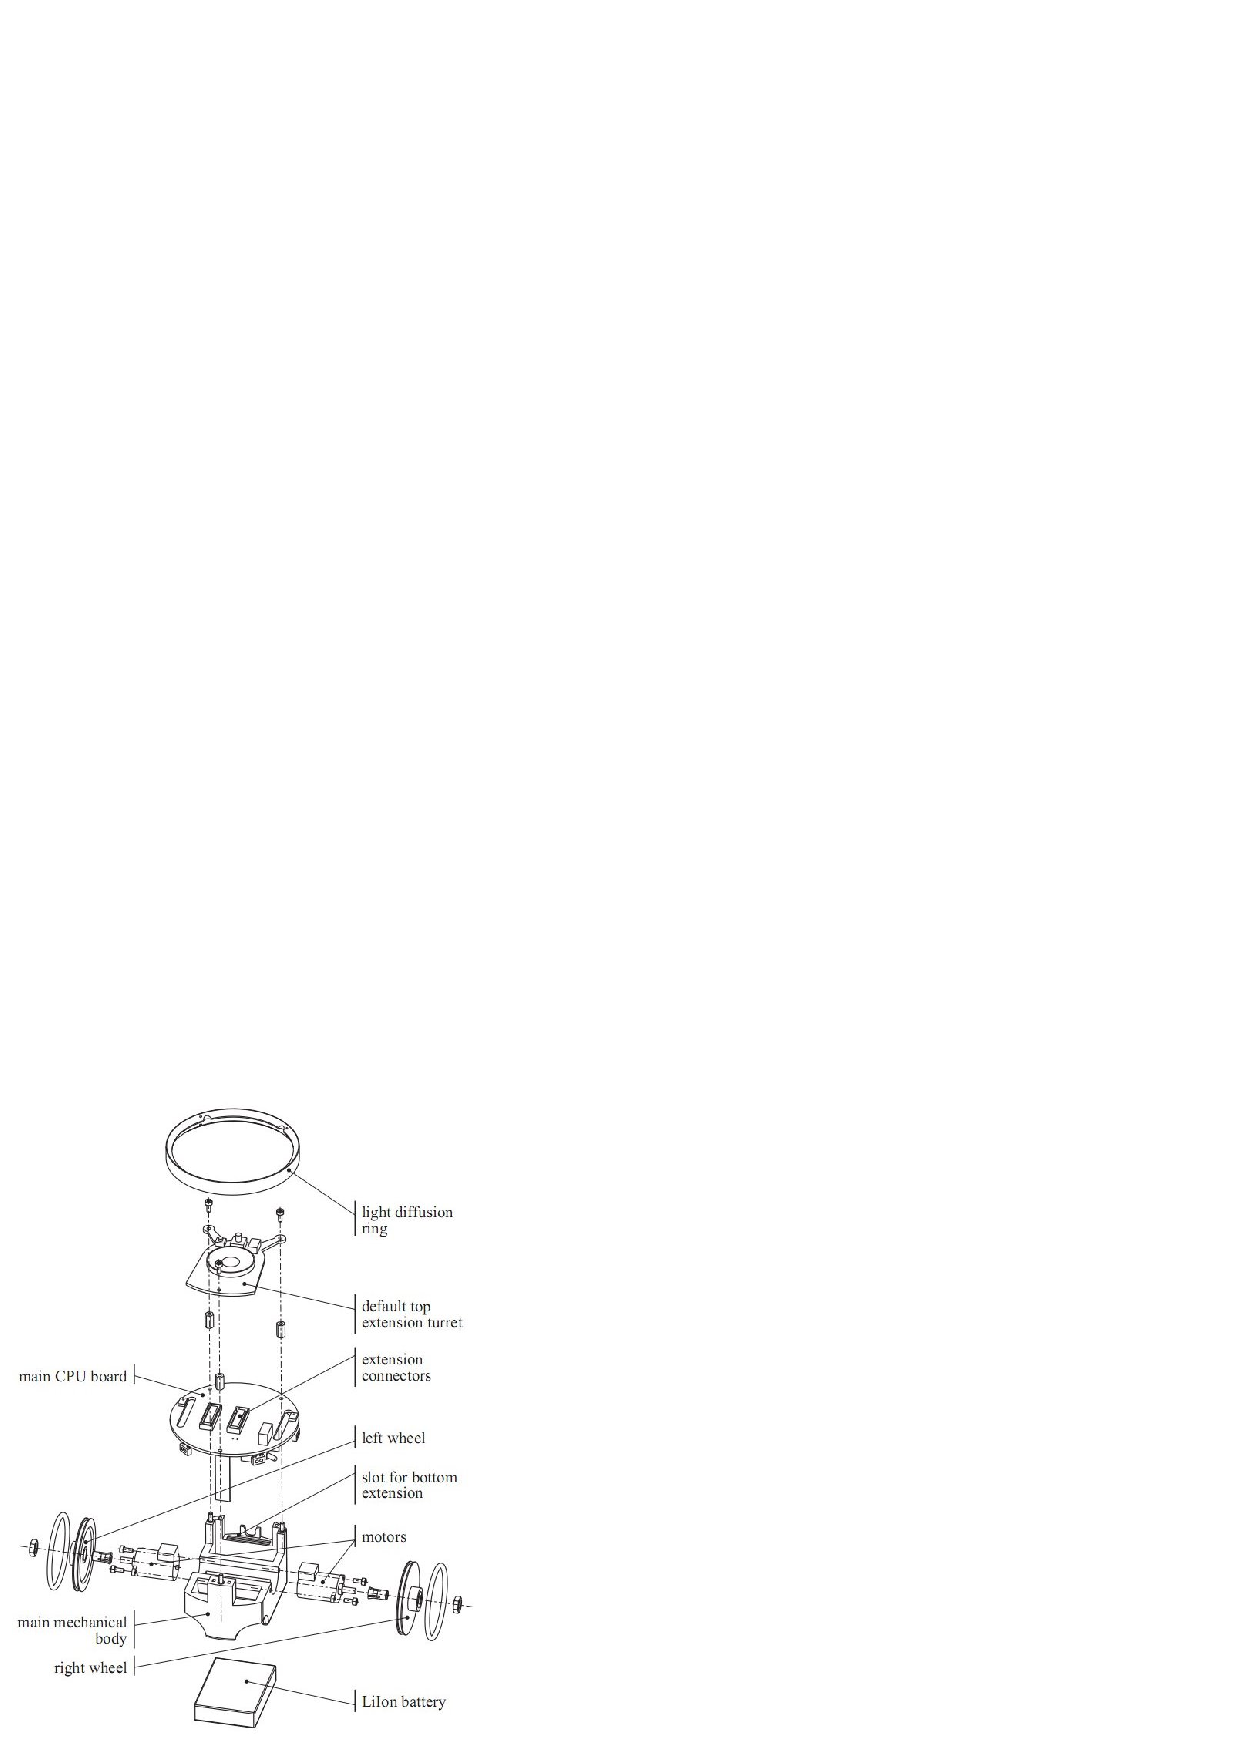
\includegraphics{epuck_str.pdf}}
    \end{picture}%
  \else
    \setlength{\unitlength}{1bp}%
    \begin{picture}(232.44, 320.96)(0,0)
    \put(0,0){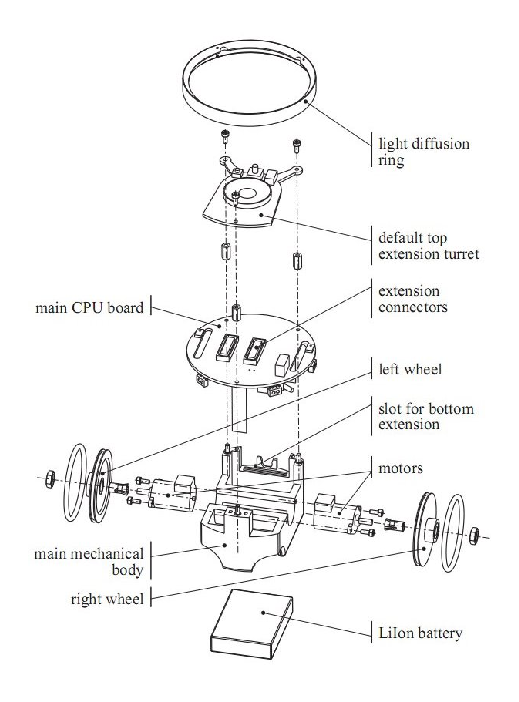
\includegraphics{epuck_str}}
    \end{picture}%
  \fi
  \caption{\label{pic:epuck_str}%
   Epuck structure \cite{robotica2009}}
  \end{figure}

  The mechanical design  is shown in Figure ~\ref{pic:epuck_str}.
  E-Puck consists of a rounded transparent body, a battery, two stepper motors with
  wheels on their axis, a printed circuit board, plastic ring of LEDs, 
  a camera and a default extension board.
  There are extensions like floor sensors, a rotating scanner or a turret with linear cameras,
  which can scale up e-Puck's sensors. If we are talking about e-Puck in this thesis,
  it is meant e-Puck only with the default extension.
  
  A default robot is more than 60 mm 
  high and it has a diameter of 75 mm. 
  The battery is placed in the bottom and can be easily extracted and recharged separately in a charger.
  Two stepper motors with wheels are screwed to a plastic body and are located on axis of e-Puck
  in order to allow robot turn around on place. Wheels has a diameter of 41 mm and the perch is 53 mm.
  Printed circuit board is fixed to the top of the body and there is ring of LEDs' around the board.
  A camera is placed on the front side of robot lying on the axis between the wheels.
  The extension board covers the main printed circuit board.
\section{Sensors, actuators and heart of a robot}
  Sensors and actuators determine the possibility of the robot usage.
  Luckily, e-Puck has a lot of sensors of different kinds and is equipped with typical actuators.
  The following paragraphs shortly describes e-Puck's sensors and actuators and mention a few problems 
  with transmitting data between the devices and PC using {\it BTCom}. {\it BTCom} protocol is used by {\it Elib},
  so {\it Elib} is to some extent dependent on {\it BTCom}.
  The actuators consist of motors, 8 red LEDs on perimeter, 4 green body LEDs,
   which are turned off and on together, a front LED and a speaker.
   
  Stepper motors are a great advantage of e-Puck, because the motion of wheel can be split
  into small steps. One wheel revolution corresponds to 1000 steps of motor. The 
  diameter of the wheel is 41 mm. If the wheel makes revolution, the wheel goes 128.8 mm. 
  In conclusion a thousand of steps matches 128.8 mm and one step is 0.128 mm. 
  Motors are equipped with encoders and the motors are very accurate, 
  which in combination with simple odometry really helps in localisation tasks.
  A nice feature of encoders is that their value can be set at any time.
  The maximum speed of the motors is one revolution per second in both directions.
  {\it BTCom} allows a programmer to set the speed of motors and also get and set the values
  of encoders.
   
  All e-Puck LEDs can be used for debugging or for making robot visible to other devices.
  Furthermore, the front LED can be used to illuminate the terrain in front of  e-Puck.
  Each LED can be turned off, turned on or set to an inverse state.
  
  Three axis accelerometers are placed inside the robots body. In the rest position
  the accelerometers measure the slant of e-Puck. They can also measure acceleration of e-Puck
  and for example detect a collision or a falling state of e-Puck. 
%	There is no problem with using accelerometer via {\it BTCom}.
  
  Infra Red (IR) sensors are typical sensors for mobile robotics. E-Puck has eight of them.
  Four are located in the front part of e-Puck, two are on both sides, two on back side.
  Sensors work in two modes. First they measure ambient infra red light.
  In the second mode IR sensors emit IR light and they measure reflected light, so 
  they can determine an obstacle, if it is near enough.
  Both functions are available in {\it BTCom}. 				
  Calibration of sensors increases the precision of detecting near obstacles.
  Infra red sensors are capable of recognising an obstacle under 4 cm.
  
  The Speaker together with microphones is a suitable communication tool between the people and e-Puck.
  On the other hand, a limited processing power of e-Puck does not allow to store and
   play complicated sounds. It is also impossible to use a speaker with microphones to speech
   recognition due to insufficient processing power.
  Despite the limitation of processing power the microphones can be easily used to locate
  the source of sound via amplitude measurement, because the microphones are placed near the perimeter
  in a triangle. Microphones measure current amplitude of sound. As exact distances between microphones 
  are known, we can compute frequency of the sound using Fast Fourier Transformation (FFT).
  Digital Signal Processor (DSP) is suitable for computing FFT,
   which will be introduced in this chapter.
  Maximal acquisition speed is 33 kHz. 
  For more information see \cite{sound}.
  
  A program which uses {\it BTCom} can capture values of amplitude only in irregular intervals, so 
  it is not possible to compute frequency of sound by running FFT on Personal Computer. 
  However to locate the source of sound is still possible.
  
  %\chapter{E-Puck}
\label{chap:epuck}
  An object of interest of a this thesis is a programming of the e-Puck robot and e-Puck itself.
  In this chapter e-Puck robot and its design is introduced. We focus on a programmer's point 
  of view of e-Puck qualities.
  For each sensor its functions, acceptable values and typical use is shortly presented. 
  After mentioning the e-Puck history the chapter continues with describing e-Puck's mechanical design and stepper motors. 
  The chapter finishes with a description of a e-Puck's camera and outlining e-Puck possibilities.
\section{Origin of e-Puck}
  E-Puck was developed in summer of 2004 at the �cole Polytechnique F�d�rale de Lausanne (EPFL) 
  as an open tool. E-Puck designers used open software and hardware development model. 
  Motivation for a new robot arose from an absence of a very small educational robot,
  which is sufficiently efficient, and can be used for education in many research areas.
  E-Puck can be applied in automatic control, signal processing or 
  distributed intelligent system research. E-Puck's structure is robust and simple to care about, 
  because e-Puck is intended to be used by students.
  Designers of e-Puck tried to use manufacturing components as much as possible 
  in order to keep the price low.		 
  
  The first generation of e-Pucks was replaced by the second stable generation from 2006.
  So far, more than 2000 robots have been manufactured.
  There are several distributors for Switzerland and America, one is in Japan
  \footnote{\url{http://www.roadnarrows.com/robotics/}, \url{http://www.aai.jp/}, \url{http://www.k-team.com/},
  \url{http://www.cyberbotics.com/products/robots/e-puck.html}, \url{http://www.gctronic.com/},
  \url{http://www.aai.ca/robots/e-puck.html}}.
  The price of e-Puck should be between 450 and 550 euro.%todo znak eura

\section{Mechanical Design}

  %\input{epuck_str.TpX} %pouzite \cite{robotica2009}
  \begin{figure}[!hbp]
  \centering
  \ifpdf
    \setlength{\unitlength}{1bp}%
    \begin{picture}(232.44, 320.96)(0,0)
    \put(0,0){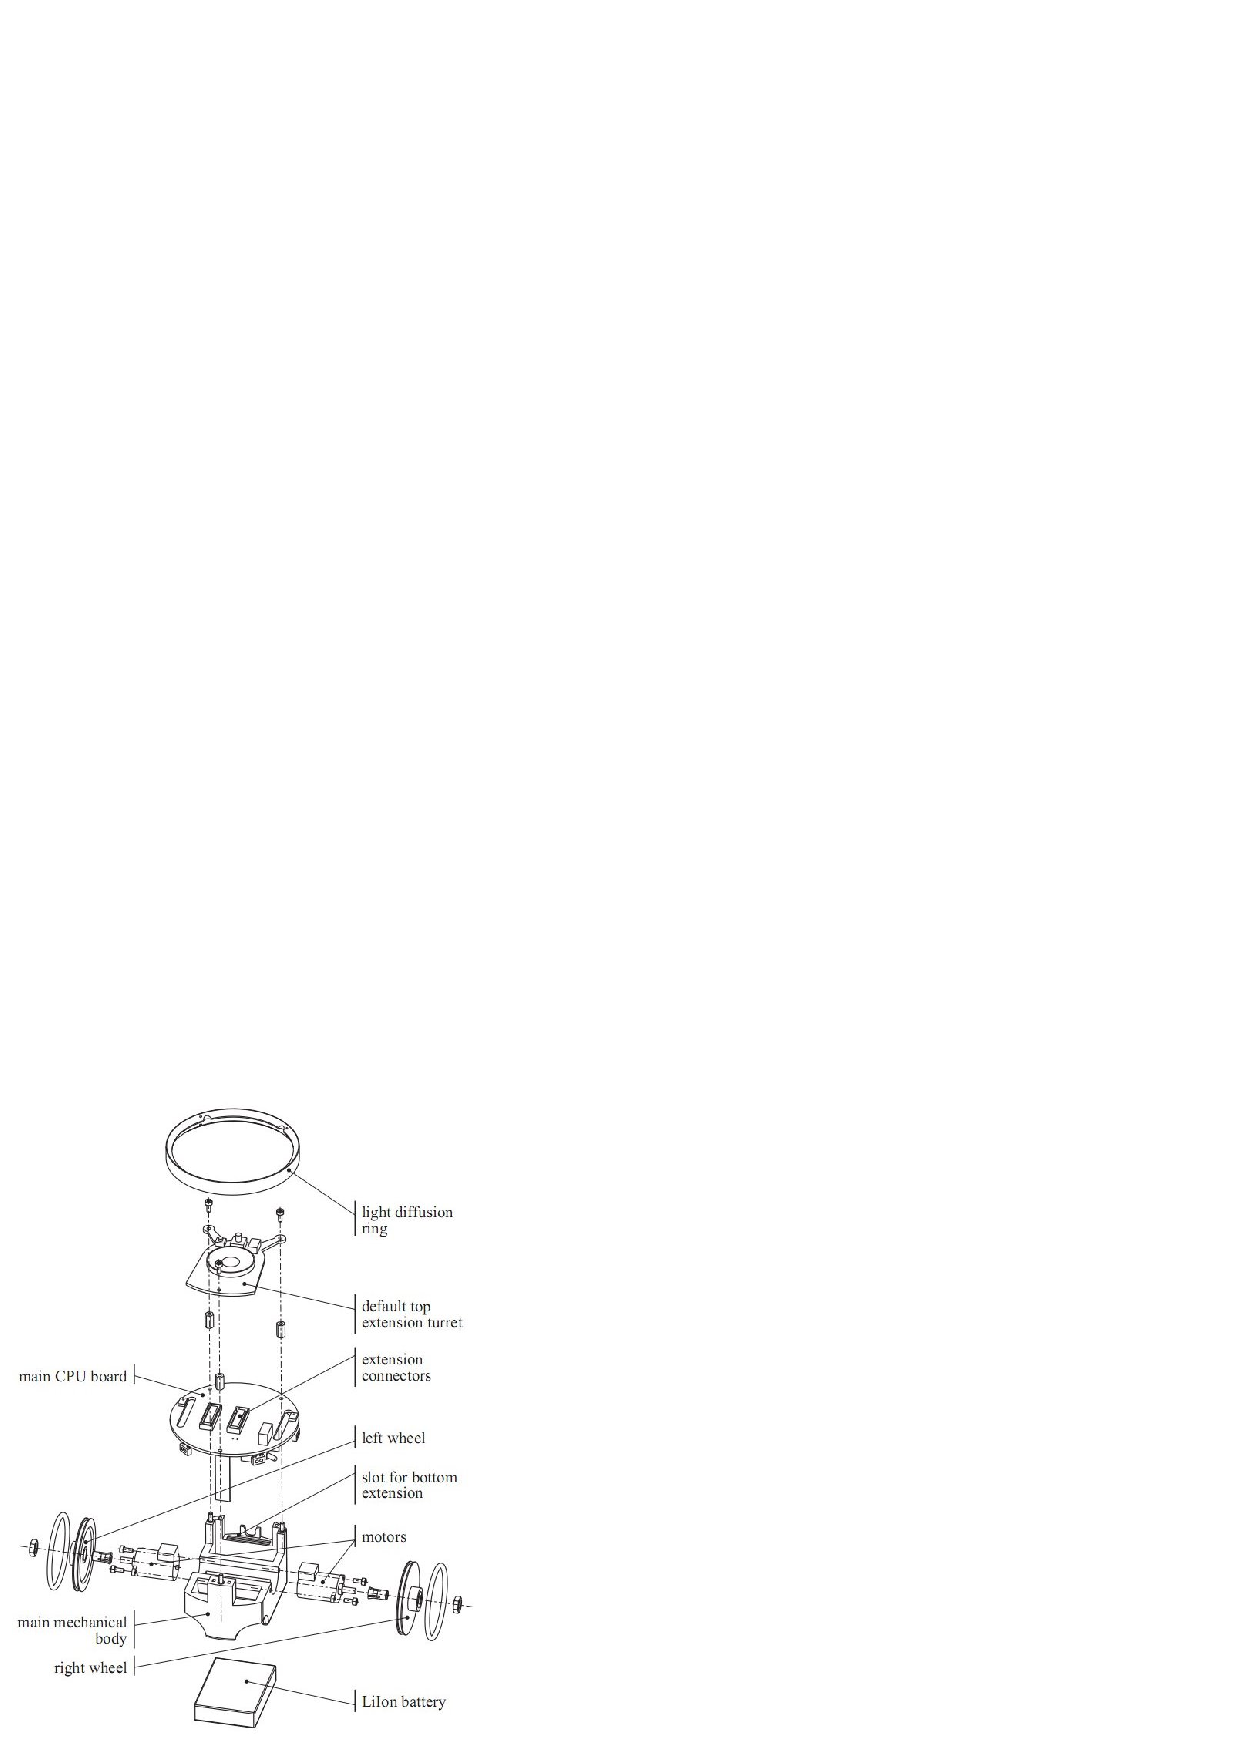
\includegraphics{epuck_str.pdf}}
    \end{picture}%
  \else
    \setlength{\unitlength}{1bp}%
    \begin{picture}(232.44, 320.96)(0,0)
    \put(0,0){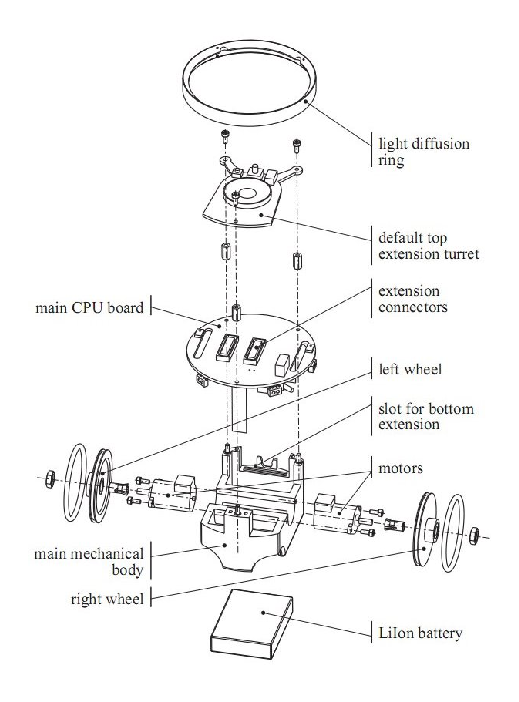
\includegraphics{epuck_str}}
    \end{picture}%
  \fi
  \caption{\label{pic:epuck_str}%
   Epuck structure \cite{robotica2009}}
  \end{figure}

  The mechanical design  is shown in Figure ~\ref{pic:epuck_str}.
  E-Puck consists of a rounded transparent body, a battery, two stepper motors with
  wheels on their axis, a printed circuit board, plastic ring of LEDs, 
  a camera and a default extension board.
  There are extensions like floor sensors, a rotating scanner or a turret with linear cameras,
  which can scale up e-Puck's sensors. If we are talking about e-Puck in this thesis,
  it is meant e-Puck only with the default extension.
  
  A default robot is more than 60 mm 
  high and it has a diameter of 75 mm. 
  The battery is placed in the bottom and can be easily extracted and recharged separately in a charger.
  Two stepper motors with wheels are screwed to a plastic body and are located on axis of e-Puck
  in order to allow robot turn around on place. Wheels has a diameter of 41 mm and the perch is 53 mm.
  Printed circuit board is fixed to the top of the body and there is ring of LEDs' around the board.
  A camera is placed on the front side of robot lying on the axis between the wheels.
  The extension board covers the main printed circuit board.
\section{Sensors, actuators and heart of a robot}
  Sensors and actuators determine the possibility of the robot usage.
  Luckily, e-Puck has a lot of sensors of different kinds and is equipped with typical actuators.
  The following paragraphs shortly describes e-Puck's sensors and actuators and mention a few problems 
  with transmitting data between the devices and PC using {\it BTCom}. {\it BTCom} protocol is used by {\it Elib},
  so {\it Elib} is to some extent dependent on {\it BTCom}.
  The actuators consist of motors, 8 red LEDs on perimeter, 4 green body LEDs,
   which are turned off and on together, a front LED and a speaker.
   
  Stepper motors are a great advantage of e-Puck, because the motion of wheel can be split
  into small steps. One wheel revolution corresponds to 1000 steps of motor. The 
  diameter of the wheel is 41 mm. If the wheel makes revolution, the wheel goes 128.8 mm. 
  In conclusion a thousand of steps matches 128.8 mm and one step is 0.128 mm. 
  Motors are equipped with encoders and the motors are very accurate, 
  which in combination with simple odometry really helps in localisation tasks.
  A nice feature of encoders is that their value can be set at any time.
  The maximum speed of the motors is one revolution per second in both directions.
  {\it BTCom} allows a programmer to set the speed of motors and also get and set the values
  of encoders.
   
  All e-Puck LEDs can be used for debugging or for making robot visible to other devices.
  Furthermore, the front LED can be used to illuminate the terrain in front of  e-Puck.
  Each LED can be turned off, turned on or set to an inverse state.
  
  Three axis accelerometers are placed inside the robots body. In the rest position
  the accelerometers measure the slant of e-Puck. They can also measure acceleration of e-Puck
  and for example detect a collision or a falling state of e-Puck. 
%	There is no problem with using accelerometer via {\it BTCom}.
  
  Infra Red (IR) sensors are typical sensors for mobile robotics. E-Puck has eight of them.
  Four are located in the front part of e-Puck, two are on both sides, two on back side.
  Sensors work in two modes. First they measure ambient infra red light.
  In the second mode IR sensors emit IR light and they measure reflected light, so 
  they can determine an obstacle, if it is near enough.
  Both functions are available in {\it BTCom}. 				
  Calibration of sensors increases the precision of detecting near obstacles.
  Infra red sensors are capable of recognising an obstacle under 4 cm.
  
  The Speaker together with microphones is a suitable communication tool between the people and e-Puck.
  On the other hand, a limited processing power of e-Puck does not allow to store and
   play complicated sounds. It is also impossible to use a speaker with microphones to speech
   recognition due to insufficient processing power.
  Despite the limitation of processing power the microphones can be easily used to locate
  the source of sound via amplitude measurement, because the microphones are placed near the perimeter
  in a triangle. Microphones measure current amplitude of sound. As exact distances between microphones 
  are known, we can compute frequency of the sound using Fast Fourier Transformation (FFT).
  Digital Signal Processor (DSP) is suitable for computing FFT,
   which will be introduced in this chapter.
  Maximal acquisition speed is 33 kHz. 
  For more information see \cite{sound}.
  
  A program which uses {\it BTCom} can capture values of amplitude only in irregular intervals, so 
  it is not possible to compute frequency of sound by running FFT on Personal Computer. 
  However to locate the source of sound is still possible.
  
  %\chapter{E-Puck}
\label{chap:epuck}
  An object of interest of a this thesis is a programming of the e-Puck robot and e-Puck itself.
  In this chapter e-Puck robot and its design is introduced. We focus on a programmer's point 
  of view of e-Puck qualities.
  For each sensor its functions, acceptable values and typical use is shortly presented. 
  After mentioning the e-Puck history the chapter continues with describing e-Puck's mechanical design and stepper motors. 
  The chapter finishes with a description of a e-Puck's camera and outlining e-Puck possibilities.
\section{Origin of e-Puck}
  E-Puck was developed in summer of 2004 at the �cole Polytechnique F�d�rale de Lausanne (EPFL) 
  as an open tool. E-Puck designers used open software and hardware development model. 
  Motivation for a new robot arose from an absence of a very small educational robot,
  which is sufficiently efficient, and can be used for education in many research areas.
  E-Puck can be applied in automatic control, signal processing or 
  distributed intelligent system research. E-Puck's structure is robust and simple to care about, 
  because e-Puck is intended to be used by students.
  Designers of e-Puck tried to use manufacturing components as much as possible 
  in order to keep the price low.		 
  
  The first generation of e-Pucks was replaced by the second stable generation from 2006.
  So far, more than 2000 robots have been manufactured.
  There are several distributors for Switzerland and America, one is in Japan
  \footnote{\url{http://www.roadnarrows.com/robotics/}, \url{http://www.aai.jp/}, \url{http://www.k-team.com/},
  \url{http://www.cyberbotics.com/products/robots/e-puck.html}, \url{http://www.gctronic.com/},
  \url{http://www.aai.ca/robots/e-puck.html}}.
  The price of e-Puck should be between 450 and 550 euro.%todo znak eura

\section{Mechanical Design}

  %\input{epuck_str.TpX} %pouzite \cite{robotica2009}
  \begin{figure}[!hbp]
  \centering
  \ifpdf
    \setlength{\unitlength}{1bp}%
    \begin{picture}(232.44, 320.96)(0,0)
    \put(0,0){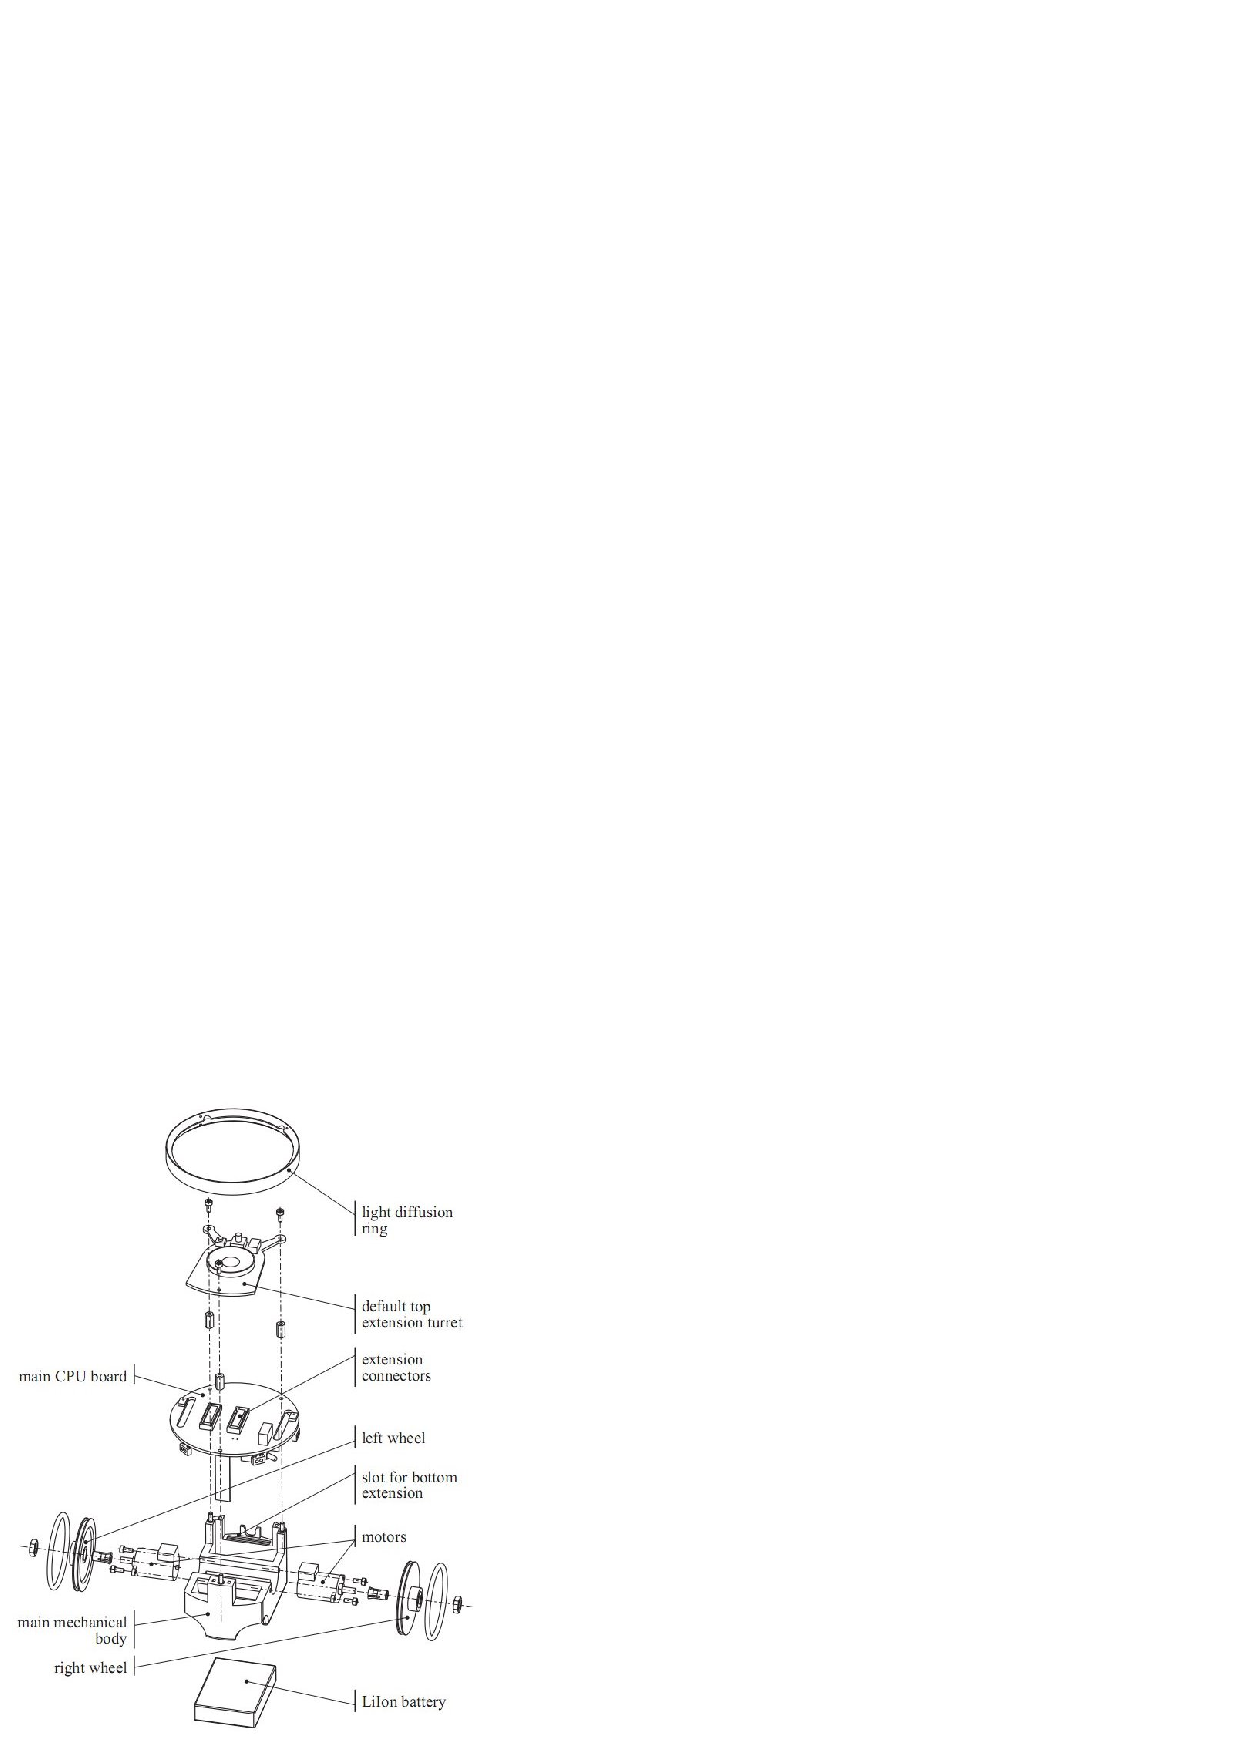
\includegraphics{epuck_str.pdf}}
    \end{picture}%
  \else
    \setlength{\unitlength}{1bp}%
    \begin{picture}(232.44, 320.96)(0,0)
    \put(0,0){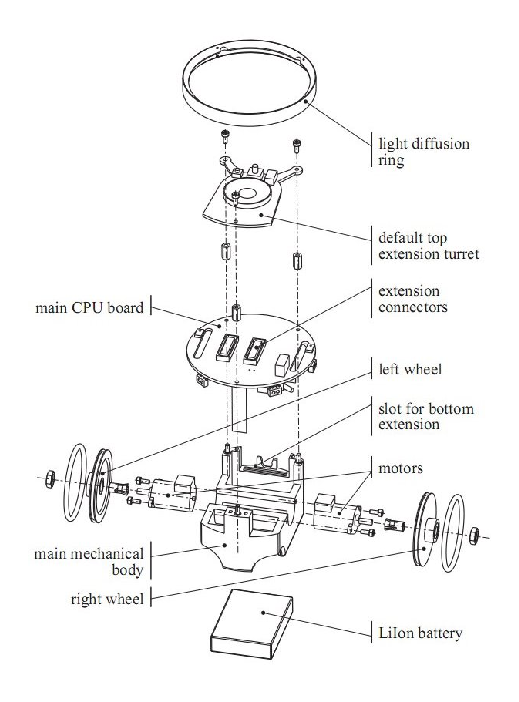
\includegraphics{epuck_str}}
    \end{picture}%
  \fi
  \caption{\label{pic:epuck_str}%
   Epuck structure \cite{robotica2009}}
  \end{figure}

  The mechanical design  is shown in Figure ~\ref{pic:epuck_str}.
  E-Puck consists of a rounded transparent body, a battery, two stepper motors with
  wheels on their axis, a printed circuit board, plastic ring of LEDs, 
  a camera and a default extension board.
  There are extensions like floor sensors, a rotating scanner or a turret with linear cameras,
  which can scale up e-Puck's sensors. If we are talking about e-Puck in this thesis,
  it is meant e-Puck only with the default extension.
  
  A default robot is more than 60 mm 
  high and it has a diameter of 75 mm. 
  The battery is placed in the bottom and can be easily extracted and recharged separately in a charger.
  Two stepper motors with wheels are screwed to a plastic body and are located on axis of e-Puck
  in order to allow robot turn around on place. Wheels has a diameter of 41 mm and the perch is 53 mm.
  Printed circuit board is fixed to the top of the body and there is ring of LEDs' around the board.
  A camera is placed on the front side of robot lying on the axis between the wheels.
  The extension board covers the main printed circuit board.
\section{Sensors, actuators and heart of a robot}
  Sensors and actuators determine the possibility of the robot usage.
  Luckily, e-Puck has a lot of sensors of different kinds and is equipped with typical actuators.
  The following paragraphs shortly describes e-Puck's sensors and actuators and mention a few problems 
  with transmitting data between the devices and PC using {\it BTCom}. {\it BTCom} protocol is used by {\it Elib},
  so {\it Elib} is to some extent dependent on {\it BTCom}.
  The actuators consist of motors, 8 red LEDs on perimeter, 4 green body LEDs,
   which are turned off and on together, a front LED and a speaker.
   
  Stepper motors are a great advantage of e-Puck, because the motion of wheel can be split
  into small steps. One wheel revolution corresponds to 1000 steps of motor. The 
  diameter of the wheel is 41 mm. If the wheel makes revolution, the wheel goes 128.8 mm. 
  In conclusion a thousand of steps matches 128.8 mm and one step is 0.128 mm. 
  Motors are equipped with encoders and the motors are very accurate, 
  which in combination with simple odometry really helps in localisation tasks.
  A nice feature of encoders is that their value can be set at any time.
  The maximum speed of the motors is one revolution per second in both directions.
  {\it BTCom} allows a programmer to set the speed of motors and also get and set the values
  of encoders.
   
  All e-Puck LEDs can be used for debugging or for making robot visible to other devices.
  Furthermore, the front LED can be used to illuminate the terrain in front of  e-Puck.
  Each LED can be turned off, turned on or set to an inverse state.
  
  Three axis accelerometers are placed inside the robots body. In the rest position
  the accelerometers measure the slant of e-Puck. They can also measure acceleration of e-Puck
  and for example detect a collision or a falling state of e-Puck. 
%	There is no problem with using accelerometer via {\it BTCom}.
  
  Infra Red (IR) sensors are typical sensors for mobile robotics. E-Puck has eight of them.
  Four are located in the front part of e-Puck, two are on both sides, two on back side.
  Sensors work in two modes. First they measure ambient infra red light.
  In the second mode IR sensors emit IR light and they measure reflected light, so 
  they can determine an obstacle, if it is near enough.
  Both functions are available in {\it BTCom}. 				
  Calibration of sensors increases the precision of detecting near obstacles.
  Infra red sensors are capable of recognising an obstacle under 4 cm.
  
  The Speaker together with microphones is a suitable communication tool between the people and e-Puck.
  On the other hand, a limited processing power of e-Puck does not allow to store and
   play complicated sounds. It is also impossible to use a speaker with microphones to speech
   recognition due to insufficient processing power.
  Despite the limitation of processing power the microphones can be easily used to locate
  the source of sound via amplitude measurement, because the microphones are placed near the perimeter
  in a triangle. Microphones measure current amplitude of sound. As exact distances between microphones 
  are known, we can compute frequency of the sound using Fast Fourier Transformation (FFT).
  Digital Signal Processor (DSP) is suitable for computing FFT,
   which will be introduced in this chapter.
  Maximal acquisition speed is 33 kHz. 
  For more information see \cite{sound}.
  
  A program which uses {\it BTCom} can capture values of amplitude only in irregular intervals, so 
  it is not possible to compute frequency of sound by running FFT on Personal Computer. 
  However to locate the source of sound is still possible.
  
  %\input{epuck.TpX}
  \begin{figure}[!hbp]
  \centering
  \ifpdf
    \setlength{\unitlength}{1bp}%
    \begin{picture}(228.66, 174.33)(0,0)
    \put(0,0){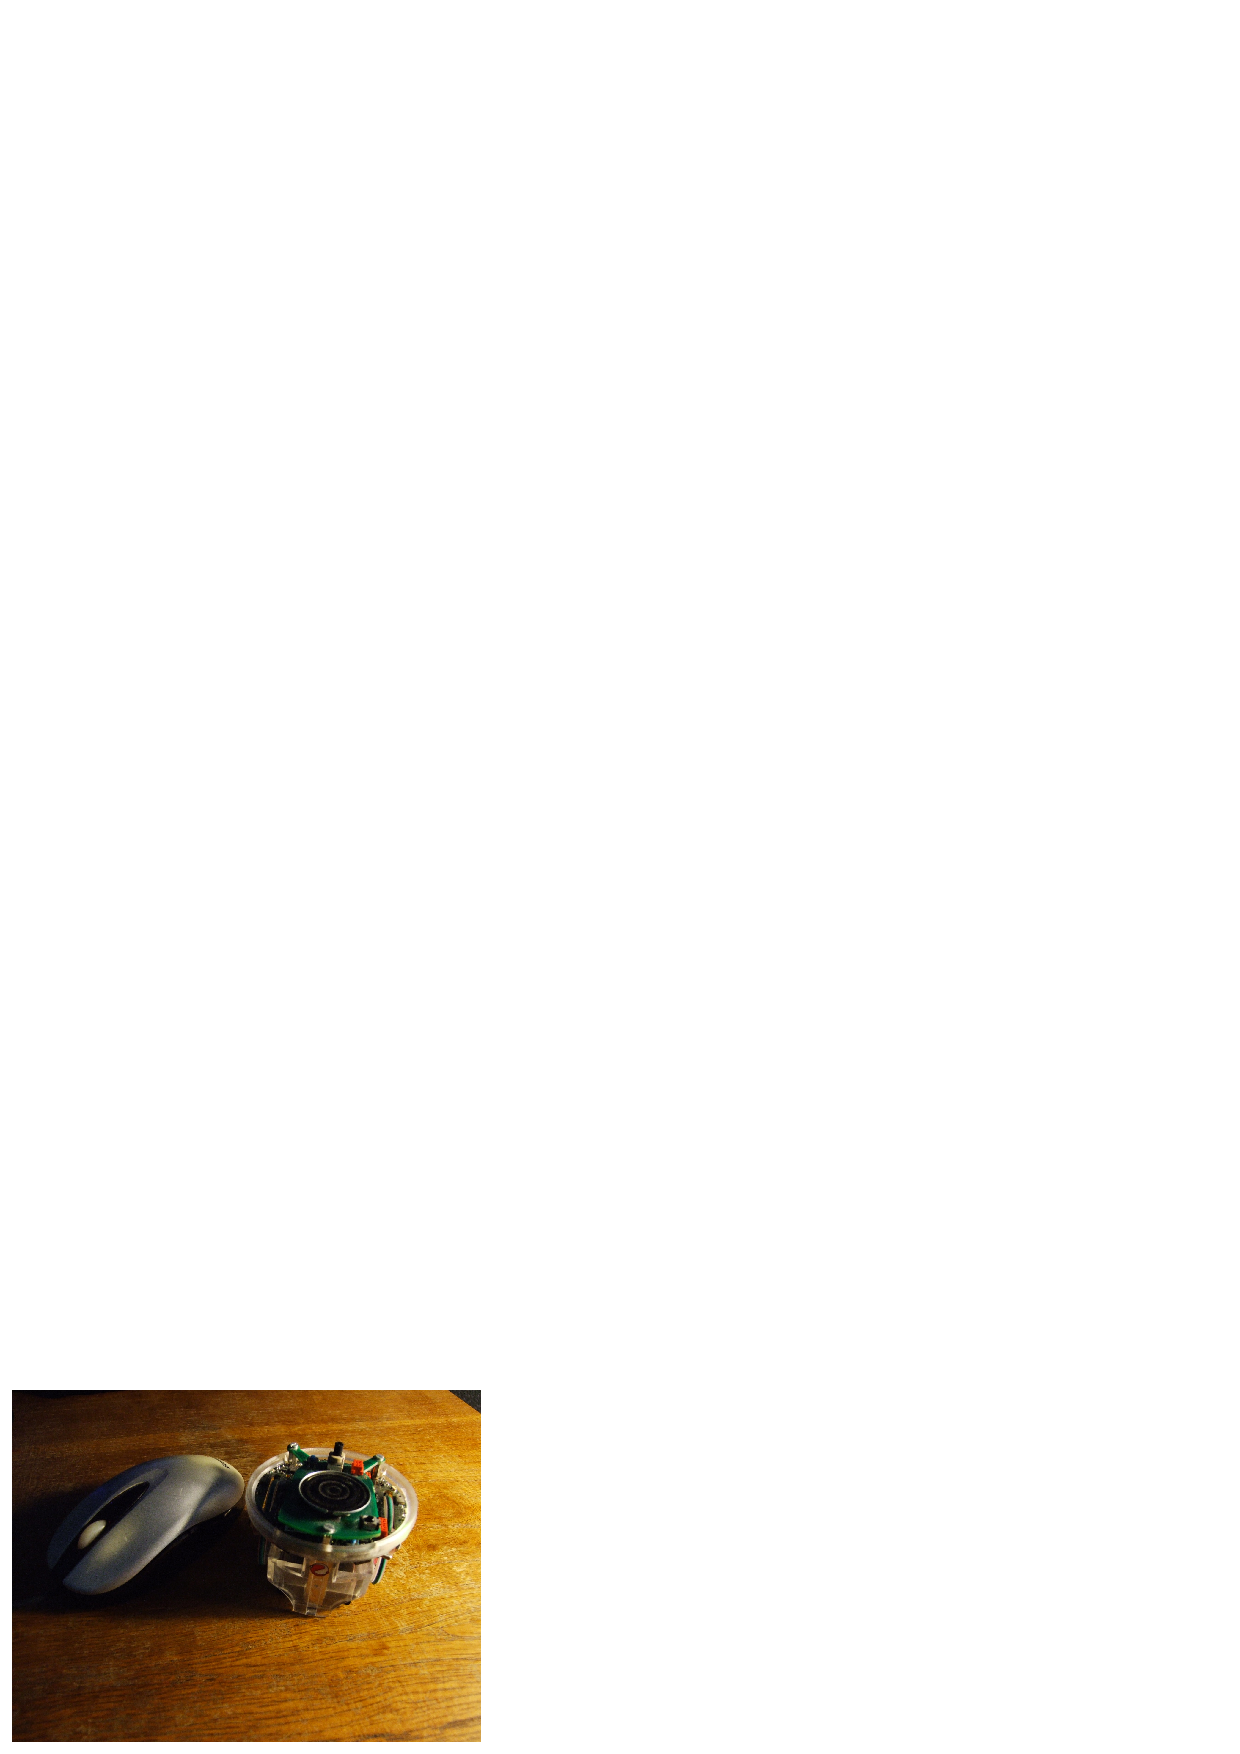
\includegraphics{epuck.pdf}}
    \end{picture}%
  \else
    \setlength{\unitlength}{1bp}%
    \begin{picture}(228.66, 174.33)(0,0)
    \put(0,0){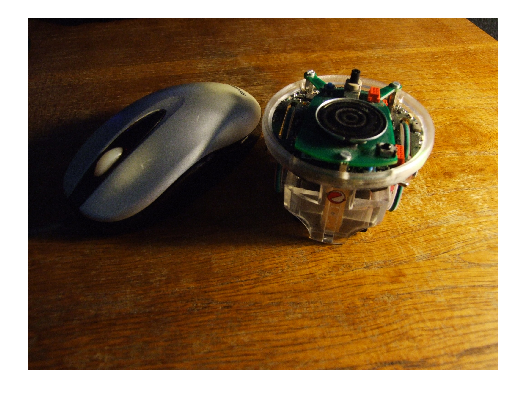
\includegraphics{epuck}}
    \end{picture}%
  \fi
  \caption{\label{pic:epuck}%
   E-Puck avoiding a mouse}
  \end{figure}

  %todo what is zoom? does it only narrow field of view? or does it make the picture look closer?
  E-Puck's camera is a colour CMOS camera with 640 * 480 resolution. 
  Because only 8 kB of RAM memory is available and a part of it is used by running program,
  the picture size has to be reduced in order to save the image in a memory.
  The image processing is really demanding on the processing power so it is not 
  convenient to be run on the slow e-Puck's processor.
  
  On the other hand, using {\it BTCom} solves the problem with limited processing power
  by sending picture to Personal Computer (PC). PC has enough resources to process the image fast,
   but the transport of an image takes a long time too. 
   For example capturing and sending a colour image of size 40 * 40 pixels 
  takes more than 0.2 seconds, if it is sent over Bluetooth.
  {\it BTCom} can set height, width, colour mode and zoom. A colourful picture is twice as big as the same picture taken
  in grey scale mode.
   Zoom has three acceptable values 1, 4 and 8. One is for the biggest zoom, 8 represents the smallest.
  Width and height are limited only by the size of the available memory in e-Puck.
  
  Processor, dsPIC 30F6014, is the heart of e-Puck and runs at 60 MHz, which correspond to 15 MIPS.
  It has C oriented instructions and supports compiling from GNU compilers.
  Apart from standard 16 bits core unit Digital Signal Processor brings very high performance for computation,
  for example FFT or other signal processing.
  Programs can be downloaded to flash memory with 144 kB and
   are loaded to RAM memory according to the selector position.
  E-Puck's RAM memory has only 8 kB. A currently running program and all its data are placed in RAM memory.
  
  Communication with other devices is provided by Bluetooth and RS232 serial interface.
  Both, Bluetooth and RS232, can be used to download programs to e-Puck's flash memory.
  In addition, Bluetooth can be used to communicate with other e-Pucks or with a computer
  using {\it BTCom}. 
  The counter part of {\it BTCom} on computer is connected to the serial port.


  \begin{figure}[!hbp]
  \centering
  \ifpdf
    \setlength{\unitlength}{1bp}%
    \begin{picture}(228.66, 174.33)(0,0)
    \put(0,0){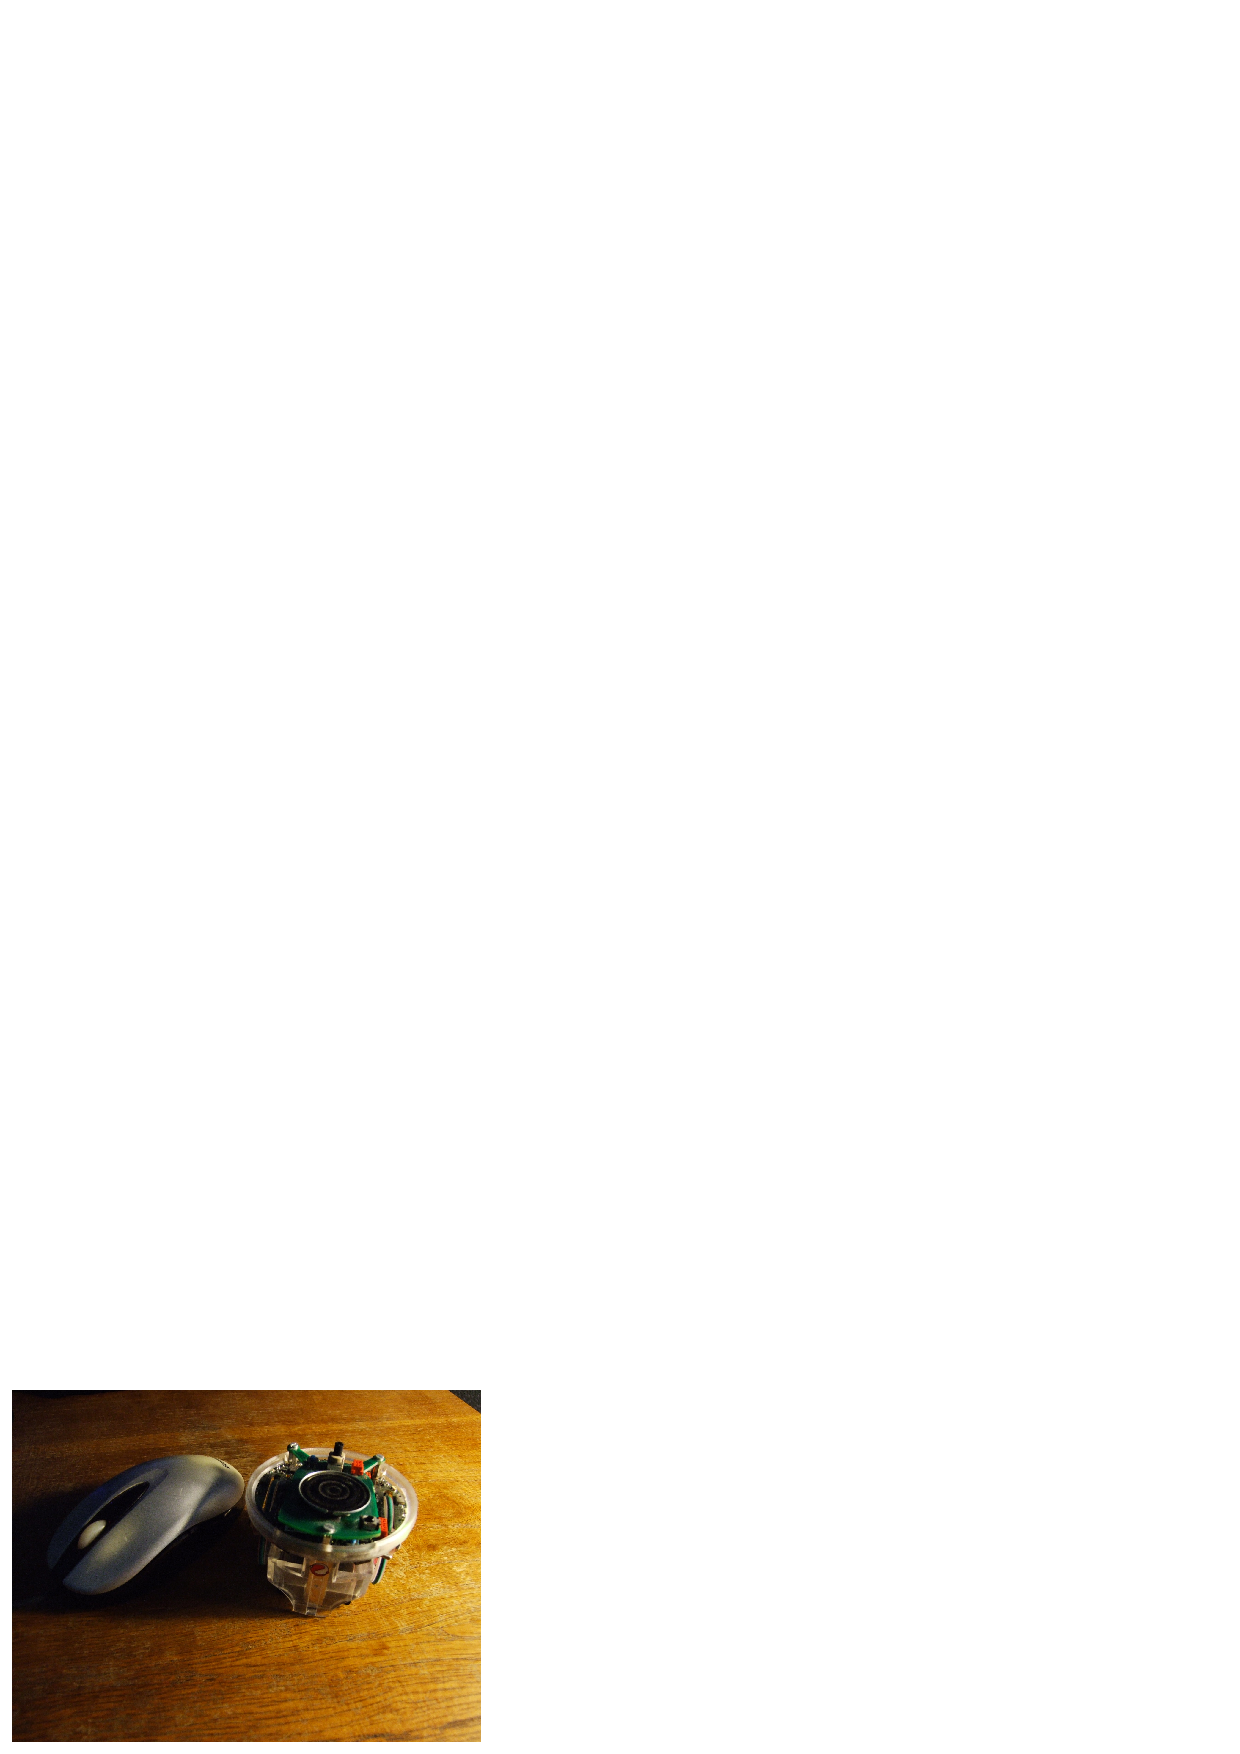
\includegraphics{epuck.pdf}}
    \end{picture}%
  \else
    \setlength{\unitlength}{1bp}%
    \begin{picture}(228.66, 174.33)(0,0)
    \put(0,0){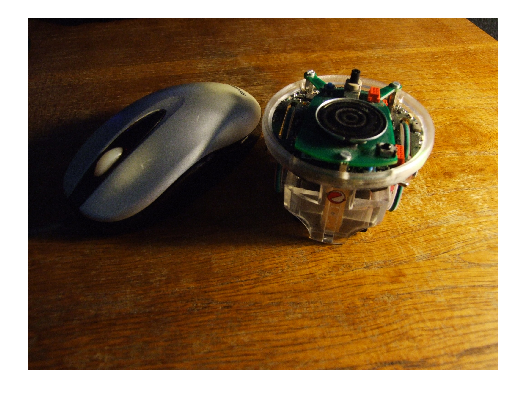
\includegraphics{epuck}}
    \end{picture}%
  \fi
  \caption{\label{pic:epuck}%
   E-Puck avoiding a mouse}
  \end{figure}

  %todo what is zoom? does it only narrow field of view? or does it make the picture look closer?
  E-Puck's camera is a colour CMOS camera with 640 * 480 resolution. 
  Because only 8 kB of RAM memory is available and a part of it is used by running program,
  the picture size has to be reduced in order to save the image in a memory.
  The image processing is really demanding on the processing power so it is not 
  convenient to be run on the slow e-Puck's processor.
  
  On the other hand, using {\it BTCom} solves the problem with limited processing power
  by sending picture to Personal Computer (PC). PC has enough resources to process the image fast,
   but the transport of an image takes a long time too. 
   For example capturing and sending a colour image of size 40 * 40 pixels 
  takes more than 0.2 seconds, if it is sent over Bluetooth.
  {\it BTCom} can set height, width, colour mode and zoom. A colourful picture is twice as big as the same picture taken
  in grey scale mode.
   Zoom has three acceptable values 1, 4 and 8. One is for the biggest zoom, 8 represents the smallest.
  Width and height are limited only by the size of the available memory in e-Puck.
  
  Processor, dsPIC 30F6014, is the heart of e-Puck and runs at 60 MHz, which correspond to 15 MIPS.
  It has C oriented instructions and supports compiling from GNU compilers.
  Apart from standard 16 bits core unit Digital Signal Processor brings very high performance for computation,
  for example FFT or other signal processing.
  Programs can be downloaded to flash memory with 144 kB and
   are loaded to RAM memory according to the selector position.
  E-Puck's RAM memory has only 8 kB. A currently running program and all its data are placed in RAM memory.
  
  Communication with other devices is provided by Bluetooth and RS232 serial interface.
  Both, Bluetooth and RS232, can be used to download programs to e-Puck's flash memory.
  In addition, Bluetooth can be used to communicate with other e-Pucks or with a computer
  using {\it BTCom}. 
  The counter part of {\it BTCom} on computer is connected to the serial port.


  \begin{figure}[!hbp]
  \centering
  \ifpdf
    \setlength{\unitlength}{1bp}%
    \begin{picture}(228.66, 174.33)(0,0)
    \put(0,0){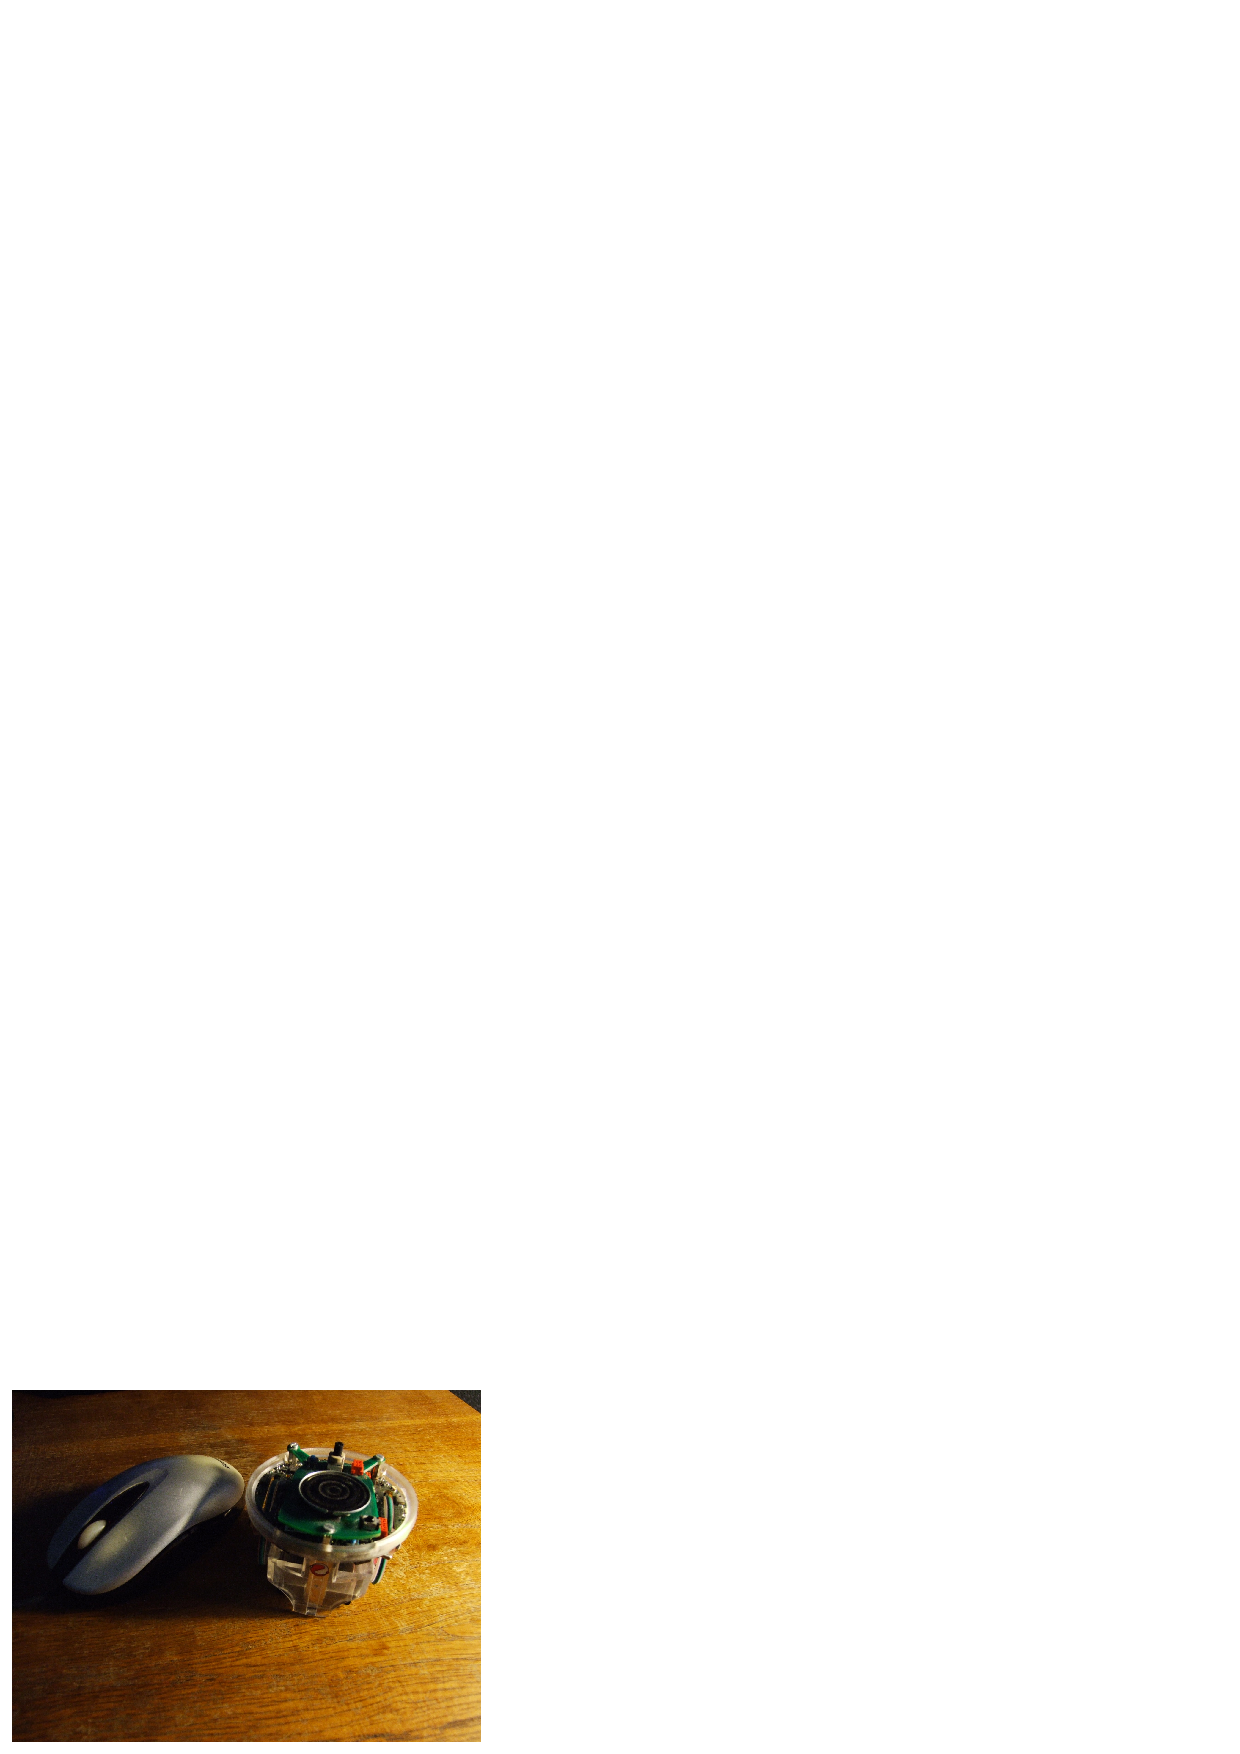
\includegraphics{epuck.pdf}}
    \end{picture}%
  \else
    \setlength{\unitlength}{1bp}%
    \begin{picture}(228.66, 174.33)(0,0)
    \put(0,0){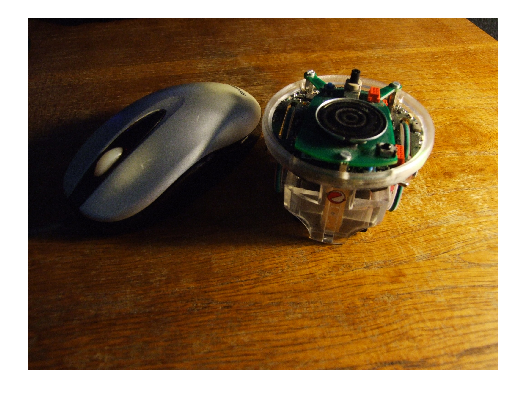
\includegraphics{epuck}}
    \end{picture}%
  \fi
  \caption{\label{pic:epuck}%
   E-Puck avoiding a mouse}
  \end{figure}

  %todo what is zoom? does it only narrow field of view? or does it make the picture look closer?
  E-Puck's camera is a colour CMOS camera with 640 * 480 resolution. 
  Because only 8 kB of RAM memory is available and a part of it is used by running program,
  the picture size has to be reduced in order to save the image in a memory.
  The image processing is really demanding on the processing power so it is not 
  convenient to be run on the slow e-Puck's processor.
  
  On the other hand, using {\it BTCom} solves the problem with limited processing power
  by sending picture to Personal Computer (PC). PC has enough resources to process the image fast,
   but the transport of an image takes a long time too. 
   For example capturing and sending a colour image of size 40 * 40 pixels 
  takes more than 0.2 seconds, if it is sent over Bluetooth.
  {\it BTCom} can set height, width, colour mode and zoom. A colourful picture is twice as big as the same picture taken
  in grey scale mode.
   Zoom has three acceptable values 1, 4 and 8. One is for the biggest zoom, 8 represents the smallest.
  Width and height are limited only by the size of the available memory in e-Puck.
  
  Processor, dsPIC 30F6014, is the heart of e-Puck and runs at 60 MHz, which correspond to 15 MIPS.
  It has C oriented instructions and supports compiling from GNU compilers.
  Apart from standard 16 bits core unit Digital Signal Processor brings very high performance for computation,
  for example FFT or other signal processing.
  Programs can be downloaded to flash memory with 144 kB and
   are loaded to RAM memory according to the selector position.
  E-Puck's RAM memory has only 8 kB. A currently running program and all its data are placed in RAM memory.
  
  Communication with other devices is provided by Bluetooth and RS232 serial interface.
  Both, Bluetooth and RS232, can be used to download programs to e-Puck's flash memory.
  In addition, Bluetooth can be used to communicate with other e-Pucks or with a computer
  using {\it BTCom}. 
  The counter part of {\it BTCom} on computer is connected to the serial port.


	%todo what is zoom? does it only narrow field of view? or does it make the picture look closer?
	E-Puck's camera is a colour CMOS camera with 640 * 480 resolution. 
	Because only 8 kB of RAM memory is available and a part of it is used by running program,
	the picture size has to be reduced in order to save the image in a memory.
	The image processing is really demanding on the processing power so it is not 
	convenient to be run on the slow e-Puck's processor.
	
	On the other hand, using {\it BTCom} solves the problem with limited processing power
	by sending picture to Personal Computer (PC). PC has enough resources to process the image fast,
	 but the transport of an image takes a long time too. 
	 For example capturing and sending a colour image of size 40 * 40 pixels 
	takes more than 0.2 seconds, if it is sent over Bluetooth.
	{\it BTCom} can set height, width, colour mode and zoom. A colourful picture is twice as big as the same picture taken
	in grey scale mode.
	 Zoom has three acceptable values 1, 4 and 8. One is for the biggest zoom, 8 represents the smallest.
	Width and height are limited only by the size of the available memory in e-Puck.
	
	Processor, dsPIC 30F6014, is the heart of e-Puck and runs at 60 MHz, which correspond to 15 MIPS.
	It has C oriented instructions and supports compiling from GNU compilers.
	Apart from standard 16 bits core unit Digital Signal Processor brings very high performance for computation,
	for example FFT or other signal processing.
	Programs can be downloaded to flash memory with 144 kB and
	 are loaded to RAM memory according to the selector position.
	E-Puck's RAM memory has only 8 kB. A currently running program and all its data are placed in RAM memory.
	
	Communication with other devices is provided by Bluetooth and RS232 serial interface.
	Both, Bluetooth and RS232, can be used to download programs to e-Puck's flash memory.
	In addition, Bluetooth can be used to communicate with other e-Pucks or with a computer
	using {\it BTCom}. 
	The counter part of {\it BTCom} on computer is connected to the serial port.

%%%%%%%%%%%%%%%%%%%%%%%%%%%%%%%%%%%%%%%%%%%%%%%%%%%%%%%%%%%%%%%%%%%%%%%%%%%%%%%%%%%%%%%%%%%%%%%%%%%%%%%%%%
\chapter{Available software} \label{chap:software}
	In this chapter we shortly introduce software which helps programmer
	to debug and develop a program for a robot control. Only simulators will be introduced, because 
	there is no available program or library for e-Puck like {\it Elib},
	which controls e-Puck remotely and asynchronously from PC.
	All introduced simulators run at PC and allow user to control and program a virtual copy of robot.
	Most of the simulators simplify physics and construction, although they try to simulate sensors
	and actuators as faithfully as possible. Some of the simulators support porting the program,
	which has been created for the virtual robot, to real robot.
	
\section{Why simulators, why remote control?}
	{\it Elib} and the simulators benefit from moving the debugging environment from the robot to PC.
	PC has enough resources at disposal and the code can be debugged much more comfortably. Debugging
	tools depend on the structure of simulator and a programming language which is used by the simulator.
	{\it Elib} and the simulators allow to stop the program at any time.
	
	{\it Elib} uses $C\#$, which can be developed in Microsoft Visual Studio or MonoDevelop Studio.
	Both studios support many features like setting breakpoints with conditions, call stack table,
	manual switching between threads and so on.
	
	The simulators have several advantages over robot remote control.
	A simulator provides the developer with a consistent behaviour of a virtual robot.
	A programmer has for example battery level under control. 
	The virtual robot measures in same situations identical values from its sensors. 
	
	The real robot is strongly influenced by the state of the battery
	and measures a completely different values in the same situation.
	Great advantage of the simulators is the possibility of not only stopping
	the running program, but also freezing the simulated environment. 
	
	Simulators also do not need a real robot for testing a program, which is extremely
	useful in the class with many students where only a few robots are available.
	Some of the simulators are completely free, which is certainly a nice quality.
	
	On the other hand, a remote control of a robot has some benefits too. 
	A lot of unpredictable situations are not simulated in simulators, although 
	many simulators have the option to involve randomness. The robot usually
	needs to be tested in the real environment too.
	
	Let us note, that simulators use physical and graphical engines. They are demanding applications
	for PC. 
	%todo rozvest co je fyzikalni engine? kde je to pouzivany v hrach, v simulatorech obejit napriklad citaci
	On the other hand, remote control is simple fast application.
	
	Last but not least, playing with real robot is simply much more entertaining. 	
	It motivates the users to solve real problems including hardware set up. 
	During programming a real robot the typical problems of mobile robotics are touch on.
	Simulators do not motivate the users to cope with a changing environment or an inaccurate odometry.
	
	In following subsections the simulators listed below will be discussed:
	\begin{itemize}
	\item Microsoft Robotics Developer Studio\cite{msrs} is a complex tool based on message sending.
	\item Player/Stage\cite{player} (Gazebo) is an open source project developed in C++, which is widely used.
	\item Pyrobot(Pyro)\cite{pyro} is also an open source project written in Python. It supports abstract
	interfaces for devices convenient for e-Puck.
	\item Enki\cite{enki} is a fast simulation tool for a big population of robots.
	\item Commercial simulator Webots\cite{webots} is the only simulator, which almost fully support e-Puck. 
	\end{itemize}
\section{Microsoft Robotics Developer Studio\cite{msrs}} 
	Microsoft Robotics Developer Studio (MSRS) is a set of tools including service-oriented runtime,
	simulator, Visual Programming Language (VPL),
	tutorials and examples. MSRS is based on .Net and its runtime introduces following new technologies:
	\begin{itemize}
	\item Concurrency and Coordination Runtime(CCR), which makes asynchronous programming easier.
	\item Decentralised Software Services(DSS) monitor services in real time for developers.
	\item Common Language Runtime (CLR) 2.0 is underlying runtime, 
		which interprets compiled code from any .Net language.
	\end{itemize}	
	MSRS offers VPL, which is convenient for beginners or for building a structure of a new application.
	VPL can be later easily transformed to any .Net language.
	
	Visual Simulation Environment is based on AGEIA PhysX engine. It enables a 3D simulation.
	
	In general MSRS is a rich set of tools, which introduce numerous nice features including
	technologies for easy asynchronous and concurrent programming. Especially CCR helps
	a programmer with concurrent programming. 
	
	There are enough tutorials for beginners written
	in $C\#$, Visual Basic or Python. (Iron Python is an implementation of Python for .Net.)
	On the other hand, a lot of new features and tools bring a lot of new problems to users.
	MSRS tutorials and documentation have been rapidly improved in last year, but still some parts
	of the documentation are not easy accessible.
	
	MSRS runs only under Microsoft Windows operating systems and for a non commercial development
	it is for free. Neither e-Puck nor any similar robot is supported in the latest version of MSRS.
	
	The studio would be a good solution for e-Puck, because it meets the requirements for {\it Elib}.
	On the other hand, it is a huge, not portable, complicated environment.
	Due to its complexity it discourages students from learning it.
\section{Player/Stage (Gazebo) \cite{player}}
	Player is a network server running on a robot and sending sensors values from the robot and
	accepting commands from clients. Player has a codified interface. Player translates
	commands from the interface to the implementation of actuators and translates values back from the robot sensors 
	to Player interface. Unfortunately Player is not implemented for e-Puck
	and for its devices.
	
	Stage is a 2D simulator, which is reflecting the sensors and actuators using the interface defined by Player.
	It simulates a population of mobile robots and therefore it is possible to use Player 
	in multi agent systems.
	The sensors are very simplified, because all sensors of the same type 
	have to implement the same interface. For example a sonar from Khephera and a sonar from Aibo robot
	has the same interface and Staqe treats them equally. 
	Such simplification allows Stage to be much quicker.
	
	Gasebo is a 3D simulator. Like Stage Gazebo simulates a big population of robots.
	It uses a rigid-body physics like Stage too.
	
	The whole project is an open source and it is designed for POSIX-compatible systems.
	C/C++, Python, Java are the main supported languages.
	Player/Stage is one of the most frequently used simulators in the research and is good for education purposes.
	A Khephera robot, which is similar to e-Puck is supported.
	It indicates, that it is worth to think about Player/Stage, if a simulator for e-Puck is wanted.
\section{Pyrobot(Pyro)\cite{pyro}}
	\input{pyrobot_win.TpX}
	Pyro is a shortcut from Python Robotics. It is an open source project written in Python. Pyrobot is simulator
	from Pyro project and the name Pyrobot replaced the name of the project Pyro. 
	Pyro abstracts interfaces of a robot and
	its devices, so each robot supported by Pyro can be treated equally.
	Pyro let a programmer choose from a list of simulators including Player/Stage, Gazebo, Pyrobot, Khephera simulator
	and Robocup Soccer.
	After selecting a simulator there are available different worlds according to the selected simulator.
	A simulated robot can be driven from the command line or be controlled via loaded behaviour.
	
	The simulated robot can be easily replaced with real robot, if programs for controlling the real 
	and virtual robot are implemented. 	
	Controlling the real robot is done via communication with program running on the robot similar 
	to {\it BTCom} program on e-Puck.
	
	Khephera robot is supported. There is an implementation for e-Puck, which can simulate the robot
	and connect to the real robot, but the implementation does not support asynchronous operations and does 
	not implement all sensors and actuators.
	
	For using Pyro as simulator for {\it Elib} a translations between {\it BTCom} and Pyro protocol is needed.
	For more information see future works in conclusion ~\ref{chap:conclusion}.	
	
	Pyro project was abandoned in 2007 and no further development is planned.
	The advantage of the project is its portability due to the use of Python and open source licence.
\section{Enki \& Aseba\cite{enki}}
	Enki is a library, which can simulate several robots hundred times faster than real time.
	The library is written in C++ and is still in development. It supports e-Puck including e-Puck's camera. 
	
	The e-Puck can be controlled via Aseba. Aseba is a tool for robot control.
	It introduce a new scripting language. 
	The robots can be controlled only by the scripting language, which is the main
	drawback of Enki, because the scripting language is very simple.
	In addition Enki does not support the remote control of robots.
\section{Webots\cite{webots}}
	\input{webots_env.TpX}
	Webots is a simulation and prototyping tool for mobile robots.
	The simulation part will be described.  Prototyping tools allow to create a virtual robot,
	which will correspond to the real robot.
	Virtual e-Puck robot already has been designed
	by Webots's developers, so users of Webots do not have to design its own virtual robot, 
	which corresponds to real e-Puck.
	
	Development of a program under Webots is divided into four stages. 
	The first stage designing a virtual robot can be skipped,
	because the developers of Webots prepared for us finished virtual e-Puck as we mentioned.
	The second phase consists of programming robot in C langauge. 
	The third phase is the simulation. In the fourth stage a compiled program is flashed to e-Puck's memory.
	
	Webots has also the option of controlling e-Puck via Bluetooth.
	The robot can be programmed with graphical programming language for beginners or with C/C++ or Java,
	but only C/C++ can be compiled for the real e-Puck.
	
	The simulated worlds are created and saved in VRML and can be imported 
	from 3D Max, Cinema 4D.
	A lot of virtual worlds are already prepared, so it is not necessary to create them.
	
	Webots is a complex environment, in which it is easy to program, compile and load 
	a compiled hex file to e-Puck.
	The simulation runs in 3D and Webots supports all sensors and actuators except for microphones.
	A great advantage is that the real robot can be controlled by Bluetooth or
	programmed by loading a compiled program.
	Webots is also well documented and good tutorial are available.
	The significant drawback of Webots is its price and its annual fees.
	\input{webots_sim.TpX}
%%%%%%%%%%%%%%%%%%%%%%%%%%%%%%%%%%%%%%%%%%%%%%%%%%%%%%%%%%%%%%%%%%%%%%%%%%%%%%%%%%%%%%%%%%%%%%%%%%%%%%%%%%
% chapter Design of Elib
%%%%%%%% csharp c# %%%%%%%%%%%%%%%%%%%%%%%%%%%%%%%%%%%%%%%%%%%%%%%%%%%%%%%%%%%%%%%%%%%%%%%%
\lstdefinelanguage{cs}
  {morekeywords={abstract,event,new,struct,as,explicit,null,switch
		base,extern,object,this,bool,false,operator,throw,
		break,finally,out,true,byte,fixed,override,try,
		case,float,params,typeof,catch,for,private,uint,
		char,foreach,protected,ulong,checked,goto,public,unchecked,
		class,if,readonly,unsafe,const,implicit,ref,ushort,
		continue,in,return,using,decimal,int,sbyte,virtual,
		default,interface,sealed,volatile,delegate,internal,short,void,
		do,is,sizeof,while,double,lock,stackalloc,
		else,long,static,enum,namespace,string},
	  sensitive=false,
	  morecomment=[l]{//},
	  morecomment=[s]{/*}{*/},
	  morestring=[b]",
}

\definecolor{listinggray}{gray}{0.9}
\definecolor{lbcolor}{rgb}{0.9,0.9,0.9}
\lstset{
	language=cs,
	keywordstyle=\bfseries\ttfamily\color[rgb]{0,0,1},
	identifierstyle=\ttfamily,
	commentstyle=\color[rgb]{0.133,0.545,0.133},
	stringstyle=\ttfamily\color[rgb]{0.627,0.126,0.941},
	showstringspaces=false,
	basicstyle=\small,
	numbers=left,
	stepnumber=1,
	numbersep=8pt,
	tabsize=2,
	breaklines=true,
	prebreak = \raisebox{0ex}[0ex][0ex]{\ensuremath{\hookleftarrow}},
	breakatwhitespace=false,
	aboveskip={1.5\baselineskip},
	columns=fixed,
  	keywordstyle=\color[rgb]{0,0,1},
    commentstyle=\color[rgb]{0.133,0.545,0.133},
    stringstyle=\color[rgb]{0.627,0.126,0.941},
	extendedchars=true,
	backgroundcolor=\color{lbcolor},
}

%%%%%%%%%%%%%%%%%%%%%%%%% end charp definition %%%%%%%%%%%%%%%%%%%%%%%%%%%%%%%%%%%%%%	
\chapter{Elib design} \label{chap:elib}
	%/\input{5chapter.tex}
	The {\it Elib} library is a $C\#$ asynchronous library for a remote control of e-Puck. 
	The goal of the library is to make developing programs for the robot easier.
	This chapter presents several topics, which influenced the design of {\it Elib}.
	The Examples on use of $Epuck$ class and its interfaces are introduced is in the ~\ref{chap:usage} Chapter.

	In the first place the possibilities of programming e-Puck are depicted.
	Next section covers the advantages and the drawbacks of asynchronous remote control programming of e-Puck.
	Furthermore, key features of {\it Elib} are presented together with crucial decisions, which
	lead to properties of {\it Elib}. 
	{\it Elib's} features are confronted with the alternatives. The differences are discussed
	and the main reasons for choosing the current implementations are mentioned.

	After that, the logic of the main classes $Sercom$ and $Epuck$ are introduced. Sections 
	\ref{sec:sercom} and \ref{sec:epuck} describe implementation of the classes in detail. 
	In the part devoted to $Sercom$ the main stress is on the design of Bluetooth communication processing.
	The implementation details of the two $Epuck's$ interfaces are the main topic of rest of this chapter. 

	The last Section \ref{sec:suminterface} sums up qualities of interfaces 
	implemented by $Epuck$ and $Sercom$ class.
	Section \ref{sec:suminterface} also describes {\it Elib's} performance results.

	This chapter assumes that a reader understands the use of callbacks and $EventWaitHandle$ class in .Net and.
	The callbacks and $EventWaitHandle$ class together with other advanced .Net features 
	are introduced in section ~\ref{sec:net}.
  
\section{Approaches to e-Puck programming} \label{sec:approach}
	E-Puck is distributed with several programs in its flash memory. 
	Most of the programs implement a simple behaviour, which introduces e-Puck sensors and actuators.
	There is a behaviour, which made e-Puck go to the source of light.
	If another behaviour is running, e-Pucks
	reacts to clapping and it turns around to source of a clap. An interesting behaviour makes
	e-Puck cry, if it is falling.
	 
	The {\it BTCom} program and e-Puck bootloader are also distributed on e-Puck, but belong to different classes of programs. 
	{\it BTCom} allows e-Puck to communicate with other devices via Bluetooth.
	It defines a BTCom protocol, which works in two modes. The text mode accepts commands for
	all sensors and actuators except for the fact that it does not allows take a picture 
	with an e-Pucks camera. 
	The accepted commands and the sent answers of BTCom protocol are short text messages.
	On the other hand, {\it BTCom} in the binary mode can send a picture from e-Puck.
	If {\it BTCom} runs in the binary mode, commands in single bytes are accepted instead of text messages.
	The binary mode is more economical, 
	because the commands are sent in single bytes and also the integer values from sensors
	are not converted to a textual form.
	The binary mode of {\it BTCom} does not control all sensors and actuators, because it accepts fewer commands than the text mode.
	The absence of commands for controlling some sensors and actuators is the main reason 
	for sending all commands from {\it Elib} to {\it BTCom} in the textual form. 
	The single exception is sending an image back to {\it Elib} in the binary mode.
	 
	Bootloader, officially called Tiny Bootloader\cite{tiny}
	, is the only wired program on e-Puck. It downloads	other programs to e-Puck via Bluetooth. 
	Tiny Bootloader has its counterpart, a graphical PC application,
	which allows users easy download hex files to e-Puck.
	A hex file\footnote{\small{\url{http://en.wikipedia.org/wiki/Hex_file}}} 
	for e-Puck is compiled C program for e-Puck's dsPic microchip. 
	 
	All mentioned programs including Tiny Bootloader use a C library, which interface the devices on e-Puck. 
	The library and the programs are published under open source licence at
	\url{http://www.e-puck.org}.

	 
	If e-Puck is turned on, e-Puck starts running one of the downloaded programs according a selector 
	position. E-Puck's selector switch is located on the main board of e-Puck.
	If a programmer wants to run another program, he has to switch selector to another position
	and hold a second a reset button on e-Puck.	Selected program is loaded from flash memory
	to RAM memory and immediately executed.	
	 
	Suppose there is correct C code for e-Puck's processor saved on PC. What has to be done to run the program?
	Let us describe the procedure.
	Firstly it has to be compiled and linked. After that transformation to a hex file is necessary,
	because e-Pucks's dsPic is 16 bit processor. In next step turn Bluetooth and e-Puck are turned on. 
	The robot and your computer are paired together. The user has to enter the PIN, 
 	which is needed to pair the devices 
	PIN is a number, which is on e-Pucks body.
	The OS opens a serial port for Bluetooth communication.
	Graphical counter part of Tiny Boatloader is needed. It is used to select the hex file and choose the opened port. 
	Furthermore, the Tiny Boatloader guides user through the downloading of the hex file.
	The instructions tell the user to press a reset button on e-Puck. It has to be pressed only for about a second.
	Tiny Bootloader announces when the download finishes. To run the program it is necessary to to reset e-Puck.
	 
	The program is written to e-Puck's flash memory according e-Puck's selector position.
	If another program had been saved under the same selector position, it is overwritten by the new program.
	Downloading of hex file to e-Puck last usually approximately 30 seconds and quite often is unsuccessful. 
	Programming e-Puck via Tiny Boatloader is not very comfortable. 
	Luckily, there is an another way, which uses {\it BTCom}. 

	In order to use {\it BTCom} turn selector to position, under which it is downloaded, and press reset button.
	Now {\it BTCom} is running.  Pair your PC with e-Puck as described above and use the open port
	to control e-Puck.
	{\it BTCom} starts running in text mode, so its possible to use a terminal to communicate with e-Puck.
	E.g Hyperterminal on Windows. On Linux write directly to the serial port using a command line.
	A program can control e-Puck via BTCom protocol too, but it must process the commands ant their replies.
	 
	Nice example of accessing sensors and actuators over Bluetooth is 
	e-Puck Monitor\footnote{\small{Download E-Puck Monitor from \url{http://www.e-puck.org}.}}.
	E-Puck Monitor is an open source graphical application written in C++, which uses BTCom protocol. 
	It can send and process answers to every sensor and actuator.
	It presents values of all sensors on one screen. Actuators can be controlled by mouse or by inserting
	proper values into text boxes.

	E-puck Monitor's serious drawback is its freezing. The application does not respond, 
	because it waits synchronously to answers from {\it BTCom}.
	If a Bluetooth connection with e-Puck is broken or the answer is lost, the application stays unresponsive.
	 
	Downloading a hex file to e-Puck's microchip and remote control over BTCom protocol are two alternatives
	of controlling e-Puck.
	Using {\it BTCom} user do not have to download any file to e-Puck's microchip.
	It is great advantage, because the length of developing cycle of program to e-Puck's processor is reduced.
	The developing cycle consist of	writing a code, compiling it, downloading it, debugging it and correcting it.
	In following section the drawbacks will be described in detail and it will be confronted with
	remote control.
\section{Advantages of remote control} \label{sec:remote}
	The applications, which use {\it BTCom} and its protocol, run a whole algorithm on PC and {\it BTCom} just 
	execute the commands and get the values from sensors. Imagine you have a library, which process the commands
	and their replies. Your program uses the library and just asks the library for sensor values and
	gives the library commands what to do. The life cycle of developing a program is still writing a code, 
	compiling it, debugging and rewriting. Important is that downloading part is missing.
	 
	It is so important, because downloading a program to e-Puck takes the most time and is the most 
	unreliable part of the life cycle except debugging.
	The quality of debugging also differs a lot between these two attitudes.
	 
	If a program is downloaded to e-Puck, there are only e-Puck's actuators for a feedback.
	The actuators are a very poor debugging tool, because if something goes wrong, 
	it is impossible to say if the program stopped running,
	or e-Puck is waiting to sensors values, or battery is down. 
	Discovering the problem, even if it is the low battery, takes one or two loops of downloading and compiling the program.
	E-Puck still has the indicator of battery, but it is not reliable.
	Downloading a program takes a long time and successful download could last even a couple of minutes. 
	It drives a lot of people crazy.
	 
	A programmer, which controls robot remotely, can of course debug with tools of his programming environment and much more.
	He is able to use e-Puck's sensors too. Also his own logging program can be useful. 
	All this can be utilised, because a computer has usually much more resources than e-Puck has.
	A developer has all variables under control. If he set the breakpoints
	right, the logic should not be damaged. 
	The breakpoint damages the logic of application only if it is set between two commands,
	which first has sent a command and the second is waiting to it.
	Furthermore, other sensors connected to his computer could help.
	
	If the remote control is used, it can be said that the intelligence 
	is located on a computer. However if you load a program to e-Puck via Tiny Bootloader the whole algorithm
	runs on e-Puck.
	 
	The resources of PC are useful first of all for implementation of the program and not only for
	its debugging. E-Puck for example takes pictures smaller than 3200 bytes, complicated image processing still
	requires too much work for e-Puck's microchip. It is faster to process the picture
	on a computer. Let us note that also implementing a neural network or even genetic algorithm on 8kB memory
	is very difficult.
\section{Design of {\it BTCom} program. What does it mean for {\it Elib}?}
	\label{sec:btcomdesign}
	The interfaces of {\it Elib} is designed for {\it BTCom} version 1.1.3, but {\it Elib} is also compatible with {\it BTCom} 2.0.
	The complete {\it BTCom} source code is located on enclosed CD in file "btcom.c".
	Let us note that we added some comments to the source code. Original comments begin with two slashes,
	our comments starts with four slashes.

	{\it BTCom} is a mainly textual protocol, which is defined by {\it BTCom} program. The answer of {\it BTCom} always begins 
	with the first letter of the relevant command.
	If the command requires some sensor values, the value is attached to the first letter and
	sent. Otherwise the first letter of command is sent back alone. Each answer ends by 
	$\backslash$r$\backslash$n escape sequence.
	List of all text commands available see below.
	\lstset{basicstyle=\small}
\begin{lstlisting}
"A"         Accelerometer
"B,#"       Body led 0=off 1=on 2=inverse
"C"         Selector position
"D,#,#"     Set motor speed left,right
"E"         Get motor speed left,right
"F,#"       Front led 0=off 1=on 2=inverse
"G"         IR receiver
"H"          Help
"I"         Get camera parameter
"J,#,#,#,#" Set camera parameter mode,width,heigth,zoom(1,4,8)
"K"         Calibrate proximity sensors
"L,#,#"     Led number,0=off 1=on 2=inverse
"N"         Proximity
"O"         Light sensors
"P,#,#"     Set motor position left,right
"Q"         Get motor position left,right
"R"         Reset e-puck
"S"         Stop e-puck and turn off leds
"T,#"       Play sound 1-5 else stop sound
"U"         Get microphone amplitude
"V"         Version of BTCom
\end{lstlisting}
	  
	  
	Let $A$ be a PC and $B$ be an e-Puck robot. $A$ controls $B$ over BTCom protocol. {\it BTCom} program located on $B$ 
	replies to all commands sent from $A$.
	The answers of {\it BTCom} from $B$ allows $A$ to know that the sent command was received and
	executed. 
	 
	Two main questions, which effect design of {\it Elib}, arise from the {\it BTCom} structure.
	Should {\it Elib} limit the waiting time for an answer from $B$?
	How fast should {\it Elib} allow $A$ sending the commands to $B$?
	 
	At first let us stress that sending commands from {\it Elib} does mean in the following paragraphs
	sending textual or binary commands
	using {\it BTCom}. It does not mean calling any functions of the {\it Elib} library, which wrap the sending. 
	 
	It is necessary to understand, that not only executing a {\it BTCom} command, 
	but also a transfer of a command and a transfer of reply take insignificant amount of time. 
	The time is measured from a computer processor's point of view, because
	it is the processor, who is waiting to serial port, which is sending the message.
	 
	Back to the question how should {\it Elib} limit sending of the commands.
	As we have said sending commands takes a while and therefore sending is performed asynchronously. 
	Due to asynchronous sending, users do not have to wait to the end of sending previous command and
	can send next before the first command has finished.
	It leads to queueing the commands in a serial port output buffer of PC. Unfortunately the buffer is usually not 
	very large and can easily overflow. 
	This is the reason for implementation {\it Elib's} buffer, a queue, which slows down the sending and does not allow
	overwriting of sent commands by each other in the output buffer. 
	 
	Is problem with sending solved? Not for e-Puck. If the commands were sent too fast,
	the input buffer of e-Puck would have the same problem, because e-Puck's processor does not keep up emptying e-Puck's
	input buffer. The buffer would be flooded and the commands would be overwritten. 
	{\it Elib} has to check, if the Bluetooth is not able to send commands too fast for e-Puck
	and possibly slow down sending of commands even more.

	%How fast can e-Puck receive commands? Experiments showed, that gaps between commands around 0.02 s are 
	%critical at best condition, because e-Puck processes each answer immediately as it picks it up from its input buffer.
	 
	Let us focus on how long {\it Elib} should wait to the answer.
	Clearly we have to wait more than is the minimum transfer time from a computer to e-Puck and also
	the transfer time of the answer.
	The times of answers are all almost identical for actuators and corresponds with times for sending commands.
	Sensors messages carries more data on the way back, therefore sending sensors answers take longer time.
	An extreme is a command for taking a picture. Sending command to e-Puck last about 0.02 s, but
	the answer needs more than 0.2 s for a transfer.
	 
	As we mentioned, waiting for the answers takes even longer time than sending a command,
	so the waiting is performed in {\it Elib} asynchronously too.
	 
	Due to asynchronous design we can afford to wait as long as we can. 
	Possible variability of waiting time force {\it Elib} to let the user decide how long
	 {\it Elib} should wait for an answer. The {\it Elib} library does not limit the minimum waiting time,
	because the convenient values differs according a state of a battery on e-Puck, a strength of Bluetooth signal
	and many others factors. 
	
	In examples, which are introduced in Chapter ~\ref{chap:usage}, the waiting times are set to the bottom values,
	which allow commands to be confirmed without no problems under good conditions.
	The waiting times for answers are in {\it Elib} called $timeouts$.
	 
	Let us sum up the facts. Sending of commands takes insignificant amount of time.
	Sending commands are queued, because otherwise they could be overwritten in the buffers.
	Receiving an answer takes even more time than sending a command from computer.
	We concluded to implement sending commands and receiving answers asynchronously, because the communication with e-Puck
	can be pointlessly holding up a processor of PC.
	What means asynchronous implementation in case of {\it Elib}? What is done if the answer receives in time
	and what if not? These questions are answered in next section called Asynchronous programming model for {\it Elib}.
\section{Asynchronous programming model (APM)\\ for the {\it Elib} library}
	\label{sec:apm}
	It was already mentioned that an asynchronous call of a function is convenient if the
	classical synchronous call let the processor waiting for instance to a device.
	In e-Puck's case the device is serial port. 
	 
	There is an synchronous communication using {\it BTCom} implemented in Epuck Monitor
	\footnote{\small{Download at \url{http://www.gctronic.com/files/e-puckMonitor_2.0_code.rar}}}. 
	Epuck Monitor waits not only to send the commands, but also it waits synchronously on the answers.
	 
	Graphical applications usually explicitly require to stay responsive. 
	If they are not responsive, they freeze like Epuck Monitor.
	On the other hand, asynchronous programming is much more complicated than synchronous programming.
	The goal of {\it Elib} is to hide the complications of APM and offer an interface
	which performs sending and receiving messages asynchronously and
	which allows a programmer to easily create applications for e-Puck. For example applications like Epuck Monitor.
	 
	{\it Elib} has two main classes and two interfaces implemented.
	$Serom$ is a public class which wraps serial communication.
	$Epuck$ class represents an instance of a e-Puck robot and uses $Sercom$ internally.
	The interface of $Sercom$ for sending commands takes a
	string command, two functions, class object and an integer as its arguments.
	The string specifies a type of command. The integer represents the $timeout$.
	The first function is called if the answer is delivered in time.
	The second function is called if the $timeout$ has elapsed and the answer has not arrived.
	The second function also uses the class $object$ as its argument.  These described
	functions are in {\it Elib} called $Okf$ and $Kof$ callbacks. The class $object$
	can be used to send information for the function, or to gain information from the called function.
	Callbacks are functions, which are called after some procedure has finished.

	$Epuck's$ commands have two interfaces. First is directly based on the interface of 
	the $Sercom's$ $Write(..)$ function and it only removes the string argument which the functions
	implement implicitly.
	Let us call it a basic interface.
	The second interface of commands is based on the basic $Epuck's$ interface. 
	It also accepts $timeout$, an instance of $object$ class and one callback, but it returns 
	an implementation of $IAsyncResult$ interface which will be introduced later.
	Simpler interface logic	and the fact that $IAsyncResult$ is well known interface
	are reasons for implementing the $IAsyncResult$ interface.
	%The interface is used across different .Net libraries.

\begin{figure}[!hbp]
\begin{lstlisting}[language=cs]
public class Sercom {
	public void Write(string command, RCallback okf, NRCallback kof,object state, double timeout) {
		//... the body of function
	}
}
public class Epuck {
	public void Stop(OkfActuators okf, NRCallback kof, object state, double timeout) {
		//example of interface directly based on BTCom's interface
	}
	public IAsyncResult BeginStop(double timeout, AsyncCallback callback, Object state) {
		//example of IAsyncResult interface implementation
	}
}
\end{lstlisting}
\caption{Public methods of $Sercom$ and $Epuck$} \label{serep}
\end{figure}
\section{The $Sercom$ class}\label{sec:sercom}
	An instance of $Sercom$ allows a computer to asynchronously communicate with other devices
	over serial communication. The class accepts textual commands and parses textual answers.
	The commands and answers can be distinguished according its first letter.
	
	Every sent command waits until the answer arrives or its $timeout$ elapses.
	After that next command is sent. Let us is called this kind of waiting a $handshaking$ hereafter.

	This implementation automatic guarantee that the commands would not be sent too fast,
	because $Sercom$ waits on e-Puck's answer. E-puck picks up the command from its input buffer and then sends the reply.
	The short answers under good conditions make do not slow down sending with $handshaking$, because
	they arrives under 0.04. For example the "stop" command has been confirmed under 0.04 s in all 20 attempts.

	$Handshaking$ solves the problem with synchronising sending and receiving the commands and their answers. 
	It made us choose $handshaking$ as the best implementation.

	E-Puck processes a received message in three steps. It picks the command from input buffer.
	It process the command and then reply with an answer.
	For commands with long sending or processing phase it means following consequence.
	If such command is sent, next commands has to wait longer time, because there is a
	danger of e-Puck's input buffer overflow.

	%todo ulehcit ctenarovi cteni, tezko citelne
	At the beginning of a {\it Elib's} development we thought about implementing both the $handshaking$
	and the $nonhandshaking$ sending.
	The $nonhandshaking$ sending does not wait to answer of the previous command. It sends the next command immediately. 
	Motivation for $nonhandshaking$ is to save time which is spent on waiting to the answers of the sent commands.
	Consequently $nonhandshaking$ has to ensure that the input buffer does not overflow.
	We have experienced that it is a nontrivial task to set the correct time gap after different types of commands. 
	The final observation is that the $nonhandshaking$ sending is even slower than the $handshaking$ sending, 
	because the gaps after sent commands have to be set at maximum in order to avoid a failure under all conditions. 
	The gaps in $nonhandshaking$ mode has too be exorbitant, %todo naddimenzovany
	because it must not to let the input buffer of e-Puck overflow.

	Next advantage of $handshaking$ is its simple and elegant implementation. It also does not depend on {\it BTCom} implementation so much.
	If {\it BTCom} had improved the times of processing the answers,
	in $nonhandshaking$ mode it would have resulted into a change of table, which stores minimal gaps after each command.



	\subsection{The logical problems with a confirmation of commands}\label{sec:logical}
	In $nonhandshaking$ mode a lot of commands can be sent before the $timeout$ of the first elapses.
	Let us introduce a common situation, which causes a serious problem. 
	
	Let the sent commands be of one type. For example all the commands can control the front LED light.	
	The problem consist of unwanted postponing a call of the $Kof$ callback. 
	Let us imagine that the answer to first command
	is lost, but the second answer manage to be processed under $timeout$ of the first command.
	It means that $Okf$ callback is called and the user assumes that everything is fine.
	Furthermore, the problem can be postponed to the last command of the same type,
	because the reply to the second command can be substitute for the reply of the third command
	and so on.

	The commands can be logically different, although they are of the same type.
	The $Kof$ callback can be called on a different command, because the first command can turn the front LED on 
	with message "F,1", however the last command can switch the front led off with "F,0" command and 
	the reply to both commands is "F$\backslash r\backslash n$.

	$Handshake$ mode does not suffer from calling the wrong callback, however if the $Kof$ callback
	does not prevent the user program from a sending the command for the same device again,
	the answer from previous command can substitute the answer from the second command.
	The solution for a callback is to paste a command of a different type which will exclude the option
	of the interchange of the answers.

	A convenient tool of separation commands of same type is pasting the stop command between them.
	If the program is not sure, whether the robot is reacting to its commands, safe behaviour is to stop.
	If $Kof$ callback is called on stop command, sending the stop command again does not breaks the logic,
	because whichever answer confirms that e-Puck is stopped. More examples of implementing $Kof$ callbacks
	are described in Chapter ~\ref{chap:usage}.
\subsection{The current and the previous $Sercom's$ implementation}\label{sec:versions}
	The current $Sercom's$ implementation has only four public functions.
	The constructor, the $Start$ method, the $Dispose$ method and the public method $Write$. 
	See its interface in Figure ~\ref{serep}.	

	The previous versions of {\it Elib} in addition have implemented public method for changing from $nonhandshake$ mode to 
	$handshake$ mode and vice versa.

	The reason for introducing the previous versions with $nonhandshake$ implementation is to present 
	the inner implementation which is not dependent on $handshaking$ and $nonhandshaking$.
	%todo opravit simpler formulation nepekna
	We describe it, because it has simpler design, but the demands of resources increase rapidly, if a lot of commands are sent.
	The current implementation remains stable.
\subsection*{Previous version}\label{previous}
	In  Figure ~\ref{pic:sercom_nohandshake} the schema of the inner implementation 
	from the previous versions of {\it Elib} is illustrated.
	It shows functions and objects, which are used for sending and receiving the messages.
	Some methods have $nonhandshaking$ and $handshaking$ versions.
	$Nonhadshaking$ methods, which are drawn in red	in Figure ~\ref{pic:sercom_nohandshake}, implement the same logic 
	as $handshaking$ methods except they allow to send and receive more commands
	at once.

	\input{sercom_nohandshake.TpX}
	Sending a command starts with calling public method $Write$. The instance of $checker$ class is created in the $Write$ method.
	$Checker$ stores the command name, $Okf$, $Kof$, a reference to $state$ object and references to $notSent$ 
	and $Sent$ queues.
	It also stores a boolean value $answered$, which indicates whether the answer has been already delivered or not.

	$Checker$ starts a separate thread in the $Write$ method. In the thread runs the $check$ method, which at first sleeps for a $timeout$.
	After the $timeout$ expires a method the $check$ method finds out whether the answer has arrived.
	If $answered$ has been set to true, it means that the $Okf$ callback has already been 
	called and nothing is done. In other case, $Kof$ is called and $answered$ is set to $true$.

	Let us introduce methods which send and receive commands.
	$Send$ respectively  the $hSent$ method and $Receive$ respectively the $hReceivve$ method run in a worker thread. 
	Method $hSent$ dequeues an instance of $checker$ class from $notSent$ queue and
	sends the command as soon as possible. The $hSent$ method waits until the $hSent$ variable
	of previous command is set to $null$. Both methods move the instance
	of $checker$ class from $notSent$ to $Sent$ respectively to $hSent$ after sending the command.

	$Sent$ is a queue of the $checker$ objects, $hSent$ is a reference to the $checker$ object. 
	
	\label{p:oneargument}
	The $Receive$ method process the text messages from the serial port and if a whole command is received
	it finds the first relevant instance of  $checker$.
	The answer is passed as one of the arguments to $Okf$ function and the function is called.
	If there is no $checker$ instance, which carries the same type of command with received answer,
	the answer is thrown away.

	$Okf$ delegate for the functions has additional string arguments for the answer, because the sensors answers contain values
	which the functions use after they are called.
	$Kof$ function has nothing to process, therefore it implements only the $state$ argument 
	which is also available in $Okf$ functions. The $state$ argument serves to retrieving
	some other information from the callback functions, although it can be also used for
	passing the information through the $state$ object into the callback method.

	The $checker$ instance of each sent command is during its existence saved either in the $notSent$
	queue or in the $Sent$ queue, respectively in the $hSent$ variable.
	After calling the $Okf$ or the $Kof$ functions the $checker$ instance is removed either from $notSent$ queue
	or from $Sent$ queue, respectively from $hSent$ variable. 

	This design cumulates threads. For each command in $notSent$ queue there is 
	one thread sleeping in $check$ method. If the sending is slow, the commands and its $checker$ objects are queued in
	$notSent$ together with their sleeping threads. Threads are valuable system resources. 

	It can be sent and received more than 20 commands per second and the longest $timeout$ for 
	e-Puck reset has to be at least 1.5 second, so more than 30 commands can be easily created.
	If the {\it Elib} is used improperly, for example thousand of commands are sent and its $timeout$ elapses
	in the same time, then thousand of threads is need. This design of {\it Elib} is inconvenient, because
	it uses abundant number of system resources.

\subsection*{The current $Sercom$}\label{sec:current}
	The current version abandoned the implementation of the $nonhandshaking$ mode, 
	because of the problems with receiving answers described 
	in section ~\ref{sec:approach}.
	It also solves the problem with	redundant threads. 
	
	{\it Elib} currently uses two working threads and implements only the $handshake$ mode.
	One thread running in the $checkNS$ function checks whether the $timeout$ of sent commands
	has not elapsed during waiting in $notSent$ queue. The second thread checks whether the sent command
	stored in the $hshake\_sent$ variable has a valid $timeout$ or the $timeout$ has already elapsed.
	$Send$ calls asynchronously $AsyncSend$ function, which dequeues an instance of $ansGuard$ from $notSent$ queue.
	The $ansGuard$ class is a wrapper of commands like $checker$ in the older versions and it will be presented below.
	The answers are also read asynchronously in the $DataReceived$ procedure.

	Both methods $Send$ and $DataReceived$ use a so called .Net asynchronous
	delegate invocation. It enables simple asynchronous invocation using a minimum resources.

	Let us briefly describe an instance of $ThreadPool$ class, which is created at 
	start of the application. It prevents from useless thread creation. The instance of the class keeps the threads after 
	a function finish. The threads switch between different functions, which are called 
	by asynchronous delegate invocation.
	
	$ThreadPool$ uses a delegate to invoke the functions in different threads.
	Delegate\cite{delegate} is a .Net strictly typed wrapper for function instances.
	An example of asynchronous function invocation using .Net delegate is depicted in Figure ~\ref{invocation}.
	
\begin{figure}[!hbp]
\begin{lstlisting}[language=cs]
// The form of delegate declaration garantees, that only functions
// with no arguments and with void returning value 
// can be saved in SendAsync delegate.
delegate void SendAsync();
void Send(object Sender, EventArgs ev) {
	//SendAsyncCall is a function, asyncCaller a delegate variable
	SendAsync asyncCaller = new SendAsync(SendAsyncCall);
	asyncCaller.BeginInvoke(null, null);      
}
// This function match requirements of SendAsync delegate.
void SendAsyncCall(){
	//the body
}
\end{lstlisting}
\caption{Example of Asynchronous function invocation}\label{invocation}
\end{figure}


	The $Sercom$ inner structure is based on the structure from previous versions, although
	different strategy is used to send commands, receive answers and check $timeouts$.
	All commands are wrapped by the $ansGuard$ class. An instance of $ansGuard$ is created in the $Write$ method.
	The references of callbacks are stored in $ansGuard$ together with their $state$ argument.  
	The $timeout$ value in seconds is added to the current time and stored in $ansGuard$.
	The instance of $ansGuard$ is immediately enqueued in the $notSent$ queue.
	All mentioned informations are saved to the instance of $ansGuard$ in the $Write$ method.

	The queue $notSent$ implements an event $NonEmpty$, which calls the $Send$ method whenever something is written
	to $Sercom$ by the $Write$ method. The $Sent$ method is also called, if the $hshake\_sent$ variable is set to $null$.
	$Send$ just calls $SendAsyncCall$. See a snippet in ~\ref{invocation} .

	Does $SendAsyncCall$ implement $handshaking$ mode?
	$SendAsyncCall$ actually does not send anything. It checks whether the command is received. 
	If $hshake\_sent$ is set to $null$ and the $notSent$ queue
	contains some $ansGuard$, then $SendAsyncCall$ moves $ansGuard$ from $notSent$ to $hshake\_sent$
	queue and sends the command. 
	\input{sercom_handshake.TpX}
	
	The answers of $Sercom$ are processed in the $Read$ function
	which is the $DataReceived$ handler of .Net $SerialPort$. The $DataReceived$ handler is called asynchronously
	in .Net implementation of the $SerialPort$ class if at least one new character is deliver to
	serial port input buffer. 

	The $Read$ method which is called asynchronously just calls $textModeCall$
	in the text mode and $binaryModeRead$ in the binary mode.
	The only command, which is sent in the binary mode in {\it Elib}, is the command to get a picture.
	The picture is the only binary answer of {\it BTCom} too.
	A description of $binaryModeRead$ is postponed after  
	a introduction $textModeCall$ method.
	
	Every time the $textModeCall$ is raised, the new characters are step by step
	added to the $ans$ container. If the whole answer is stored in $ans$, $ans$ is cleared.
	The found $answer$ is checked against $ansGuard$ stored in $hshake\_sent$.
	If it matches, the $Okf$ callback is called and the $hshake\_sent$ variable is set to $null$. 
	Also the $Send$ function is called via the $Received$ delegate. If the answer does not match, it is thrown away. 
	
	If the binary mode is on, the $binaryModeRead$ procedure is called from
	the $Read$ function. The $binaryModeRead$ does not read bytes step by step.
	At first it reads first three bytes where width, height and mode of a picture is stored.
	The total size of a picture is computed from the first three bytes of the picture.
	After receiving the first three bytes the function tries to read remaining bytes.
	The bytes are usually transferred split into several parts,
	because the reading is performed in separate thread and 
	the operating system switch to different thread during the reading.
	If the picture is transferred before the $timeout$ elapsed, then the $Okf$ callback is called.
	The $Kof$ callback is called otherwise. 
	If $Sercom$ is receiving the picture and the timeout elapses,
	$Sercom$ continues receiving the picture. $Sercom$ stops the receiving only if
	the image is complete or if no bytes have been received longer than 0.1 seconds.
	The $Kof$ callback of "GetImage" command is the only $Kof$ callback 
	that can have the answer at disposal, so the picture is passed to $Kof$ callback too.	
	After $Kof$ or $Okf$ call in binary mode instance of $ansGuard$ is removed from $hshake\_sent$ 
	and $Send$ method is invoked using $Received$ event.
	The last action of $binaryModeRead$ is to switch the flag from binary mode to text mode.
	
	The {\it BTCom} switches back to the text mode automatically, because
	the "GetImage" command is sent in binary mode to e-Puck together with an empty byte, which
	switches {\it BTCom} on e-Puck  immediately after sending the picture back to the text mode.

	Sending and receiving commands replies works well 
	until an answer is lost. $Timeouts$ ensure that the stacked instance of $ansGuard$ are cleared after its $timeout$  elapses.
	The instance of $ansGuard$ is stacked either in $notSent$ queue	or in $hshake\_sented$.
	Both methods, which implement the removal of an $ansGuard$, run in worker threads and also implement
	sophisticated system of waking and putting their threads to sleep, which prevents the threads from wasting
	the CPU time during their waiting to the $timeout$ expiration. 
	The $checkSD$ function looks after the $ansGuard$ in $hshake\_sent$ and the $checkNS$ function guards
	the $ansGuards$ in the $notSent$ queue.

	Putting the functions into sleep is complicated, because the $ansGuard$ has to be moved or deleted thread-safely,
	which means synchronization primitives has to be used multiple times.
	
	%todoooooo todo todddddddddddddddddddddooo vysvetlit proc pri atomizovani se to muze zablokovat a proc jsou 
	%potreba dva EventWaitHandle
	
	$Sercom's$ inner structure have been depicted. For details of 
	$Sercom$ implementation see the code and the reference documentation in enclosed CD.

	Let  us present the interface of $Sercom$ and its public members.
	Figure \ref{publicser} lists all public functions of $Sercom$.
	The $Write$ function has been already introduced. The $Write$ function can be used only
	after the $Start$ function is called. The $Start$ function is called only once and
	it opens serial port and initialise the {\it BTCom} communication. 
	The serial port is opened with parameters set in the constructor of $Sercom$ or with
	default parameters specified in $Sercom$ in $Sercom's$ constants. The $Dispose$ method closes the serial port
	and prepares $Sercom$ for a garbage collection.

\begin{figure}[!hbp]
\begin{lstlisting}[language=cs]
public class Sercom:IDisposable{
	public void Write(string command, RCallback okf, NRCallback kof,object state, double timeout);
	public void Start();
	public Sercom(string portName, int serialPortWriteTimeout, int serialPortReadTimeout);
	public Sercom(string portName) : //with default constants
	      this(portName, defWriteTimeout, defReadTimeout) { }
	public int NotAnswered{get;}
	public int NotSent{get;}
	public byte[] LastImgBytes{get;}
	public bool FullImgBytes{get:}
	public int ModeImg{public get:}
	public int HeightImg{public get;}
	public int WidthImg{public get;}
	public void Dispose();
}
\end{lstlisting}
\caption{Public functions of $Sercom$} \label{publicser}	
\end{figure}

	There are also several properties available. The $NotAnswered$ and $NotSent$ properties
	show how much is the instance $Sercom$ class occupied. $NotSent$ returns only the length of the $notSent$ queue. 
	$NotAnswered$ is at most by one greater than $NotSent$,
	because it returns number of $ansGuards$ in $notSent$ plus one if is an $ansGuard$ in $hshake\_sent$.

	The remaining properties are attributes of the last taken image. They are valid, if the $FullImgBytes$ is set to true.
	Otherwise the properties are not all from the last image.
	If the $Okf$ was called on the last taken image then $FullImgBytes$ is always set to $true$. The property
	comes in use if the $Kof$ callback was called, because it can be called from $notSent$ queue 
	or the bytes of image got lost, or the image is all right, but it was received too late. 
	From width, height, mode and bytes a bitmap can be built, which is perfromed
	in the $Epuck$ class.

\section{The $Epuck$ class} \label{sec:epuck}
	An instance of $Epuck$ offers a virtual representation of e-Puck,
	which intermediates all sensors and actuators of e-Puck to user. 
	The $Epuck$ class also hides Bluetooth communication from the user.

	$Epuck$ uses $Sercom$ internally and makes controlling of robot much more comfortable.
	$Sercom$ treats only the command "GetImage" specially, because it is the only one command in binary mode
	and it has big time requirements. $Sercom$ does not differentiates between other commands.
	$Epuck$ differentiate between commands a lot. It tights $Epuck$ with concrete implementation of {\it BTCom},
	but it also allows to process the answers and to offer a typing of the returning values, which increases
	applicability. Main goal of the $Epuck$ class is to offer a good interface.

	In this chapter the usage of $Sercom$ in $Epuck's$ class is presented together with additional methods 
	for implementation of the interfaces. The reasons, which lead to implementing two independent interfaces for
	controlling e-Puck robot through $Epuck$ class, are presented.
	Last but not the least the used technology of .Net is mentioned.

	The $Epuck$ class brings nothing more than interface and debugging tools. We describe the interface
	on examples as much as possible. There are several introductory examples in these chapter,
	which explain the properties of the interface. Furthermore, 
	Guide lines for the $Epuck$ class and the debugging
	tools can be found in Chapter ~\ref{chap:usage}.
	The following sections present the internals of $Epuck's$ methods.
	
\subsection{Typed functions with $Okf$ and $Kof$ callbacks} \label{sec:okfkofi}
	$Epuck's$ basic interface just wraps the $Sercom$ class. It differentiates between
	commands for actuators, sensors with string return value and sensors, which return an array of integers.
	$Epuck$ treats pictures differently too, because it passes to callback a $Bitmap$ instance.


\begin{figure}[!hbp]
\begin{lstlisting}[language=cs]
public class Epuck{
	public void Stop(OkfActuators okf, NRCallback kof, object state, double timeout) {
		actuators(Commands.c_Stop(),okf,kof, state, timeout, "Stop(..)");
	}
	public void GetIR(IntSensorsOk okf, NRCallback kof, object state, double timeout) {
		IntArrSensors(Commands.c_Proximity(),8,okf,kof,state,timeout,"GetIR(..)");
	}
	public void GetBTComVersion(stringSensors(..)Ok okf, NRCallback kof, object state, double timeout) {
		stringSensors(..)(Commands.c_Version(), okf, kof, state, timeout, "BTComVersion(..)");
	}
	public void GetPicture(CamSensor okf, CamSensor kof, object state, double timeout) {
		checkArgs(okf, kof, timeout);
		logf(Action.call, f_name);
		ser.Write(Commands.c_GetImage(),
		(ans, data) => {
		  okf(parsingBitmap(ser.LastImgBytes, ser.WidthImg, ser.HeightImg, ser.ModeImg), data);
		  logf(Action.ok, f_name);
		},
		(data) => {
		  if (ser.FullImgBytes)//a whole img was captured
		    kof(parsingBitmap(ser.LastImgBytes, ser.WidthImg, ser.HeightImg, ser.ModeImg), data);
		  else
		    kof(null, data);//img is demaged
		  logf(Action.ko, fname);
		},
		state,timeout);		
	}	   
}
\end{lstlisting}
\caption{Four types of $Epuck$ control functions}
\label{publicep}	
\end{figure}

	Although there are four kinds of commands, the implementation differs only in processing the answer.
	The processing functions $actuators(..)$, $intArrSensors(..)$, $stringSensors(..)$ all 
	look like $GetImage(..)$ method.
	
	There are only two differences between $GetImage(..)$ and other functions.
	Other functions have to parse the answer in $Okf(..)$ functions differently and they do not parse
	answer in $Kof(..)$ callback at all.

	$GetImage(..)$ calls on answer $processBitmap(..)$.
	The function $actuators(..)$ throws away the string answer, because the answer contains no useful information.
	The $stringSensors(..)$ method just calls $Okf(..)$ with the string answer.
	$IntArrSensors(..)$ parse the string answer and calls $Okf(..)$ with an $int$ array argument.

	The second difference is that $Kof(..)$ function from $GetPicture(..)$ gets the answer. 
	Other $Kof(..)$ callbacks have only one parameter $state$, 
	because there is no answer available at the moment of calling $Kof(..)$.
	See ~\ref{p:oneargument} for more information.

	The differences between $GetImage(..)$ and the processing functions are expressed by use of different
	delegates for $Okf(..)$ functions. All $Kof(..)$ functions fits to same delegate $KofCallback$. 
	Only the $GetImage(..)$ function defines its own delegate $OkfKofCamsSensor$, 
	which $GetImage(..)$ also uses for the $Okf(..)$ functions.

	As you can see in Figure ~\ref{publicep}, the callbacks are wrapped in lambda functions \cite{lambda}
	instead of passing $Okf(..)$ and $Kof(..)$ directly to $Sercom.Write(..)$ function.
	$Okf(..)$ and $Kof(..)$  are called within the lambda functions.
	The lambda functions allow logging and parsing the answers.

	A function $checkArgs$ at the beginning of $GetPicture(..)$ does not allow to pass invalid arguments
	to $Epuck$ functions. $Timeout$ has to be a positive $double$ value, $Okf$ and $Kof$ delegates 
	has to be defined and not set to $null$.

	$Okf(..)$ callbacks should be used for implementing the desired algorithm by an {\it Elib} user.
	On the other hand, $Kof(..)$ callbacks should perform repair actions in order to get into a valid state,
	where the algorithm can be restarted. A programmer, which uses {\it Elib} should always have in mind,
	that $Kof(..)$ callbacks can be raised very often for low $timeouts$,
	but the call of $Kof(..)$ callback signalizes a serious error state.
	See Section ~\ref{sec:interfaces} for more examples of how to use $Okf(..)$ and $Kof(..)$ callbacks.


\subsection{The $IAsyncResult$ interface} \label{sec:iasync}
	Two callbacks and a schizophrenic logic of the $Okf(..)$ and $Kof(..)$ implementation are not
	convenient for exploring e-Puck's sensors and actuators, 
	however they allow e-Puck to easily recover from every situation.

\begin{figure}[!hbp]
\begin{lstlisting}[language=cs]
interface IAsyncResult{
	public Object AsyncState { get; }
	public Boolean CompletedSynchronously{get; } 
	public WaitHandle AsyncWaitHandle { get; }
	public Boolean IsCompleted { get; }
	
}
\end{lstlisting}
\caption{$IAsyncResult$ interface}
\label{interface}
\end{figure}

	Motivation for implementing the $IAsyncResult$ is its clear usage and its proven usability.
	See Chapter ~\ref{chap:usage} for $IAsyncResult$ introduction and examples.
	The requirements of interface is shown in Figure ~\ref{interface}

	The $IAsyncResult$ is introduced in Figure ~\ref{arexample}, which uses $ada$ instance
	of $Epuck$ to get IR sensor values from a real e-Puck. The $timeout$ is the only parameter of $BeginGetIR(..)$,
	which has nothing to do with $IAsyncResult$ interface.

\begin{figure}[!hbp]
\begin{lstlisting}[language=cs]
IAsyncResult ar = ada.BeginGetIR(timeout, callback, state);            
int[] IRSensors = ada.EndGetFtion(ar); //if callback == null
\end{lstlisting}
\caption{Usage of $IAsyncResult$}\label{arexample}
\end{figure}

	An asynchronous operation implemented by $IAsyncResult$ needs two functions. The first function usually starts with 
	"$Begin$" prefix and the second starts with "$End$" prefix. This convention is strictly respected in {\it Elib}.
	$BeginGetIR(..)$ is example of the first function and $EndGetFtion(..)$ of the second function.
	$BeginGetIR(..)$ takes three arguments. 

	If the $callback$ delegate is null, then we need the $EndGetFtion(ar)$ function
	in order to be sure that the real e-Puck has sent the values of IR sensors. 
	See the Figure ~\ref{arexample}.
	The call of $EndGetFtion(..)$ blocks the current thread and waits synchronously until the real
	e-Puck is stopped.

	If the $callback$ functions are defined, they are raised after the $BeginGetIR(..)$ function has finished.
	Usually, if $callback$ delegate is used, then the $EndFtion(..)$ function call is not necessary.

	The only possibility of $IAsyncResult$ interface to signal an error is raising an exception.
	The exception is passed to callback or the "End" function raises it.

	The $ar$ instance of $IAsyncResult$ allows the $EndGetFtion(..)$ to wait to the end of $BeginGetIR(..)$ function.
	The instance is also used for passing user defined data in $state$ object to the callback function,
	because $ar$ instance has a $ar.AsyncState$ reference to $state$ object.
	Another important feature of $ar$ is, that it allows $EndGetFtion$ function to receive the data
	from $ar$. For example an integer array of IR sensors' values can be extracted from $ar$ like in Figure ~\ref{arexample}.
	
	$IAsyncResult$ is widely used through .Net, but it is an asynchronous programming model
	and is a bit tricky in some situation. See various examples in Chapter ~\ref{chap:usage} 
	to get used to it.

\subsection{$IAsyncResult$ implementation} \label{sec:iasyncimpl}
	Jeffrey Richter \cite{IAsync} made a nice example of two classes, which implement $IAsyncResult$ interface.
	I used his classes and modified them according to {\it Elib}'s needs.
	The first class is $AsyncNoResult$ and implements $IAsyncResult$ for actuators.
	The second class is generic $AsyncResult<T>$ subclass of $AsyncNoResult$ and 
	it implements $IAsyncResult$ interface for sensors.
	Generic class mean, that the type of the result is chosen at compile time. %todo find definition
	Instances of $AsyncResult<T>$ are used
	for $String$, $Bitmap$ as well as integer array answers with a different generic parameter $T$.
	
	The idea of the $IAsyncResult$ interface is that a programmer does not have to know which
	class implements the $IAsyncResult$. They use $IAsyncResult$ type in a code. See Figure ~\ref{arexample}. 
	On the other hand, the functions $BeginGetIR$ and $EndGetFtion$ have to know the type, which is passed to $IAsyncResult$ object.
	"Begin" function in {\it Elib} creates the instances $AsyncNoResult$ for actuators and $AsyncResults<T>$ for sensors.
	"End" function in {\it Elib} waits until the end of "Begin" function and 
	throws an exception if the command has not been delivered in time.
	If the answer is delivered in time and if the command has requested a sensor value, 
	the "End" function returns the desired sensor's values.
	
\subsection*{Obligatory members of $IAsyncResult$} \label{sec:iasyncmemb}
	Let us examine in detail the $IAsyncResult$ interface from Figure ~\ref{interface}. 
	\begin{itemize}
	\item $AsyncState$ is an object used as argument for a callback function, which
	is passed to "Begin" function. If no callback is passed, the $AsyncState$ is not used. 
	$AsyncState$ is useful for passing information to the callback.
	\item $AsyncWaitHandle$ is a synchronisation primitive which allows waiting until the operation 
	started in "Begin" function is done.
	$AsyncWaitHandle$ is used in "End" function if the "End" function is called 
	and the operation is still running. 
	\item Flag $CompletedSynchronously$ tells whether  
	$AsyncWaitHandle$ has been used to wait to the end of the operation.
	$CompletedSynchronously$ is always set to false if callback is used.
	\item $IsCompleted$ tells whether the operation from "Begin" function terminated or not.
	\end{itemize}

\subsection*{The "Begin" and "End" functions} \label{sec:beginend}
	Let us describe public methods of $AsyncNoResult$, which are used to implement "Begin" and "End" functions.
	$IAsyncResult's$ properties are not enough to implement $BeginGetIR$,
	$EndGetFtion$ or any other "Begin" and "End" functions.
	$BeginGetIR$ method use a constructor of $AsyncNoResult$. It also uses the $SetAsCompleted$ function 
	and the $EndInvoke$ function both from $AsyncResult$ subclass.
	We will explain the interesting and crucial part of both classes. 
	For implementation details see code in Figure ~\ref{result} and ~\ref{noresult}.

	A constructor of $AsyncNoResult$ only sets the field members, 
	which are not changing during $AsyncNoResult$ existence.
	The implementation of $SetAsCompleted(..)$ method from $AsyncNoResult$ sets an exception to $AsyncNoResult$.
	$SetAsCompleted(..)$ from $AsyncResult$ overloads $SetAsCompleted(..)$ method
	from its base class $AsyncNoResult$ and adds a possibility to set the results instead of the exception.
	Third overload is implemented in $AsyncResult$ in order to the $GetPicture(..)$ command can set both 
	exception and the result at one time.
	$EndInvoke(..)$ is called from "End" function and does all its logic. It checks whether the called 
	operation has finished.	If the operation is still pending, it sets up a new $AsyncWaitHandle$
	and waits to its termination. At the end it throws an exception if one has been set up, 
	or it returns a result if $EndInvoke(..)$ from $AsyncResult$ was called.

\begin{figure}[!hbp]	
\begin{lstlisting}[language=cs]
public class AsyncResultNoResult : IAsyncResult {
	// Fields set at construction which never change 
	readonly AsyncCallback m_AsyncCallback;
	readonly Object m_AsyncState;
	// Fields which do change after operation completes
	const Int32 c_sp = 0;//StatePending
	const Int32 c_scs= 1;// StateCompletedSynchronously
	const Int32 c_sca = 2;//StateCompletedAsynchronously
	Int32 m_CompletedState = c_sp;
	// Field that may or may not get set depending on usage
	ManualResetEvent m_AsyncWaitHandle;
	// Fields set when operation completes
	Exception m_exception;
	// Name makes debugging easier in Elib. It shows, which command was used.
	string name;
	public string Name { 
		get { return (name != null) ? name : ""; } 
		set { name = value; 		} 
	}
	public AsyncResultNoResult(AsyncCallback asyncCallback, Object state, string name_) {
		m_AsyncCallback = asyncCallback;
		m_AsyncState = state;
		name = name_;
	}
	public AsyncResultNoResult(AsyncCallback asyncCallback, Object state) : 
		this(asyncCallback, state, null) { }
	public void SetAsCompleted(Exception exception, Boolean completedSynchronously) {
		// Passing null for exception means no error occurred. 
		// This is the common case
		m_exception = exception;
		// The m_CompletedState field MUST be set prior calling the callback
		Int32 prevState = Interlocked.Exchange(ref m_CompletedState, 
			completedSynchronously ? c_scs : c_sca);
		if (prevState != c_sp)
			throw new InvalidOperationException("You can set a result only once");
		// If the event exists, set it
		if (m_AsyncWaitHandle != null) m_AsyncWaitHandle.Set();
		// If a callback method was set, call it
		if (m_AsyncCallback != null) m_AsyncCallback(this);
	}
	public void EndInvoke() {
		// This method assumes that only 1 thread calls EndInvoke 
		// for this object
		if (!IsCompleted) {
			// If the operation isn't done, wait for it
			AsyncWaitHandle.WaitOne();
			AsyncWaitHandle.Close();
			m_AsyncWaitHandle = null;  // Allow early GC
		}      
		// Operation is done: if an exception occured, throw it
		if (m_exception != null) throw m_exception;
	}

	//region Implementation of IAsyncResult
	public Object AsyncState { get { return m_AsyncState; } }
	public Boolean CompletedSynchronously{get { 
		return Thread.VolatileRead(ref m_CompletedState) ==  ic_scs; }}
	public WaitHandle AsyncWaitHandle {
	    get {
		if (m_AsyncWaitHandle == null) {
		  Boolean done = IsCompleted;
		  ManualResetEvent mre = new ManualResetEvent(done);
		  if (Interlocked.CompareExchange(ref m_AsyncWaitHandle,
		     mre, null) != null) {
		    // Another thread created this object's event; dispose 
		    // the event we just created
		    mre.Close();
		  } else {
		    if (!done && IsCompleted) {
		      // If the operation wasn't done when we created 
		      // the event but now it is done, set the event
		      m_AsyncWaitHandle.Set();
		    }
		  }
		}
		return m_AsyncWaitHandle;
	    }
	}
	public Boolean IsCompleted {
		get {return Thread.VolatileRead(ref m_CompletedState) != c_sp; }}
	//endregion Implementation of IAsyncResult
}
\end{lstlisting}
\caption{$AsyncNoResult$} 
\label{noresult}
\end{figure}


	An interesting feature of $AsyncNoResult$ which is inherited by $AsyncResult$ is a creation of an $EventWaitHandle's$ instance.
	It is not created in all cases and is created at most one in a $AsyncNoResult's$ life cycle.
	An instance of $EventWaintHandle$ is created only if the user explicitly called get method for $WaitHandle$ or
	if the $EndInvoke$ method was called and the operation is still pending.
	It means that if you use callback and do not call "End" function then no instance of $EventWaitHandle$ is created.
	Let us stress that $EventWaitHandle$ is provided from an operating system and its instantiation is relatively slow.

	The $name$ field seems useless, but it allows "Begin" function to put its name in it. 
	The name can be used in logging or debugging, which will be described in following paragraphs devoted 
	to design of "Begin" and "End" functions.

	Let us note that $AsyncResutl$ adds no crucial logic except setting a result in $SetAsCompleted$ function and
	returning the result in $EndInvoke$ function. 
	$AsyncResult$ use its base class $AsyncNoResult$ to implement the logic.
\begin{figure}[!hbp]
\begin{lstlisting}
public class AsyncResult<TResult> : AsyncResultNoResult {
 // Field set when operation completes
 TResult m_result = default(TResult);
 public AsyncResult(AsyncCallback asyncCallback, Object state,string name) : 
  base(asyncCallback, state,name) { }
 public AsyncResult(AsyncCallback asyncCallback, Object state) : 
  this(asyncCallback, state, null) { }
 //enable to set Result. AsyncNoResult enables to set exception.
 public void SetAsCompleted(TResult result, Boolean completedSynchronously) {
  // Save the asynchronous operation's result
  m_result = result;
  // Tell the base class that the operation completed 
  // sucessfully (no exception)
  base.SetAsCompleted(null, completedSynchronously);
 }
 // Allows to set both the exception and the result. Added for GetImage(..).
 public void SetAsCompleted(TResult result, Boolean completedSynchronously, Exception exception) {
  m_result = result;
  base.SetAsCompleted(exception, completedSynchronously);
 }
 new public TResult EndInvoke() {
  base.EndInvoke();// Wait until operation has completed 
  return m_result; // Return the result (if above didn't throw)
 }
}
\end{lstlisting}
\caption{$AsyncResult<T>$} \label{result}
\end{figure}

	Let us introduce an implementation of "Begin" and "End functions.
	They are the tools for manipulating e-Puck easily and they are the key functions of the $IAsyncResult$ implementation.
	All the "Begin" and "End" functions' implementations are similar. The implementations look like $BeginGetIR's$
	and $EndGetFtion's$ implementations from ~\ref{arexample}.
	The implementation of $BeginGetIR's$ and its "End" function is shown in Figure ~\ref{beginsens}.
	All "Begin" functions use $Epuck's$ interface with the $Okf$ and $Kof$ callbacks introduced
	in Subsection ~\ref{sec:approach}.	

\begin{figure}[!hbp]
\begin{lstlisting}
public IAsyncResult BeginGetIR(double timeout, AsyncCallback callback, object state) {
 AsyncResult<int[]> a = 
   new AsyncResult<int[]>(callback, state, logFunctionNames["BeginGetIR(..)"]);
 GetMikes(receivedSensors<int[]>, failed, a, timeout);
 return a;
}
static T EndSensors<T>(IAsyncResult ar) {
 AsyncResult<T> a = (AsyncResult<T>)ar;
 return a.EndInvoke();
}
public int[] EndGetFtion(IAsyncResult ar) { 
 return EndSensors<int[]>(ar); 
}
\end{lstlisting}	
\caption{An example of "Begin" and "End" function for sensors.}
\label{beginsens}
\end{figure}

	The "Begin" function creates an $AsyncNoResult$ respectively $AsyncResult$ instance called $a$. 
	The function pass the supplied callback with its $state$ object to
	$a$. Third argument of $a's$ constructor is a name of the used function.
	$BeginGetIR(..)$ instantiate $AsyncResult<int[]>$, because $BeginGetIR(..)$
	expect array of $ints$ as its answer. 
	The $Name$ field of $AsyncResult$ is filled with the $string$ value from $logFunctionNames$ dictionary. 
	The dictionary values are by default set to their key values, so
	the $Name$ in $BeginGetIR(..)$ function is filled with "BeginGetIR(..)" value.
	After setting up the $a$ instance the $GetMikes(..)$ function is called with the $receiveSensors<int[]>(..)$ and 
	$failed(..)$ methods as $Okf(..)$ and $Kof(..)$ callbacks.
	The $a$ instance is passed as the $state$ argument and is at disposal to the $failed(..)$ and 
	$receiveSensors(..)$ functions.
	The function $receiveSensors(..)$ is called with generic parameter $int[]$, 
	because the $GetIR$ values expect an array of $ints$ from sensor.
	The function, which control actuators, calls the $received(..)$ function as the $Okf(..)$ callback. 
	See an example in Figure ~\ref{beginact}.
	Sensor's methods as well as actuator's methods use the $failed(..)$ function as its $Kof(..)$ callback.
	An exception is the $GetImg(..)$ function which uses the $failedBitmap(..)$ callback instead.
	The last action of each "Begin" function is a return of the instance $a$.

	Let us shortly introduce the "End" functions before we will focus on the $Okf(..)$ and 
	$Kof(..)$ callbacks used in the "Begin" functions.
	There are two tasks of the "End" functions.
	The first task  is to cast the $IAsyncResult$ argument to the correct type of $AsyncResult$ 
	or to the $AsyncNoResult$ class. The second task is to call the $EndInvoke(..)$ method.
	If the "End" function is called with an $IAsyncResult$ argument from a sensor command, 
	the value from $EndInvoke(..)$ is returned. See Figure ~\ref{beginsens}. 
	If the $IAsyncResult$ argument is passed from the "Begin" function, 
	which controls an actuator, then $EndInvoke(..)$ is called and nothing is returned. See Figure ~\ref{beginact}.
	
\begin{figure}[!hbp]
\begin{lstlisting}
public IAsyncResult BeginMotors(double leftMotor, double rightMotor, 
   double timeout, AsyncCallback callback,Object state) {
 AsyncResultNoResult a = 
   new AsyncResultNoResult(callback, state,logFunctionNames["BeginMotors(..)"]);
 Motors(leftMotor, rightMotor, received, failed, a, timeout);
 return a;
}
public void EndActuators(IAsyncResult ar) {
 AsyncResultNoResult a = (AsyncResultNoResult)ar;
 a.EndInvoke();
}
\end{lstlisting}	
\caption{An example of "Begin" and "End" function for actuators.} \label{beginact}
\end{figure}
	
	The callbacks are called after the delivery of the answer or after the $timeout$ expiration.
	The callback allows to process the result of the operation.
	In the $IAsyncResult$ interface the results are set via calling the $SetAsCompleted$ method 
	on the $AsyncNoResult$ respectively $AsyncResult$ instance.
	If the operation fails, the $Kof$ callback $failed$ is called. 
	In the $failed$ function the $SetAsCompleted$ method is called and an exception is passed to first argument $SetAsCompleted$.
	See the first function $failed$ in Figure ~\ref{Ikofs}.

	The only exception that can return both the exception and the result is the $BeginGetPicture(..)$ function.
	The function $receivedSensors<Bitmap>$ is used in the $Okf$ delegate $BeginGetPicture(..)$, and 
	the special function $failedBitmap(..)$ is called if an exception has been raised.
	The $Kof(..)$ callback raise a special exception, if the image was captured and has been 
	delivered after timeout expiration.
	Implementation is shown in Figure ~\ref{Ikofs}. 

	
\begin{figure}[!hbp]
\begin{lstlisting}
static void failed(object asyncNoResult) {
      AsyncResultNoResult ar = (AsyncResultNoResult)asyncNoResult;
      ar.SetAsCompleted(new ElibException(ar.Name + " command hasn't been confirmed in timeout"), false); 
}
static void failedBitmap(Bitmap pic,object asyncResult) {
      if (pic != null) {
        AsyncResult<Bitmap> ar = (AsyncResult<Bitmap>)asyncResult;        
        ar.SetAsCompleted(pic, false, new ElibException(ar.Name + 
	  " command GetPicture has not been confirmed in timeout, but picture is still available in AsyncResult<Bitmap>"));
      } else
        failed(asyncResult);
}
\end{lstlisting}	
\caption{$Kof$ callbacks for $IAsyncResult$} \label{Ikofs}
\end{figure}


	If the answer is delivered in time, then the $Okf$ callback is called.
	The sensor's callback $receivedSensors<T>$ passes the answer of the type $T$ to its first argument.
	The actuators callback $received$ just passes $null$ to its first argument, which indicates
	raising of no exception.
	See the code below in Figure ~\ref{Iokfs}.


\begin{figure}[!hbp]
\begin{lstlisting}
static void received(object asyncNoResult) {
	AsyncResultNoResult ar = (AsyncResultNoResult)asyncNoResult; ar.SetAsCompleted(null, false); 
}
static void receivedSensors<T>(T b, object asyncResIntArr) {
	AsyncResult<T> a = (AsyncResult<T>)asyncResIntArr;
	a.SetAsCompleted(b, false);
}
\end{lstlisting}	
\caption{$Okf$ callbacks for $IAsyncResult$} \label{Iokfs}
\end{figure}

\section{Summary of Elib interfaces}
\label{sec:suminterface}
	In previous three subsections the implementations of the two interfaces of $Epuck$ 
	and one $Sercom's$ interface have been described.

	$IAsyncResult$ is built on the basic $Epuck's$ interface with the typed $Okf(..)$ and $Kof(..)$ callbacks. 
	The basic $Epuck$ interface is itself built on $Sercom's$ $Okf$ / $Kof$ interface.
	The purpose of the interfaces is to make programming e-Puck over Bluetooth easier.
	The $IAsyncResult$ is the most comfortable of the three interfaces. 
	The use of $Sercom's$ interface needs good knowledge of BTCom protocol and 
	it forces user to process every answer of {\it BTCom}.

	Let us compare the possibilities and limitations of the interfaces against each other.
	The $Sercom's$ interface and $Epuck$ basic interface with $Okf$ and $Kof$ 
	have the same limitations and possibilities for the e-Puck running {\it BTCom} version 1.1.3. 
	
	Every program written using $Epuck's$ basic interface can be written
	in $Sercom$ by implementing $Epuck's$ interface as it is in {\it Elib}.
	On the other hand, every program, which uses $Sercom$ interface and communicates with {\it BTCom}
	version 1.1.3 on e-Puck, can be written using $Epuck's$ basic interface. 
	$Epuck's$ basic interface is a specialization of $Sercom$ for concrete version of {\it BTCom}
	protocol.

%%%%todo vyjasnit a vysvetlit, ze jde simulovat kof pomoci IAsyncResult
	$IAsyncResult$ limits the role of the $Kof$ callback, but does not limit the role of the $Okf(..)$ callback.
	If a user wants to implement an $Okf$ logic using the $IAsyncResult$ interface, he uses callback from $IAsyncResult$
	interface, which is passed to the "Begin" function.
	The callback is called after the $received$ respectively $receivedSensor<T>(..)$ function  call 
	the $SetAsCompleted(..)$ method on an $a$ instance of $IAsyncResult$. 
	Remind the implementation in Figure ~\ref{Iokfs}.
	The $received(..)$ and $receivedSensor<T>(..)$ functions are called as the $Okf$ callbacks
	from the $Epuck's$ basic interface.
	See Figure ~\ref{beginact} and Figure ~\ref{beginsens} for the confirmation.
	To conclude the $IAsyncResult$ callback is invoked in the $Okf(..)$ callback of $Epuck's$ basic interface.

\begin{figure}[!hbp]
\begin{lstlisting}
static void SimulatingKof_over_IAsResult(Epuck ada) {
      //the timeout is too small!
      ada.BeginGetImage(0.001, okf, ada);
}
\end{lstlisting}
\caption{Start of the behaviour.}
\label{c:start}
\end{figure}

	The limitation of $IAsyncResult$ arises from setting an exception in the $Kof(..)$ callbacks,
	which are used in the $IAsyncResult's$ implementation.
	On the other hand, the functions in Figures ~\ref{c:start} and ~\ref{c:okfsim} use the $kof(..)$ callback function
	from Figure ~\ref{iasynckof} 
	which implements the $Kof$ logic in spite of the functions use $IAsyncResult$ interface.

	The $Kof$ logic should be implemented if an exception is raised. 
	The exception is raised in callback passed to $IAsyncResult$ if the answer is not delivered in timeout. 
	The nearest place, where it can be caught is in the call of the $EndInvoke$ method.
	The called $EndInvoke$ method is associated with the $IAsyncResult$ instance. 
	The common way for a user to invoke the $EndInvoke$ method is to call the "End" method 
	on the instance of $Epuck$ with the $IAsyncResult$ object as its parameter. 
	This technique is used in Figure ~\ref{c:okfsim}.
	The call of $ada.EngGetImage(ar\_)$ gets the image and the callback function continues
	or the $EndGetImage(..)$ function throws an exception which is caught by $try-catch$ block.
	In $catch$ block the user defined $kof$ function is invoked.
	
\begin{figure}[!hbp]
\begin{lstlisting}
//It can be only a callback of BeginGetImage,
//because the ar paramater has to contain a Bitmap
//See 8. row!
static void okf(IAsyncResult ar_) {
 if (!endf) {
  Epuck ada = (Epuck)ar_.AsyncState;
  try{
   Bitmap b = ada.EndGetImage(ar_);//no EventWaitHandle created
   IAsyncResult ar = ada.BeginMotors(-1, 1, 0.1, null, null);// some work
   //simulate image processig
   Thread.Sleep(20);
   ada.EndFtion(ar);
   //the timeout is too small!
   ada.BeginGetImage(0.01, okf, ada);
  } catch (ElibException) {
   //has to be fixed in kof
   ada.BeginStop(0.1, kof, ada);
  }
 } else
   endconfirmed.Set();
}
\end{lstlisting}
\caption{The $Okf$ callback with too small timeout.}
\label{c:okfsim}
\end{figure}

	The logic of the $Kof(..)$ function from the basic $Epuck's$ interface is preserved, because the user-defined
	$kof(..)$ is called in the same case when the $Kof(..)$ is called. Both are invoked if the $timeout$ expires.
	On the other hand, the $kof(..)$ uses an extra command to be invoked. In Figure ~\ref{c:okfsim} it
	is $ada.BeginStop(..)$ command, which invokes $okf(..)$. The $Stop(..)$ function would be the first command
	in $Kof(..)$ logic implementation of $Epuck's$ basic interface.
	The second difference is that the same $Kof(..)$ callback is called from $EndGetImage(..)$ and from the
	commands in the body. In this example the same $kof(..)$ is called for $EndGetImage(..)$ and 
	for $EndActuators(..)$, which is the pair function of the $BeginMotors(..)$ 
	command from the body of the $okf(..)$ function.
	The exception's origin can be found out from the $message$ property of exception, 
	where the $Name$ property of the $AsyncNoResult$ instance is used.

	The unknown source of exception is as well as the extra invocation command a minor problem, because
	there is usually only one $Kof(..)$ callback that consists of more than one command. 
	The $Kof$ logic complicates the program, so it is necessary to keep it simple in $Epuck's$ basic interface.

	The lost answer usually completely breaks the logic of $Okf$ implementation.
	The appropriate solution is to put e-Puck
	at the starting position of the behaviour. Usually, commands to stop e-Puck are sent 
	and a message is sent to the user or to the logging file.
	See Figure ~\ref{iasynckof}.

\begin{figure}[!hbp]
\begin{lstlisting}
//It can be called from any function,
//because we call only EndFtion!
//It can be applied to every IAsyncResult in Elib.
//See 7. row!
static void kof(IAsyncResult ar_) {
 if (!endf) {
  Epuck ada = (Epuck)ar_.AsyncState;
  ada.EndFtion(ar_);
  try {
   IAsyncResult ar = ada.BeginStop(to, null, null);//do the repair actions
   ada.EndFtion(ar);
   Console.WriteLine("The problem is fixed. Lets call okf!");
   ada.BeginGetImage(0.1, okf, ada);
  } catch (ElibException) {
   ada.BeginStop(0.1, kof, ada);
  }
 } else
  endconfirmed.Set();
}
\end{lstlisting}
\caption{Simulation of $Kof$ using $IAsyncResult$}
\label{iasynckof}
\end{figure}

	We have concluded that the $Sercom$ interface, the $Epuck's$ basic interface and 
	the $IAsyncResult$ interface have equal power for implementing algorithms.
	Let us explore the demands and the load of operating system (OS) when we use these interfaces.
	The more sophisticated the interface is, the bigger demands on OS it has.
	It is a consequence of building one interface upon the other.
	Let us stress that every program written using $IAsyncResult$ interface, 
	can be written with less or equal system resources using $Sercom's$
	interface. On the other hand, the programmers, 
	who use more complicated interface, for example the $Sercom$ class, do not usually find better way 
	than the one that is designed by the richer interface like $IAsyncResult$.

	In fact, $IAsyncResult$ is not much more demanding than $Sercom$ interface, if it is not misused.
	The only field, where $IAsyncResult$ does not keep up with $Sercom's$ interface, 
	is an extremely frequent calling of $Kof$ callbacks.
	$IAsyncResult$ throw an exception for every $Kof$ callback invocation, 
	whereas $Sercom's$ interface just needs to invoke a callback.
	$IAsyncResult$ also needs to call other functions, but it is quite fast. 
	The raising and catching an exception is significantly slower.
	On the other hand, such behaviour that extensively uses $Kof$ callbacks 
	has very special purpose or is a bad programming style.
	See Chapter ~\ref{chap:usage} for guidelines how to use the interfaces.

	The only resource, which can be extensively used in $IAsyncResult$, is $EventWaitHandle$. 
	$EventWaitHadndle$ is a synchronisation primitive provided
	by OS. There is at most one $EventWaitHandle$ created for each instance of $IAsyncResult$ in {\it Elib}. 
	On the other hand, by using callbacks in {\it Elib's} $IAsyncResult$
	implementation, the creation of $EventWaitHandles$ is completely avoided.

	Let us note that $Sercom's$ and the simple $Epuck's$ interface 
	are almost identical and therefore they have almost identical performance.
	The $Epuck$ class adds answers processing and allows logging. The user would do the processing of the answers anyway.
	If the logging is off, the one additional "if statements" in method adds no overhead. 
	Choosing one interface before another in {\it Elib} does not significantly influence the performance of application.

	We have put {\it Elib} to some tests. Let us introduce the results.
	The size of compiled {\it Elib} library is less 50 KB.
	Using $IAsyncResult$ in "Bull" behaviour  {\it TestElib} consumes 8512 KB of memory.
	Compare it with a simple console application, which needs 4580 KB of memory, or with Google Chrome, 
	which consumes more than 30000 KB of memory.
	%todo reference
	During three performance tests on $SimulatingKof\_over\_IAsResult(..)$
	numbers of threads of the {\it TestElib} application do not exceed 10. 
	See Section ~\ref{iasynckof}. Moreover, the threads were usually unused
	in $ThreadPool$ system class which has used only one or two. 
	The two worker threads were running of course all the time.
	 %csReadLineEmpty.exe 4580KB csReadLineEmpty.vshost.exe 15184KB
	 %{\it TestElib }.vshost.exe consumed 14108KB

	The Table ~\ref{times1}  was measured using the $ConsoleTestSensorsTimeout$ and
	$ConsoleTestActuatorsTimeout$ functions with $timeout$ 10 seconds.
	It shows that most of commands are delivered under 0.1 seconds. 
	On contrary, the commands to take a picture or to set camera parameters, 
	which is very useful, last almost half a second. 
	The reason is that a camera is very demanding device and it produces a lot of data.
	The special commands for calibrating IR sensors and for reseting e-Puck lasted even longer.
	The "reset" command has even exceeded the $timeout$.

	The values in table were measured from 10 independent measurement. 
	The first six measurements used e-Puck with a not fully charged battery.
	The second test was performed on e-Puck with a recharged battery.

%1-3 neprazdna baterie debug
%4-6 not empty baterry, release 
%6-9 fully charge baterry, release 
%9-12 fully charge baterry, debug

\begin{table}[!hbp]
\begin{tabular}{lrrrrrr}
Command string & {\small Average (1. test)}  & {\small Variance (1. test)}& {\small Average (2. test)} & {\small Variance (2. test)}\\
GetHelpInfo(..)& 0.13873 & 0.00036& 0.12162&0.00007\\
GetAccelerometer(..)&0.07017&0.00009&  0.06393&0.00009\\ 
GetVersionInfo(..)&0.04153&0.00028&.05715&0.00055\\ 
GetCamParams(..)&0.04927&0.00001&  0.05073&0\\ 
GetEncoders(..)&0.0481&0.00012&  0.04015&0.00026\\ 
GetImage(..)&0.30715 &0.00118& 0.31232&0.00698\\ 
GetIR(..)&0.06543 &0.00011&0.05977&0.00008\\ 
GetIRInfo(..)&0.06002 &0.00055& 0.05053&0.00088\\
GetLight(..)&0.08305 &0.00083&0.0919&0.00106\\
Microphones(..)& 0.0319&0.00045 0.01868&0\\
ada.GetSelector(..)& 0.07517&0.00296& 0.04993& 0\\
GetSpeed(..)& 0.01298&0.00066&   0.00245&0.00001\\
Reset(..) &{\it 1.3942} & 0 &{\it 1.39023} &0.00007 \\
BodyLight(..)& 0.03253&0.00009&   0.03057&0.00004\\
CalibrateIRSensors(..)&3.69635&0.00006&3.69173&0.00013\\
FrontLight(..)&0.03123&0.00002 & 0.02998&0.00004\\
LightX(..)& 0.02515&0.00015&  0.02347&0.00012\\
Motors(..)&0.03432&0.00029&  0.0252&0.00015\\
PlaySound(..)& 0.04403& 0.00017&  0.03488&0.00032\\
SetCam(..)& 0.16965& 0.00028& 0.16708&0.00026\\
SetEncoders(..)& 0.04013&0.00051& 0.03243&0.00021\\
Stop(..)&0.02375&0.00004&  0.0265&0.00017\\
\end{tabular}
\caption{Times between sending commands and receiving their answers}
\label{times1}
\end{table}

%%%%%%%%%%%%%%%%%%%%%%%%%%%%%%%%%%%%%%%%%%%%%%%%%%%%%%%%%%%%%%%%%%%%%%%%%%%%%%%%%%%%%%%%%%%%%%%%%%%%%%%%%%
\chapter{Usage of {\it Elib}} \label{chap:usage}
	%\input{6chapter.tex}
	This chapter is aimed at a programmer who wants to start playing with a e-Puck using {\it Elib}. 
	{\it Elib} offers a lot of tools, which make e-Puck programming easier. 
	The tools are useless without a proper use. This chapter introduces guidelines and numerous
	examples how to use {\it Elib} and avoid problems.
	
	On thirteen samples from {\it TestElib} project we present {\it Elib} and e-Puck's properties.
	The samples are written in $C\#$ and are densely commented.
	We suggest a programmer, who wants to program his e-Puck, to start with one of the examples
	from {\it TestElib} project and modify it according his needs.
	{\it Elib} is built robustly and improper use does not destabilise the operating system.

	Let us note that this chapter describes the use of {\it Elib} and its tools,
	but does not explain basic .Net or $C\#$ features. The basic knowledge of .Net and $C\#$ language is required
	for understanding {\it Elib} examples. On the other hand .Net $delegates$, an $EventWaitHandle$ class and usage of lambda functions in $C\#$
	are shortly introduced. A great part of this chapter is devoted to $IAsyncResult$ interface and its
	usage in {\it Elib}.

	{\it Elib} library requires .Net 2.0 on Windows and requires Mono 2.0 %todo verze mona?
	and higher on Linux.
	As an example of an application, which uses {\it Elib}, is presented {\it Elib Joystick} at the end of this chapter.
	{\it Elib Joystick} is a graphical application, which uses Windows Presentation Foundation. It requires .Net 3.5 or higher
	and is not portable to Linux.
	{\it Elib} can control every actuator and get every sensor value with {\it BTCom}'s version 1.1.3 on e-Puck. 
	{\it BTCom} is a simple program running on e-Puck. It processes commands from {\it Elib}, it performs the relevant actions
	and it sends confirmation answer back. If we ask for a sensor value, the value is added to the confirmation message.

	The source codes are deployed using a solution of Microsoft Visual Studio 2008 (MSVS) for Windows 
	and MonoDevelop solution for Linux.
	If you use higher version of MSVS or MonoDevelop, then the solution can be easily upgraded.	

        The contents of this chapter is divided into 6 sections.
	The first section is devoted to advanced .Net techniques, which are used in {\it Elib}.
	The Section ~\ref{sec:interfaces} shortly introduces features of each {\it Elib's} interfaces and 
	it presents e-Puck's sensors and actuators.
	The next section goes through samples of implemented behaviours from {\it TestElib} project and explains the crucial part of examples.
	The Section ~\ref{sec:et} presents the {\it Elib Tools} console application, which is useful during developing a program for e-Puck.
	Finally the last section sums up the most important guidelines for {\it Elib} library.
	It also shortly points out, which algorithms and applications can profit most
	from {\it Elib} design and which applications bring problems.
	
\section{Advanced .Net techniques} \label{sec:net}
	{\it Elib} interface requires knowledge of $delegates$. Lambda functions and $EventWaitHandle$ class
	are used in {\it TestElib's} samples and asynchronous programming is much more comfortable with them.
	If you are familiar with terms above, their usage in {\it Elib} will be described in ~\ref{chap:usage} section.
	This section describes them in general.

	Delegates are .Net wrappers for functions. Every .Net language is strongly typed and even functions are typed in .Net.
	A delegate has two meanings in .Net. The first meaning is the placeholder type for functions of given type. 
	See the $C\#$ implementation in ~\ref{deleg}. The placeholder type has name $OkfActuators$.
	The second meaning is the placeholder itself. In Figure below its name is $a$.

	Delegate variable can contain functions, which exactly match delegate definition. In the case of $OkfActuators$ 
	delegate from ~\ref{deleg} the function must return
	$void$ and it must have one argument of type object. All classes in $C\#$ are inherited from $Object$ class, 
	therefore every object can be passed to this delegate. 
	Object class contains method $ToString()$ and therefore the number as well as the string are printed.  
	Delegate function can contain more functions. On the other hand this feature is not used in {\it Elib}, 
	because it reduces readability of the code.
	

\begin{figure}[!hbp]
\begin{lstlisting}[language=cs]
//in some class e.g Program
//delegate definition
delegate void OkfActuators(object data);
void Example(){
	int i=8;
	//declaration of delegate variable and initialization with lambda function
	OkfActuators a = new OkfActuators((sth) => { Console.WriteLine("Lambda f{0},{1}",sth,i); });
	//second function is added to delegate
	a += new OkfActuators(suitableFunction);
	//invocation of 2 functions with string parameter
	a("Hurray!");
	//third function is added to delegate
	ExampleClass c=new ExampleClass();
	a+= new OkfActuators(c.suitableMethod);
	//invocation 3 functions with int parameter.
	a(-333);
}
private static void suitableFunction(object sth) { 
	Console.WriteLine("suitable Function {0}",sth);
}
class ExampleClass{
	public void suitableMethod(object sth) { 	
		Console.WriteLine("suitable method {0}",sth);	
	}
}
/\end{lstlisting}
\caption{Definition of a delegate} \label{deleg}
\end{figure}

%output
\begin{verbatim}
Lambda fHurray!,8
suitable Function Hurray!
Lambda f-333,8
suitable Function -333
suitable method -333
\end{verbatim}

	The console output of $Example()$ function shows, that the functions are called in the order, in
	which the functions were added to the delegate variable. 
	The functions have void returning value, because there is no chance how to access
	the returning value from the first function. Delegates allow the last function to return its value, 
	but it is considered a bad manner, because
	another function added to delegate can overwrite the returning value of the delegate call.

	Let us focus on a function, which is used in the $OkfActuators$ declaration. The function 
	was defined and declared in place. Functions defined in place are called lambda functions 
	and have several advantages. 
	They can omit types of arguments, because they are inferred from delegate definitions. Lambda functions
	can also directly use variables from the scope of its declaration. The lambda function printed 8 in enclosed output above,
	although we have not passed it as an argument to the delegate.

	$EventWaitHandler$ class is not tricky itself, but sometimes it is used in multi thread programming, which is usually complicated.
	An instance of the class is used to synchronise two threads. It is usually used to signal from one thread to another, 
	that some work has been done. In {\it Elib} there are used two methods on $EventWaitHandle$ instance.
	Let us suppose we have thread $A$ running. Let name $B$ the thread, which should perform a long task. 
	The thread $A$ wants after a while to wait until the work of $B$ is finished.
	Before the job $B$ finishes. $A$ creates $EventWaitHandle$ $e$ with parameters $false$ and $ManualReset$. 
	$False$ parameter sets $e$ to a blocking state. In the blocking state all threads, which have called method $e.WaitOne$, 
	are synchronously blocked in $WaitOne$ method. $ManualReset$ means that the state of $EventWaitHandle$ 
	can be changed only by its methods and $EventWaitHandle$ does not perform any action itself.
	Let us return back to thread $A$ and $B$. $A$ creates an instance $e$ of $EventWaitHandle$ with mentioned parameters, 
	passes $e$ to the second thread. 
	Finally $A$ call $WaitOne$ and blocks on this call.
	$B$ thread is working and after the job is done, it just call $Set$ method on $e$. 
	$Set$ method releases all threads, which are blocked in $WaitOne$ method.
	Run the code from the snippet ~\ref{ewh} to understand it.

		
\begin{figure}[!hbp]
\begin{lstlisting}[language=cs]
static EventWaitHandle e = null;
static void Athread() {
      Thread t = new Thread(Bthread);
      e = new EventWaitHandle(false, EventResetMode.ManualReset);
      t.Start();
      e.WaitOne();
      Console.WriteLine("Finally someone press the button!!!");
}
static void Bthread() {
      //simulate the work      
      Console.Readline();
      e.Set();
}
\end{lstlisting}
\caption{Definition of a delegate} \label{ewh}
\end{figure}

	 $EventWaitHandle$ is used in the function $endBehaviour$ described in Section ~\ref{sec:iabehaviors} 
	 devoted to behaviours implementation.
	 Lambda functions can be seen for example in $ConsoleTestSensorsTimeout$ function, which presents all sensors from e-Puck.
	 Delegates are used in every command invocation to specify types of callback functions.
	 Callback functions are functions, which are called after an operation has finished.
	
\section{Explore {\it Elib} through examples} \label{sec:interfaces}
	There are three public classes in {\it Elib}. $Sercom$, $Epuck$ and $Stamp$.
	$Stamp$ is for time measurement. $Sercom$ and $Epuck$ are classes, where all the algorithms are located.
	$Epuck$ class uses $Sercom$ internally.
	Let us focus only on $Epuck's$ class, because $E-Puck's$ basic interface is a specialisation of $Sercom's$
	interface for version 1.1.3 of {\it BTCom}.
	For more information about interfaces and implementation of $Sercom$ and $Epuck$ see Section ~\ref{chap:elib}.

	$Epuck$ class itself has two interfaces. Let us name them the basic interface and $IAsyncResult$ interface.
	$IAsyncResult$ interface is used widely through .Net. We introduced it in the examples from {\it TestElib} project.
	All examples from this section come from {\it TestElib} project. We suggest reading this chapter with {\it TestElib} project opened
	and explore the samples from {\it TestElib} in detail.

	The examples are listed from the simplest to the more complex. 
	Firsta function, which tests the communication between e-Puck and your computer is described,
	then we focus on starting session using $Epuck$.
	Later simple functions describe all e-Puck's sensors and actuators using simple $Epuck's$ interface.
	Next functions create a window, where a captured picture by e-Puck's camera is drawn.
	Four methods, which invoke different behaviours using $IAsynResult$ interface follow.
	One behaviour implemented by $Epuck's$ basic interface is presented.
	After main section, which covers the behaviours, some "tips and tricks" are shown.
	There is a behaviour in TestElim, that emulates $Epuck's$ basic interface via $IAsyncResult$. 
	It is depicted in the summary of Chapter ~\ref{chap:elib}.
	We will skip the behaviour, because it is implemented only for teoretic purposes.
	Apart from minor functions there is an example of image processing in "Tips and Tricks" part and a logging example.
	Logging $Epuck's$ actions is the last example.

	In the following paragraphs is by an exception meant a subclass of $ElibException$ if is not said otherwise.
\subsection{Set up and disposal of a session}\label{sec:session}
	Let us start with a function, which does not use {\it Elib}. $TestPortTurnAround$ opens a given serial port
	and sends some commands to move and stop, then it ends. It does not require any feedback and throws no exceptions.
	It is useful to run it, because a lot of errors are not hidden in the code, but in the hardware set up.

	Function $startEpuck$ return instance of $Epuck$, which allows you later to control an e-Puck.
\begin{lstlisting}[language=cs]
      return new Epuck(port, "Ada"); //Name it. It is usefull for logging and debugging.
\end{lstlisting}
	The function throws exception, only if other application blocks the port. Windows remember
	the port, which is set up for the communication with e-Puck, therefore
	no exception occurs if e-Puck is not even turned on and was used before.
	In such a case $Kof$ callback from $Epuck's$ basic interface or an exception	
	from $IAsyncResult$ are raised after sending a command to e-Puck.
	Sending a command to e-Puck is done via calling one of $Epuck's$ functions.
	i$Kof$ callback and exception let user know, that a command was not delivered in time.
	Let us mentioned the closing of session and then we introduce both interfaces.
\begin{lstlisting}[language=cs]
      //dispose can take a while (under 500ms)
      ada.Dispose();
      TextWriter t= ada.LogStream;
      t.WriteLine("We are trying to reconnect");
      ada.BeginStop(0.1,null,null); //throw an exception
      ada=new Epuck(ada.Port,ada.Name);
      ada.LogStream=t;
      ada.StartLogging();
      ada.Stop();//does not throw an exception
\end{lstlisting}
	The function $endEpuckSession$ sends a command to stop your robot, but it primarily close the session by calling $Dispose$ method.
	Dispose method release serial port for another application. After disposal $LogStream$, $Port$ and $Name$ are the 
	only properties of $Epuck$ instance, which can be accessed. They can be used to reconnection, see above.

\subsection{Touching e-Pucks's sensors and actuators}\label{sec:touching}
	$ConsoleTestActuatorsTimeout$ function presents all actuators. Let us choose to control the motors of e-Puck.
\begin{lstlisting}[language=cs]
      ada.Motors(1,-1,
        (nth) => { Console.WriteLine("Motors(..) OK "); end = true; },
        (nth) => { Console.WriteLine("Motors(..) KO"); end = true; },
        null, myto);
      wait(0);
      ada.PlaySound(3,
      // ...and so on
\end{lstlisting}
	
	$Motors$ method control speed of wheels. See code above. Maximum forward speed is +1, backward speed -1. 
	Both motors are controlled at once via first two parameters.
	Next two parameters are functions, which match $Okfactuators$ respectively $KofCallback$ delegates. 
	Both delegates have only one $object$ parameter. In this example $null$ value is passed
	to the lambda function through the fifth argument of $Motors$. The last parameter is the $timeout$, 
	which tells $Epuck$ how long it can wait to answer of {\it BTCom} in seconds.
	The first delegate is called called if the answer from {\it BTCom} is confirmed before $timeout$ has elapsed. 
	$KofCallback$ is called otherwise.
	$ConsoleTestActuatorsTimeout$ function wants to present the reaction time of all commands, 
	therefor it does not allow commands to be called asynchrounously one after another.
	Function $wait(0)$ forces the current thread to wait until answer is delivered
	or $timeout$ elapsed. Simple synchronization is done via $end$ flag.
\begin{lstlisting}[language=cs]
static void wait(int gap) {
      ///<remarks> Simple but unefficient way of waiting. See KofOkfWaiting(..) in Behaviour for usage of EventWaitHandle.</remarks>
      while (!end) { 
        Thread.Sleep(5); 
      } 
      end = false; 
      Console.WriteLine("Ended: {0}",Stamp.Get());
      Thread.Sleep(gap);
      Console.WriteLine("Start: {0}", Stamp.Get());
}
\end{lstlisting}

	$ConsoleAsynchronousSensors$ function asks for sensors too, but does use synchronous waiting only at the end. Run the example and explore huge gab
	between the computer time after asynchronous calls and computer time after synchronisation. 
	The time is measured in seconds!
	
	The last function in the introductory section is $GetImage$ function. 
	It presents the only sensor, of which the return value was not presented.
	The function creates a window after an image is captured. 
	The {\it TestElib's} application is blocked until the windows is opened. To see the picture from
	e-Puck's camera switch from the running {\it TestElib's} console to the new window.


\begin{lstlisting}[language=cs]
	IAsyncResult ar = e.BeginSetCam(40, 40, Zoom.Small, CamMode.Color, toSetCam, null, null);
        e.EndFtion(ar);
        ar = e.BeginGetImage(toImg, null, null);
        Bitmap bm = e.EndGetImage(ar);	
\end{lstlisting}


	$ShowImage$ uses an $IAsyncResult$ interface to set the camera and get the picture.
	Let us shortly introduce the interface on $BeginSetCam$ method, which called on instance $e$ of e-Puck.
	$IAsyncResult$ interface allows easily to start asynchronous operation and after that easily wait for the the result.
	$BeginSetCam$ starts the asynchronous operation, which sends the relevant command, and $EndFtion$ waits to it.
	The $EndFtion$ can wait for $BeginSetCam$ result, because $ar$ $IAsyncResult$ instance was created in $BeginSetCam$.
	Every $IAsyncResult$ asynchronous function start with "$Begin$" prefix. 
	If it asks for a sensor value than it starts with "BegingGet" as you can see on $BeginGetImage$.
	$BeginGetInfoVersion$ and $BeginGetInfoHelp$ functions start with "$BeginsInfo$" prefix, their return values never change. 
	The values are specific for version of ${\it BTCom} 1.1.3$ and
	are also available at $Epuck.BTComVersion$ and $Epuck.BTComHelp$ as static properties.

	The "End" function differs according to the type, which is returning from its invocation.
	Sensors do  return a value. Most of functions returns $int[]$ array. They start with "BeginGet" 
	and then comes the name of the sensor, 	but $BeginGetImage$ returns a $Bitmap$ and the functions,
	which asks for {\it BTCom's} help and version, return $string$.
	$EndFtion$ can be applied on every {\it Elib's} $IAsyncResult's$ invocation. 
	In other words $EndFtion$ can be used to wait on every "Begin" function, but
	it is not capable of returning values. Functions $EndGetFtion$, $EndGetImage$ and $EndInfoFtion$ returns relevant values, but
	these "Get" functions can be called only in pair with "Begin" functions, which ask for a sensor's value 
	of the same type as a return value from "Get" function.

	An $IAsyncResult$ "Begin" function has always three arguments. If a function has more than three arguments, the obligatory arguments are the last.
	Let us look at $BeginSetCam's$ arguments. Width and Height of image are first two parameters 
	and together with zoom and colour is specific for $BeginSetCam$.
	Next comes $timeout$, which tells how long we are willing to wait to the answer. 
	Instead of the $null$ values callback and its parameter of $object$ type can be specified.
	If we use $EndFtion(ar)$ we do not need callback.

	Callbacks are last not introduced feature of $IAsyncResult$. They are depicted in next section devoted to simple behaviours of e-Puck robot.
\section{Behaviours} \label{behaviours}
	A behaviour is a program, which controls a robot. It can be described as an finite automaton, 
	where the transition from one state to another is based on sensor values.
	States represent actions, which robots perform.
	
	We present behaviours invoked by functions $Bull$, $Billiard$, $GoAndTurn$,$Go2Light$ and $KofGoXcm$.
	$Bull$ behaviour act like a bull. If there is a red obstacle, robot attacks it. 
	In $Billiard$ behaviour e-Pucks goes from an obstacle to an obstacle
	and if it is very near it turns around.
	$GoAndTurn$ let the robot drive a square with a side 15 cm long. 
	There are another function like $goXcm$ or $turnAround$ available.
	All mentioned behaviours are implemented using $IAsyncResult$. 
	$KofGoXCm$ is the only one behaviour, which is implemented by using simple $Epuck's$ interface.
	It allows robot go almost exactly a given amount of centimeters, even if the connection breaks during the ride.
	All behaviour used  callbacks, because it is a natural way how to switch between states of a behaviour.

	Callbacks of "Begin" functions from $IAsyncResult$ return $void$ and takes one $IAsyncResult$ instance.
	The $state$ parameter, which is passed to "Begin" function can be found in $AsyncState$ property from $IAsyncResult$ argument.
	In Figure ~\ref{safedis} $BeginStop$ function is invoked on 3. line with $EasyDisposal(..)$ callback 
	and $ada$ instance as parameter for callback.
	On 7. line of ~\ref{safedis} example the $ada$ parameter is extracted from $IAsyncResult$ $ar$.
	If we use "BeginGet" function to get a sensor values, then the values are returned by "EndGetFtion" call on $ar$ as we can see
	on line below.

	Callbacks are called always after the the operation finish, therefore the $EndFion(..)$ on $IAsyncResult$ does not wait.
	Furthermore no $EventWaitHandle$ is created, which results in a better performance if we use callback.
	For information about how this feature is implemented see Section ~\ref{sec:iasync}.

	Callbacks are invoked in separate threads, which bring comlications, if we invoked more than one behaviour
	from one function as we do in the $Main(..)$ function. The problem is that $Epuck$ instance gets 
	commands from completely different behaviours at one time.
	Luckily all behaviours in {\it TestElib} let the the thread with $Main(..)$ function wait, until they are finished.
	After an end of one behaviour the next is invoked.

	For implementing a single behaviour there is guideline, which introduce how to avoid problems with ending a behaviour.
	It is very simple. Only one function has to be called  with callbacks in each method and 
	furthermore it has to be the last action. It allows you to use $Dispose(..)$ method, 
	without worrying about accessing instance of $Epuck$  from different threads.
	See the code and mainly the comments in ~\ref{safedis} example. 
	We suggest returning to this example after exploring some of the behaviours.
	All the behaviours use this attitude, but have to care of its ending, because they are invoked from the $Main(..)$. 
	See the second comment in $Main$ function from ~\ref{safedis}.
\begin{figure}[!hbp]	
\begin{lstlisting}[language=cs]
static int Main(){
	//some work, Epuck ada created
	ada.BeginGetIR(0.1, EasyDisposal,ada);
	// no code using ada is allowed after BeginStop call
}
static void EasyDisposal1(IAsyncResult ar){
        Epuck ada = (Epuck)ar.AsyncState;
	int[] irSensors = ada.EndGetFtion(ar);
	// synchronous work e.g to stop using EndFtion
	ar=ada.BeginStop(0.1, null, null);
	ada.EndFtion(ar);
	//asynchronous call has to be the last!
	ada.BeginPlaySound(4,SafeDispose, ada);
}
static void SafeDispose(IAsyncResult ar{
        Epuck ada = (Epuck)ar.AsyncState;
	ada.Dispose();
}
\end{lstlisting}
\caption{Safe disposal for single behaviour} \label{safedis}
\end{figure}

\subsection{$IAsyncResult$ Behaviours}\label{sec:iabehaviors}\label{sec:bull}
	Let us finally introduce the $Bull$ behaviour.
	Running this behaviour e-Puck behaves like a bull and bumps into red obstacles.
	$Bull$ behaviour switches between three states. In the first states it travels randomly. 
	After a random time it switches to observation state.
	In observation state it shoots 4 images from four directions. If the images are red enough 
	it switches to aggressive behaviour and goes to the red obstacle,
	otherwise it starts a random ride again.

	
	The start function firstly sets e-Puck's camera to desired settings then it invokes the behaviour.
	$CountDown$ is a struct, which wraps the Epuck and number of rotation.

\begin{lstlisting}[language=cs]
public static void Bull(Epuck ada) {
        startBehaviour();
        try {
          IAsyncResult ar = ada.BeginSetCam(40,40, Zoom.Small, CamMode.Color, toSetCam, null, null);
          ada.EndFtion(ar);
          ada.BeginGetImage(0.5, searchAround, new CountDown(ada, 3));
          endBehaviour();
        } catch (ElibException e) {
          exceptionOccured_End("Exception was thrown in Bull(..)", e);
        }
}
\end{lstlisting}
	
	The behaviours run until the user presses a key. The waiting is performed in the main thread. 
	The $Bull$ behaviour as all other behaviours runs in worker threads.
	If an exception, which signals undelivered command, is thrown, 
	its message is written to a console and the behaviour ends. 
	Explore code in $exceptionOccured\_End$ function to see more.

	See code below how the behaviour is ended in nice way. 
	It is a tricky part and is not necessary if only one behaviour is implemented. See Figure ~\ref{safedis}
	for safe ending of a single behaviour.
	Important is that $statrtBehaviour$ is called at first of $Bull$ method and $endBehaviour$ is called on the last line.
\begin{lstlisting}[language=cs]
static void startBehaviour() {
        endf = false;
        endconfirmed = new EventWaitHandle(false, EventResetMode.ManualReset);
}
static void endBehaviour() {        
        //If you press an key, endf is set to true. ->
        //->All behaviour recursive functions look like: if(!endf){..body..}else endconfirmed.Set();
        Console.WriteLine("Press enter to quit..");
        //Behaviours are usually infinite loops, they run and run.
        Console.ReadLine();
        ///<remarks>Blocks invoking next function</remarks>
        endf = true;
        ///Wait on EventWaitHandle until currently running function is finished.
        endconfirmed.WaitOne((int)(1000 * (toReset + toImg + to)));
        //releasing EventWaitHandle
        endconfirmed.Close();
}
\end{lstlisting}

\subsection{$Bull's$ internals} \label{bull}
	The diagram ~\ref{pic:bull} shows the states of $Bull$.
	Three states are named after the functions, which control the robot. "GetStacked" state
	is the final state and it arises, if the e-Puck is surrounded with obstacles from the front and from behind.
	The $searchAround$ procedure calls itself 4 times if no red obstacle is in front of e-Puck.
	It uses struct $CountDown$ to count the number of rotations.
\input{bull.TpX}
	Aggressive behaviour tries to bump into red obstacles. If it finds out an obstacle not red enough, it
	starts searching again. After four 90 degrees rotations in $searchAround$ are made, 
	the $wander$ behaviour is switched on. From $wander$ state the behaviour 
	can switch back to $searchAround$ or it  ends stacked.
	Let us show how simple the $aggresive$ function can be.

\begin{lstlisting}[language=cs]
double redl = 0.2;
IAsyncResult ar = ada.BeginGetImage(toImg, null, null);
Bitmap a = ada.EndGetImage(ar);
howRed(a, out red, out dir);
if (red > redl) {
      ada.BeginMotors(0.4, 0.4, to, agressive, ada);
} else {
      ar = ada.BeginStop(to, null, null);
      ada.EndFtion(ar);
      ada.BeginGetImage(toImg, searchAround, new CountDown(ada, 3));
}
\end{lstlisting}
	
\subsection{Billiardball behaviour}\label{billiard}
	The behaviour is invoked by $Billiard$ function. The behaviour is rather simple.
	It goes to a wall and before the wall it stops. Then the robot tries to compute the
	orientation of the wall it turns around to go in a next direction and than it goes straight
	to the next obstacle.
	The behaviour runs without ending until the e-Puck is surrounded by obstacles.

	The $rebound$ function tries to compute the angle of rebound, but as well the simple $go2wall$ function
	implements a restart of the behaviour.
	Let us focus on this part. We will show it on $go2wall$ function in Figure ~\ref{restart}

\begin{lstlisting}[language=cs]
static void go2wall(IAsyncResult ar) {
  //value to decide if an obstacle is near enough
  int frontLimit = 1000;  
  //does not throw ElibException
  Epuck ada = (Epuck)ar.AsyncState;
  try {
    //doesn't create EventWaitHandle because the action has already completed synchronously.
    //Can throw an TimeoutElibException
    int[] ir = ada.EndGetFtion(ar);    
    if (ir[0] + ir[7] > frontLimit)
      ada.BeginStop(to, rebound, ada);
    else {
      //Does not use EndFtion, it safes the EventWaitHandle. We suppose, that it succeeds now or in next rounds.
      ada.BeginMotors(0.2, 0.2, to, null, null);
      //The BeginGetIR command is enqueued in the same mommen as BeginMotors, therefor 2*to.
      ada.BeginGetIR(2 * to, go2wall, ada);
    }
  } catch (ElibException e) {
    Console.WriteLine("Billiard restarted in go2wall, because of exception:\n" + e.Message);
    Invokes go2wall function again. It needs to be invoked by BeginGetIR command, because it expects ar with IR values.
    ada.BeginGetIR(to, go2wall, ada);
  }
}
\end{lstlisting}
	The exception can be throw only on in call of $EndGetFtion$ at the beginning and 
	no action in body was done, so the function can be called again from the catch block without problems.

	The problem of this implementation is the logic, not the implementation. 
	The restart of the $go2wall$ function does not solve the problem with 
	slow delivery of IR sensors, it only tries and tries again until enter is pressed.
	The solution will be presented in next behaviours.

	Next interesting feature of this example is not calling the $EndFtion$ to wait until $BeginMotors$ is confirmed.
	We suppose that if the commands of $BeginGetIR$ sensors are delivered, than the $BeginMotors$ are delivered too.
	Furthermore only one command delivered is enough to go to the next obstacle.

\subsection{Exact movement and $GoAndTurn$ behaviour} \label{sec:go}
	Exact movement is a very strong feature of e-Puck. E-Puck uses two stepper motors,
	which allows you to travel exactly 10 cm. The deviation is less than one milimeter.
	E-Puck has also encoders, which allow you to measure the distance of travel with the same resolution.
	On the other hand, communication over Bluetooth brings problems, which are typical for common electric motors.
	Usual motors have an ineria and they do not stop immediately and they do not reach the desired speed at once. The same problem is with 
	{\it Elib} and Bluetooth communication. The commands have a delay.
	A common problem is also with a flat tyre, because one wheel has bigger perimeter than the other.
	Programmers of e-Puck do not have to solve these problems due to good design of e-Puck.

	$GoAndTurn$ is the only behaviour, which does not run in an infinite loop. 
	It just goes around a perimeter of square with side
	of 15 cm. It is based on $goXmiliseconds$ function, which lets the robot ride with given speed for a specified time.
	Functions $TurnAround$ and $goXcm$ are simply built on $goXmiliseconds$. The $square$ function from $GoAndTurn$ behaviour
	simply combines the functions.
	Let us introduce $goXmiliseconds$ function.
\begin{figure}[!hbp]
\begin{lstlisting}
static void goXmiliseconds(Epuck e, double L, double R, int milisec, double addto) {
  int x = e.Working;
  if (x != 0)
    throw new ElibException("It would be extremely inaccurate, if commands are still waiting to be sent.");
  double st0 = Stamp.Get();
  IAsyncResult ar = e.BeginMotors(L, R, addto, null, null);
  //debugging
  AsyncResultNoResult pom = (AsyncResultNoResult)ar;
  //debugging
  pom.Name += "goXms";
  e.EndFtion(ar);
  double st1 = Stamp.Get();
  milisec -= (int)((st1 - st0) / 2);//heuristic
  Thread.Sleep(milisec);
  ar = e.BeginStop(addto, null, null);
  e.EndFtion(ar);
}
\end{lstlisting}
\caption{Function goXmiliseconds} \label{gox}
\end{figure}

	The function needs to have no queued commands in $Epuck$ instance, 
	because it supposes that sending takes almost no time and any waiting makes it very inaccurate.
	The function sends a command to motors, then waits a given time and then stops.
	The idea behind the little heuristic is that every commands sending takes the 
	same time and also the commands transferred to e-Puck and from e-Puck are equally fast.

	More interesting feature presented here is extracting a $AsyncNoResult$ class from $IAsyncResult$ interface. 
	For more information see ~\ref{sec:iasync} section.
	From user's point of view it is good to know, that $Name$ property can be changed. $Name$ property is used in logging. 
	It is default value is the name of "Begin" function,
	which created the instance of $IAsyncResult$. The $Name$ attribute is a feature of {\it Elib} 
	and is not defined in $IAsyncResult$, therefore the cast is needed for accessing it.

\subsection{Restarting $Go2light$ behaviour}\label{sec:go2light}
	Robot following the light is a typical robotic task. $Go2Light$ behaviour uses only one recursive function, which implements the behaviour.
	The following example also presents a guideline how to cope with unreliable connection in a infinite behaviour.

\begin{figure}[!hbp]
\begin{lstlisting}
	
static void recGotoLight(IAsyncResult ar) {
  Epuck ada = (Epuck)ar.AsyncState;
  try {
    ar = ada.BeginGetLight(to, null, null);
    int[] light = ada.EndGetFtion(ar);
    //..missing part
    if (diff_fb > 0) {
      if (light[2] < light[5]) {
	Console.WriteLine("turn around right {0}", diff_lr);
	ar = ada.BeginMotors(speed, 0, to, recGotoLight, ada);
      } else {
      //...missing part: the lighst is on front left, back right,...
    }
    //there is no need to repeat EndFtion in the branches
    ada.EndFtion(ar);
  } catch (TimeoutElibException) {
    exceptionOccured_Restart(ada);
  }
}
\end{lstlisting}
\caption{Function $recGotoLight$ function} \label{go2light}
\end{figure}
	The structure of $recGotoLight$ function is clear. Let us explore the interesting $exceptionOccured\_Restart$ function.
	The function ends the session with real e-Puck and closes a serial port by calling $Dispose$ method.
	After the disposal, the commands can not be sent to e-Puck and we have to create a new connection. We use the same parameters.
	Optionally, here is the place to ask the user of behaviour to change a port name.
	The same attitude is used in $KofGoXCm$, which will be presented later on.
\begin{figure}[!hbp]
\begin{lstlisting}
static void exceptionOccured_Restart(Epuck ada) {
        //Reconnect again to e-Puck
        ada.Dispose();
        ada = new Epuck(ada.Port, ada.Name);
        restarts--;
        if (restarts >= 0) {
          Console.WriteLine("Remaining " + restarts.ToString() + " restart. Press enter to continue");
          ada.BeginStop(to, recGotoLight, ada);
        } else {
          Console.WriteLine("End of Go2Light, because all " + restarts_startingValue.ToString() + " has been used.");
          Console.WriteLine("Behaviour has finished. Press enter to perform next actions");
        }
}
\end{lstlisting}
\caption{Function $exceptionOccured\_Restart$ function} \label{restart}
\end{figure}

\subsection{Behaviour with return implemented via $Epuck's$ basic interface}\label{sec:kofgoxcm}
	The behaviour is invoked by $KofGoXcm$ function. 
	The robot goes specified amount of centimeters. 
	If the connection breaks during the behaviour, 
	the behaviour ask the user to repair the connection and to keep e-Puck running. 
	If the connection is repaired successfully then e-Puck goes to the destination, 
	where it should have ended before the connection failure.

	The behaviour  uses $Epuck's$ basic interface,	which has been introduced in section ~\ref{sec:touching}.
	It has some design consequences. The example has two implements, in fact two behaviours. 
	The behaviour, which has a good connection at disposal,
	and the behaviour, which has to deal with a broken connection.
	We also keep the guideline from ~\ref{safedis}. 
	It says, that the asynchronous call should be called only once at the end of a function.
	It is necessary to avoid parallelism and problems with ending of the behaviour.
	In summary, the amount of functions grows rapidly, because we can not easily synchronously wait to answers from e-Puck
	and furthermore we have to implement two attitudes.
	The implementation of $okf(..)$ callbacks is straightforward. 
	We will focus on a function, which is called to stop the e-Puck after it travelled the required distance.

	Let us remind of the $Epuck$ basic interface.
	In Figure ~\ref{stopKof} class $RobotAndTime$ is used. 
	As you can see, the structure of the code does not differ from $IAsyncResul$. First the necessary cast is performed in order to 
	extract $RobotAndTime$ class, then the logic is implemented and in the end the commands to e-Puck are sent.
	The $Kof$ and $Okf$ commands use the same state argument for passing data e.g. $RobotAndTime$ instance. The state argument together 
	with timeout are obligatory and are located at the end of functions.
	The $Okf$ callback for a sensor command has additional first argument. 
	The first argument is used to return sensor values. For example
	the callback for $GetIR$ command looks like $void OkGetIR(int[] values, object state);$.
	
\begin{figure}[!hbp]
\begin{lstlisting}
static void stopKof(object robotAndTime) {
      Console.WriteLine("stopKof was called.");
      RobotAndTime x = (RobotAndTime)robotAndTime;
      x.stopKof++;
      if (x.stopKof > 5) {
        if (!reconnect(x))
          return;
        else
          x.stopKof = 0;
      }
      double time = Stamp.Get() - x.StartTime;
      if (travelled(time, x.Speed) < (x.Cm + 0.05))
        x.E.Stop(stopOkf, stopKof, x, to);
      else {
        Console.WriteLine("We passed the destination spot, we returns back, Try repair the connection.");
        x.Cm = travelled(x.StartTime, x.Speed) - x.Cm;
        x.Speed = -x.Speed;
        x.StartTime = Stamp.Get();
        x.E.Motors(x.Speed, x.Speed, goOkf, goKof, x, to);
      }
}
class RobotAndTime {
      // Lot of parts missing!! The thread.Safe read and write is missing!!
      public double StartTime;
      double cm;
      double speed;
      public volatile int stopKof = 0;
      public volatile int goKof = 0;
}

\end{lstlisting}
\caption{$Kof$ callback $stopKof$} \label{stopKof}
\end{figure}
	Interesting is the logic of this example. After five unsuccessful attempts to stop the $reconnec$ function
	prompt the user to repair the connection. 
	If the user tell the behaviour to end no other function is invoked and the behaviour is ended.
	Otherwise, the actions for going to a desired place are executed.
	If the robot does not drive away too far, $Stop$ function is called again.
	It has $stopKof$ function as its $Kof$ callback.
	If the robot travels too long than it has to go in an opposite direction.
	The change of the direction is is done in the second branch of the $if$ command.
\input{kofgoxcm.TpX}

%%todo processing the image 
\subsection{Logging of $Epuck$ actions and image processing}\label{sec:logging}
	In file $TipsAndTricks.cs$ there is located a simple example of image processing 
	of a picture from e-Puck's camera.
	The example is invoked by $ShowProcessedImage$ function and it displays a window, 
	where a black and white image is processed.
	The white is instead of red colour and black represents the other colours. Nice test of this function is to place
	the e-Puck's box with the e-Puck logo in front of the camera. 

	The function $LoggingExample$ uses a function $ConsoleTestSensorsTimeout$, which has been presented at the beginning of this section in ~\ref{sec:touching}.
	It runs the function twice, each time with different timeout. The logging to file specified in $name$ is turned on.
	Try to run the function. The call from $Main$ function $name$ with "Log" value.
	Let us see the body of the function.
\begin{lstlisting}
ada.LogStream = new StreamWriter(new FileStream(name, FileMode.OpenOrCreate, FileAccess.Write));
ada.StartLogging();
for (i = 0; i < 2; ++i) {
	double to=1.0 / (i + 1);
	ada.WriteToLogStream("ConsoleTestSensors with timeout :"+to.ToString());
	ConsoleTestSensorsTimeout(ada, to);
}
ada.StopLogging();
\end{lstlisting}
	Logging to a file is really simple. In needs only stream, where the log is written. 
	After the start of logging all actions that send commands to e-Puck, performed on $ada$ instance of $Epuck$ are logged
	to file on path $name$.
	$WriteToLogStream$ method inserts a commented line to the log file.

\section{Elib tools (et)}\label{sec:et}
	{\it Elib} offers a standalone command line application, which
	parses the log from {\it Elib}. It is meant to be the base tool for a programmer,
	who wants to statistically analyse a log from $Epuck$ class.

	Et can be used only from the command line and parse the log row by row.
	It reads the log file, performs a chosen action and writes the result to the output file.
	If user does not specify the file it writes or read from respectively. to command line.
	Elib tools supports three operation. Two of them are process the data only from a numeric values.
	The first operation counts an average of selected column from a log file.
	The next operation sorts out rows, which have in specified column values in a given range.
	The last implemented operation allows separate rows, 
	which have in specified column a value from given collection of words.
	Elib tools application skips the rows beginning with $'\#'$, 
	which is in {\it Elib} by default a comment in the log file.
	Let us look at the usage. The most important command is the second row, which invokes the help file.
	The help file introduces a complete usage of et command.
	Let us remark, that this invocation was performed in PowerShell on Windows. On Linux you need to add "mono" before every program,
	which was compiled for .Net or Mono.
\begin{verbatim}
>>et -s sourcelog.txt -d output.txt Avg 0
>>et -h
et ({\it Elib Tools}) HELP FILE
...here the help file continues
\end{verbatim}

\subsection*{Design of {\it Elib Tools}}\label{sec:design}
	The purpose of {\it Elib Tools} is to be a simple tool for parsing a log file from {\it Elib}.
	The application is written in order to be as robust as possible.
	Wrong arguments do not throw any exception, but the application does no action.

	The main contribution of {\it Elib Tools} application is its design, which can be easily extended.
	The application can be easily changed according to specific needs of a programmer.
	The programmer needs to modify $parseArguments$ argument function.
	As you can see, the $parseArguments$ function returns only patches 
	of the source and the destination file and $Action$ object.
\begin{lstlisting}
Action action = parseArguments(args, out source, out destination);
\end{lstlisting}
	
	$Action$ object is an abstract class, which is introduced later on in this section. It provides
	an interface for performing operation to every row.
	If the new functionality is added, it could be implemented only by deriving 
	a class from $Action$ and by overriding
	two functions. Let us describe an example of Avg command. Lets look first at $Action$ class.
\begin{figure}[!hbp]
\begin{lstlisting}
abstract class Action {
    const string Comment = "#";
    protected int column;
    protected TextReader r;
    public TextReader R { get { return r; } set { r = value; } }
    protected TextWriter w;
    public TextWriter W { get { return w; } set { w = value; } }
    protected char[] sep;
    public char[] Separators { get { return sep; } set { sep = value; } }
    public Action(int Column) {
      column = Column;
    }
    public void DoAction() {
      string line = null;
      while ((line = r.ReadLine()) != null) {
        if (!line.StartsWith(Comment))
          LineAction(line);
      }
      LastAction();
    }
    protected virtual void LastAction() { /*usually does nothing and is called after all lines are processed*/}
    protected abstract void LineAction(string line);
  }
\end{lstlisting}

	Log from 
\caption{$Action$ abstract class for performing row operation}\label{action}
\end{figure}

	Now let us focus, on $Average$ class, which after instantiation computes the average by calling a method $DoAction()$
	inherited from $Action$ class. 

\begin{figure}[!hbp]
\begin{lstlisting}
class Average : Action {
    long count;
    double avg;
    public Average(int Column)
      : base(Column) {
      count = 0;
      avg = 0;
    }
    protected override void LineAction(string line) {
      count++;
      avg *= (count - 1) / (double)count;
      try {
        avg += (Double.Parse((line.Split(sep)[column])) / count);
      } catch (FormatException e) {
        Console.WriteLine("Avg has to be done from Integer. Error: " + e.Message);
        avg = double.NaN;
      }
    }
    protected override void LastAction() {
      w.WriteLine("{0:F8}", avg);
    }
}
\end{lstlisting}
\caption{$Average$ class}\label{average}
\end{figure}

	$Average$ class computes average step by step in order to avoid 
	overflow of a variable in parsing long input files. The overflow
	of a variable is postponed by computing average in every step from the previous step, 
	because the typical implementation by sum all the values and after then diving it 
	with its amount leads to overflow of the sum much more quickly.

\section{Purpose of {\it Elib} and its properties}
	In this chapter we have presented {\it Elib} and the guidelines, which are convenient to follow using {\it Elib}. 
	This section follows up to contents of the previous sections and introduces a view from,
	which was the {\it Elib} created.

	{\it Elib} library was designed in order to help students of mobile robotics	with controlling e-Puck by their programs.
	{\it Elib} extends possibilities of e-Puck processor, which can perform a very limited range of algorithms
	due too its low performance.
	Moreover {\it Elib} provides a user with numerous examples. The examples are commented
	and can be easily modified.
	On the other hand, a program, which use {\it Elib}, gives up of direct control over robot,
	which can be observed the best on $GoAndTurn$ behaviour in section ~\ref{sec:go}.

	We have presented a few of simple behaviours, which control e-Puck, but much more can be done with {\it Elib}.
	{\it Elib} can be used easily for controlling more than one e-Puck at once by creating more sessions using
	different instances of $Epuck$ class. Programs, which need more than 8 KB of memory on e-Puck such 
	as genetic programs or neural networks, can easily control e-Puck over Bluetooth.

	The real challenge is processing a picture from e-Puck, because the dsPic processor of e-Puck is not sufficiant
	and also {\it Elib} needs to wait quite a lot of time for a picture.
	On the other hand, $Bull$ behaviour successfully use the camera to grab the picture
	and also a graphical application {\it Elib Joystick} shoots the pictures with a camera.

	{\it Elib Joystick} is a graphical application, which makes all sensors and actuators of e-Puck accessible in one window.
	It also supports capturing of an image, which is presented enlarged to the user.
	The graphical application runs in Single Thread Apartment on Windows, which means that the controls of the window can 
	be accessed only from the main thread.
	In order to update the sensors {\it Elib Joystick} use either $EndFtion$ or a $Dispatcher$.
	$Dispatcher$ is a class, which allows access the controls from different thread. It is specific according the technology,
	which is used to run the graphical part of application. {\it Elib Joystick} uses Windows Presentation Foundation and
	uses a dispatcher to capturing image. The other operation, which has timeout 0.1 s, access the controls synchronously using
	either $EndFtion$ or $EndGetFtion$. See section ~\ref{sec:bull} for information about these functions.
	{\it Elib Joystick} is introduced in appendix ~\ref{app:joystick}.

	{\it Elib} can access all sensors of e-Puck. See the chapter ~\ref{sec:epuck} for more information about e-Puck's sensors and actuators.
	However the camera is not used in the full resolution,
	because the e-Puck processor has no place, where to store the captured image.
	The {\it Elib} captures only the amplitude of sounds from e-Pucks microphones. 
	The frequency of a sound can be computed on dsPic processor
	using Fast Fourier Transformation, but the ${\it BTCom} 1.1.3$, which is used by {\it Elib}, is not supported.

	To conclude {\it Elib} offers almost all sensors of e-Puck in full quality. It also controls all of e-Puck's actuators.
	Furthermore, it offers much more comfort than a programming e-Puck's processor directly. 
	Read section \ref{sec:design} about the advantages
	of remote control. 
	Last but least, the {\it Elib} can be used from all .Net languages including $C\#$, $Visual Basic$, $F\#$,
	which is a functional language of .Net based OCaml,
	or $Iron Python$, which is a .Net implementation of Python. On Mono runtime, 
	which runs both on Linux and Windows, the $C\#$ language can be used.
	The {\it Elib} is compatible with .Net 2.0\cite{net} and higher and with Mono\cite{mono} 2.0 and higher.
%%%%%%%%%%%%%%%%%%%%%%%%%%%%%%%%%%%%%%%%%%%%%%%%%%%%%%%%%%%%%%%%%%%%%%%%%%%%%%%%%%%%%%%%%%%%%%%%%%%%%%%%%%
\chapter{Conclusion} \label{chap:conclusion}
	%\input{7chapter.tex}
	E-Puck is a small educational robot, which is equipped with enough sensors. It can be controlled either
	by a program running on its dsPic processor or by a program running on PC, 
	which use Bluetooth wireless communication and 
	a special program on e-Puck.
	The contribution of the thesis is an {\it Elib} library, which controls e-Puck remotely.
	{\it Elib} library offers sets of examples and debugging tools, which facilitate a development 
	of programs to e-Puck robot.

	{\it Elib} library is aimed at students of mobile robotics or other courses.
	The e-Puck robot is usually not the main subject of student's interest, therefore
	{\it Elib} library offers a simple interface, which is described in detail on lot of examples and 
	it allows the users easily control e-Puck robot.

	We have prepared {\it TestElib} console application available for Microsoft Visual Studio 2008 \cite{msvs} and also
	for MonoDevelop~\cite{monodev} IDE. The examples of {\it TestElib} project illustrate features of {\it Elib}.
	The functions of the project use all of sensors and actuators of e-Puck.
	{\it TestElib} contains simple behaviours such as "Go to light" and "Bull" behaviour. "Go to light" behaviour
	makes the e-Puck robot follow the source of light.
	Among other examples a sample of image processing is included.

	Furthermore an enclosed exemplary graphical application {\it Elib Joystick}  presents e-Puck's sensors and actuators
	to users, who do not want to explore e-Puck in detail, but they want to play with the robot.

	{\it Elib Tools} is an application implemented in {\it Elib library}. It is a command line application, 
	which can parse the log from commands sent to e-Puck and collect the information from the log.
	The source code of the application is also commented and the {\it Elib Tools} program is  ready to be extended 
	or modified according needs of programmers, who use {\it Elib}.

	The {\it Elib} accesses sensors and actuators of e-Puck with a minimum delay. 
	For most sensors and actuators the sensor values, respectively the confirmations of actions,
	are delivered under 0.1 seconds. 
	It is sufficient for a suitable control of e-Puck robot and for an implementation of different behaviours.
	See Tables ~\ref{times1} and ~\ref{times2} for detail results.

	As a whole, the goals of the thesis were accomplished. It provides a functional library for
	a remote control of e-Puck, which is introduced on broadly documented examples.
	The {\it Elib} library can be used for future works.

\subsection*{Future works}
	Most of imperfections of {\it Elib} results from the implementation of the {\it BTCom} program,
	which is the program deployed by default with e-Puck and which allows {\it Elib} to control the robot.
	A simple modification of this program would allow {\it Elib} acquire a frequency of sound from microphones.
	Also a modification of {\it BTCom} would allow to use e-Puck's camera more intensively.

	Although there are two simulators for e-Puck available, there is a space for a third simulator for e-Puck.
	The first simulator is Webots. It is a commercial software, which requires paying annual fees.
	Enki is a free and efficient 2D simulator, but there is no IDE available for Enki. Integrated
	development environment is the main advantage for a development of a basic application and therefore Enki is not
	convenient for programming applications to e-Puck.
	There is also Aseba project, which is an event driven system for controling e-Puck robots, 
	but it uses a specialised scripting language.

	Possible solution could be incorporation {\it Elib} into a existing simulator.
%%%%%%%%%%%%%%%%%%%%%%%%%%%%%%%%%%%%%%%%%%%%%%%%%%%%%%%%%%%%%%%%%%%%%%%%%%%%%%%%%%%%%%%%%%%%%%%%%%%%%%%%%%
\appendix
%%%%%%%%%%%%%%%%%%%%%%%%%%%%%%%%%%%%%%%%%%%%%%%%%%%%%%%%%%%%%%%%%%%%%%%%%%%%%%%%%%%%%%%%%%%%%%%%%%%%%%%%%%
\chapter{Installation guide of {\it Elib} library and its tools} \label{app:installelib}
	The following sections guide an user on his first step in e-Puck programming via {\it Elib}.
	First of all the requirements for running a sample $C\#$ program {\it TestElib} will be presented.
	Guide line how to explore and install the {\it TestElib} follows.
	The installation of {\it Elib} and {\it TestElib} differs according your operating system and runtime.
	The possibilities are Mono\cite{mono} and .Net runtimes. Mono runs on Linux as well as on Windows. Microsoft runtime .Net
	runs only under Windows, but supports also other languages than $C\#$ in contrast to Mono.

	The installation does register neither {\it Elib} nor {\it TestElib} into a operating system. It enables
	a simple copy instalation without a need of the administrator rights.
	\section{Requirements for running an e-Puck's first program}
	\label{sec:require}
	Let us suppose, that we have an e-Puck robot with {\it BTCom} 1.1.3 charged and equipped with default programmes.
	\footnote{\small{If you need download {\it BTCom} to e-Puck, follow the guide 
	\url{http://www.e-puck.org/index.php?option=com_remository&Itemid=71&func=fileinfo&id=16}.}}
	Let us start with turned off e-Puck. Turn e-Puck on.
	A green LED shines if the e-Puck is on and the battery is not empty.
	The low state of batery is signalled by a small red LED next to the green LED. 
	If the red diode is blinking or shining take off the batery and let it recharge.


	We need a Bluetooth device, because we want to send commands to e-Puck via Bluetooth. Install it and assure,
	that it is working.
	At last, we need the runtime, which is necessary to run a compiled $C\#$ programs. 
	{\it Elib} library, {\it TestElib} and {\it Elib Tools} require .Net 2.0 or a higher version of .Net under Windows.
	To run the mentioned programs under Linux use at least version 2.0 of Mono runtime.
	A graphical application {\it Elib Joystick} and simple console application Simulator
	run only under Windows and {\it Elib Joystick} needs .Net 3.5 or higher.

	All programs are aimed at programmers and therefore we recommend the following integrated development environments (IDE) ,
	which are serious benefits of $C\#$ programming.
	We published all programs in formats of a Microsoft Visual Studio 2008 solution or a MonoDevelop solution.  
	Microsoft Visual Studio 2008 (MSVS) and MonoDevelop 2.4 IDEs can be obtained freely for educational purposes.
	If at least one of the IDE is installed, all prerequisities are fulfilled to a comfort exploration of presented examples. 
	They substitute compiler, editor and debugger and save a lot of work.
	All following examples suppose, that MonoDevelop or MSVS is installed.

	Last but not least we have to check it the e-Puck's selector is at the right position.
	E-puck is deployed with {\it BTCom} downloaded to its michrochip. 
	The {\it BTCom} is saved under the second position of selector. 
	Turn selector directly to e-Puck's microphone, shift it twice to the left 
	in order to choose {\it BTCom} from default settings.

	Prepare {\it Elib} library for an installation.
	
	\section{copy installation} \label{sec:copy}
	Let us suppose that all preconditions from section ~\ref{sec:require} are met.
	Let us remind of the content of the {\it Elib} package.\\

	Both .Net and Mono technologies use a solution and projects files to group a source codes of applications.
	We placed the project and solution files together with the relevant source files in following folders:

	\begin{enumerate}
		\item Folder { \sf elib} folder contains a solution with {\it Elib} project and {\it TestElib} project.
			It contains {\it Elib} library project itself too.
		\item Folder { \sf testelib} folder contains only the project console {\it TestElib}, 
		which illustrates a typical applications of {\it Elib} library on sample programs.
		\item Folder { \sf et} folder contains solution and console project {\it Elib Tools}. 
		It allows process log files generated by programms,
		which use {\it Elib}.
		\item Folder { \sf joystick} hides a solution of a graphical application {\it Elib Joystick},
		which introduces e-Puck without programming. On the other hand, it shows
		how to build a Wpf application, which uses {\it Elib} and its multithreaded asynchronous model.
		\item { \sf simulator} folder contains a very simple windows console application Simulator and its solution. 
		Simulator requires VSPE emulator of serial port. Simulator
		 substitutes e-Puck by repeating constant answers. It allows to test your application without e-Puck.
	\end{enumerate}

	Most significant parts are located in the first three folders.
	{\it Elib Joystick's} crucial programming technique are described in Appendix ~\ref{app:joystick}.
	The only other purpose of {\it Elib Joystick} is to provide a toy, which can access e-Puck's sensors and actuators without no knowlegde of progamming.
	The Simulator application is on the other hand a simple tool for programmers, who profile their application for e-Puck for a better performance.
	See its code for instructions how to use it and modify it.

	The applications {\sf et}, {\sf {\it Elib Joystick}}, {\sf Simulator}, {\sf Elib} and {\sf {\it TestElib}}
	can be installed to your computer only by copying.
	If you are using MonoDevelop, choose folders with suffix "$\_monodev$". 
	Copy the appropriete folder to the desired location.
	In order to see the source files, build them and run them open the downloaded folder, select the solution file with suffix "$sln$" and open it with your IDE.
	Build the solution file in MSVS by pressing Ctrl + B and in MonoDevelop by pressing F7. 
	In order to run the program use Ctrl + F5 in both IDEs.
	{\it Elib Joystick} and {\it TestElib} applications use a serial port to a communication with e-Puck. 
	The serial port has to be configured before running the applications.

	In order to configure the serial port turn your Bluetooth device and e-Puck on. 
	The devices can be paired together using an operating system specific application 
	for example Bluetooth Places on Windows and Bluetooth Manager on Linux. 
	The applications creates a virtual serial port, but before connecting to the port
	the devices has to be paired.
	The process of pairing requires a four digit number, 
	which is the single number printed on e-Puck's body.
	After pairing the devices, connect to the serial port.
	The bluetooth application assigns a serial port name to the e-Puck robot. 
	On Windows the port name looks like 'COM3'. 
	Linux port name has similar format like '/dev/rfcomm1'.
	The digits at the ends of port names differs according to the situation.
	In order to achive successfully run of {\it Elib Joystick} or {\it TestElib} check
	whether the assigned port name match the port name used by {\it Elib Joystick} or {\it TestElib}.
	If the assigned port name differs from the port name used in {\it Elib Joystick}
	or in {\it TestElib} application, then replace the port name used in the applications by
	the new port name assigned by operating system.

	We believe, that all conditions for a successful use  of {\it Elib} has been presented. 
	Let us note, that the most problems are caused by the hardware.
	Assure that you switch both e-Puck and Bluetooth on. Take in mind, 
	that the red control for indicating e-Puck's low battery is not reliable,
	so we suggest fully charging the battery before the first use.

%%%%%%%%%%%%%%%%%%%%%%%%%%%%%%%%%%%%%%%%%%%%%%%%%%%%%%%%%%%%%%%%%%%%%%%%%%%%%%%%%%%%%%%%%%%%%%%%%%%%%%%%%%
%%%%%%%%%%%%%%%%%%%%%%%%%%%%%%%%%%%%%%%%%%%%%%%%%%%%%%%%%%%%%%%%%%%%%%%%%%%%%%%%%%%%%%%%%%%%%%%%%%%%%%%%%%
%\chapter{Elib Joystick} \label{app:joystick}
	\label{app:joystick} 
	Elib Joystick is a graphical application for controlling e-Puck via Bluetooth.
	It accesses all sensors and actuators of e-Puck and allows user to control e-Puck interactively.
	Is inspired by Epuck Monitor \cite{monitor}, but it is written in $C\#$ and uses asynchronous model
	of Elib to be more responsive than Epuck Monitor.

	\section{User Guide} \label{sec:joyguide}
	Elib Joystick graphical user interface is very simple. It is divided into several areas.
	See ~\ref{pic:joystick_start} figure.
	\input{joystick_start.TpX}

	In the middle is a connection panel. The connection panel is the only panel, which 
	has active controls after start up. To activate the rest of controls it is necessary to
	pair e-Puck and connected to an assigned port. See ~\ref{sec:connect} guide. 
	\input{joystick_log.TpX}
	The only function function available in non connected state is Logging Dialogue depicted in ~\ref{pic:joystick_log}.
	In the Open Dialogue can be specified the file, where are logged all commands sent to e-Puck after the connection
	to e-Puck is established.

	In order to start using the application connect it to right serial port and press connect button.
	Automatically the position of selector is retrieved and the session is established.

	At the beginning all sensors has a uninitialised value, which is in represented as a question mark in most cases.
	For retrieving the sensors value press the relevant button and then the values are displayed in the nearest label.
	There are two exceptions. First exception is the visualization of IR sensors. Values of IR sensors
	are represented as the blue levels under checkboxes on 
	the perimeter of the virtual e-Puck.
	Second  exception is a captured picture, which is displayed enlarged on the right side after its delivery.

	If the connection is too slow or the the connection is lost, the application
	is set to initial state. The e-Puck has to be reconnected in order to continue control the robot.

	Let us remark that checking the Refresh check box can cause the application to be a little irresponsive.	
	It is so, because we wait on all values of sensors including an image synchronously.
	On contrary a usual capture and a usual transfer of an image is performed asynchronously, so 
	we presents both attitudes.

	
	\input{joystick_ko.TpX} %lost connection se zachycenym obrazkem a ruznymi hodnotami.
	In figure ~\ref{pic:joystick_ko} is shown the MessageBox, which tells the user to reconnect the application
	in order to continue.

	The actuators of e-Puck can be controlled either by clicking on the appropriate button or checkbox. Another
	possibilities are choose a value from combobox or specified the  convenient values to textboxes and press
	$set$ button.

	If you want to change the session press the $Disconnect$ button, choose another port and connect again or
	just quit the application and restart it.

	\section{Elib usage in Elib Joystick}\label{sec:joystick_trick}
	Elib Joystick is a graphical application and presents no interesting algorithms. It also uses Elib
	really simply in most cases, but there is specific problem if the callbacks are used.
	In Elib Joystick we use callbacks to retrieve an image, because it can last a long time.
	Problems in graphical application arise if a graphical interface is accessed by thread different from
	main thread, where a message loop of graphical application is running. The problem is solved,
	if all functions use the same thread in so called Single Thread Appartment(STA).

	Elib Joystick challanges this problem, because it presents a picture from e-Puck's camera, which is updated
	in $Label$ of Elib Joystick's window. The callback, which updates the image, runs in different thread.
	The problem is solved by using a $Dispatcher$ class. $Dispatcher$ acceppts functions, which updates
	the GUI from different threads and calls them on the main thread in order to maintain STA character
	of GUI. 

\begin{figure}[!hbp]
\begin{lstlisting}
//Ep is instance of e-Puck,
Ep.BeginGetImage(imgto,
  //the callback(lambda function), which is called after an image capture
  (ar) => {
    try {
      Bitmap bmp = Ep.EndGetImage(ar);
      //delegate, which enwrap the lambda function, which updates the GUI
      updateUIDelegate d = delegate {
      	//body of the callback, which updates the GUI
	pic.Source = Convert2BitmapSource(bmp,colorful);
      };
      //updating the GUI by passing the update GUI callback to guid Dispatcher
      guid.Invoke(DispatcherPriority.Normal,d);
    } catch (ElibException) {
      notConfirmedCommand(this);
    }
  }, 
  null);
\end{lstlisting}
\caption{Update of an image using $Dispatcher$}
\label{updispatcher}
\end{figure}


	The code snippets ~\ref{updispatcher} and ~\ref{upsynchronous} present usage of the $Dispatcher$ class and 
	synchronous implementation of GUI update. Synchronous update does not require the $Dispatcher$ class,
	because it is performed from main thread.

	The $guid$ $Dispatcher$ used in ~\ref{updispatcher} snippet is obtained from the main thread and
	allows the passed functions to access objects like they will be called from the main thread.

\begin{figure}[!hbp]
\begin{lstlisting}
IAsyncResult ar = Ep.BeginGetImage(imgto, null, null);
Bitmap bmp = Ep.EndGetImage(ar);
//pic is a Label
pic.Source = Convert2BitmapSource(bmp,colorful);
\end{lstlisting}
\caption{Synchronous update of an image from main thread.}
\label{upsynchronous}
\end{figure}

 %\chapter{{\it Elib Joystick}} \label{app:joystick}
\chapter{{\it Elib Joystick}} \label{app:joystick}
	{\it Elib Joystick} is a graphical application for controlling e-Puck via Bluetooth.
	It accesses all sensors and actuators of e-Puck and allows user to control e-Puck interactively.
	It is inspired by Epuck Monitor 
	\footnote{\small{Download at \url{http://www.gctronic.com/files/e-puckMonitor_2.0_code.rar}}},
	but it is written in $C\#$, and uses asynchronous model
	of {\it Elib} to be more responsive than Epuck Monitor.

	\section{User Guide} \label{sec:joyguide}
	{\it Elib Joystick} graphical user interface is very simple. The single window of {\it Elib Joystick} 
	is divided into several areas.
	See Figure ~\ref{pic:joystick_start}.
	\input{joystick_start.TpX}

	In the middle is a connection panel. The connection panel is the only panel, which 
	has actived controls after start up. To activate the rest of controls following actions are necessary to
	perform. At first pair e-Puck with your computer. Then connect the assigned virtual port with e-Puck.
	Fill the assigned port's name in text box above the "Connect" button and press
	the "Connect" button. After pressing the "Connect" button {\it Elib Joystick} is connected to e-Puck. 
	%todo proc anglicky nejde {\it Elib Joystick} connects to e-Puck?
	The rest of controls are immediately activated
	as soon as the {\it Elib Joystick} is connected to e-Puck.
	See ~\ref{sec:copy} guide for detail informations. 
	
	\input{joystick_log.TpX}
	The single function available in a non connected state
	is Open File Dialogue depicted on ~\ref{pic:joystick_log}.
	In the  Open File Dialogue can be specified the file, 
	where are logged all commands sent to e-Puck after the connection
	to e-Puck is established.

	In order to start using the application connect it to the right serial port and press the "Connect" button.
	Automatically the position of selector is retrieved and the session is established.

	At the beginning all sensors has an uninitialised value, which is represented as a question mark 
	in most cases.
	Press the relevant button for retrieving the sensors value, then the values are displayed in the nearest label.
	There are two exceptions. The first exception is the visualization of e-Puck's IR sensors. 
	The values of the IR sensors
	are represented as the blue levels under check boxes on 
	the perimeter of the virtual e-Puck.
	The second  exception is the captured picture, which is displayed enlarged on the right side after its delivery.

	If the connection is too slow or the connection is lost, the application
	is set to initial state. The e-Puck has to be reconnected in order to continue control the robot.

	Let us remark that checking the Refresh check box can cause the application to be a little unresponsive.	
	It is so, because the application waits on all values of sensors including an image synchronously.
	On the other hand, a capture and transfer of an image, which was invoked by pressing "Get Pic" button,
	is performed asynchronously. 
	We have implemented both variants in order to compare the different attitudes.

	
	\input{joystick_ko.TpX} %lost connection se zachycenym obrazkem a ruznymi hodnotami.
	In Figure ~\ref{pic:joystick_ko} is shown the MessageBox, which tells the user to reconnect the application
	in order to continue.

	The actuators of e-Puck can be controlled either by clicking on the appropriate button or check box. 
	Another	possibility is to choose a value from combo box.
	The last option is to specify the  convenient values to text boxes and press relevant $set$ button.

	If you want to change the session press the $Disconnect$ button, choose some another port and 
	press again "Connect" button or	just quit the application and restart it.

	\section{{\it Elib} usage in {\it Elib Joystick}}\label{sec:joystick_trick}
	{\it Elib Joystick} is a graphical application and does not use any sophisticated algorithms. 
	It also uses {\it Elib} really simply in most cases, but there is a crucial problem if the callbacks are used.

	In {\it Elib Joystick} we use callbacks to retrieve an image, because it can last a long time.
	Problems in a graphical application arise if a graphical interface is accessed by a thread different from
	the main thread, where a message loop of the graphical application is running. The problem is solved,
	if all functions use the same thread in the so called Single Thread Appartment(STA).

	{\it Elib Joystick} challenges this problem, because it presents a picture from e-Puck's camera, which is updated
	in $Label$ of {\it Elib Joystick's} window. The callback, which updates the image, runs in a different thread.
	The problem is solved by using a $Dispatcher$ class. $Dispatcher$ accepts functions, which updates
	the GUI from different threads and calls them on the main thread in order to maintain STA character
	of GUI. 

\begin{figure}[!hbp]
\begin{lstlisting}
//Ep is instance of e-Puck,
Ep.BeginGetImage(imgto,
  //the callback(lambda function), which is called after an image capture
  (ar) => {
    try {
      Bitmap bmp = Ep.EndGetImage(ar);
      //delegate, which enwrap the lambda function, which updates the GUI
      updateUIDelegate d = delegate {
      	//body of the callback, which updates the GUI
	pic.Source = Convert2BitmapSource(bmp,colorful);
      };
      //updating the GUI by passing the update GUI callback to guid Dispatcher
      guid.Invoke(DispatcherPriority.Normal,d);
    } catch (ElibException) {
      notConfirmedCommand(this);
    }
  }, 
  null);
\end{lstlisting}
\caption{Update of an image using $Dispatcher$}
\label{updispatcher}
\end{figure}


	The code snippets ~\ref{updispatcher} and ~\ref{upsynchronous} present usage of the $Dispatcher$ class and 
	synchronous implementation of GUI update. Synchronous update does not require the $Dispatcher$ class,
	because it is performed from main thread.

	The $guid$ $Dispatcher$ used in ~\ref{updispatcher} snippet is obtained from the main thread and
	allows the passed functions to access objects as if they are be called from the main thread.

\begin{figure}[!hbp]
\begin{lstlisting}
IAsyncResult ar = Ep.BeginGetImage(imgto, null, null);
Bitmap bmp = Ep.EndGetImage(ar);
//pic is a Label
pic.Source = Convert2BitmapSource(bmp,colorful);
\end{lstlisting}
\caption{Synchronous update of an image from the main thread.}
\label{upsynchronous}
\end{figure}

%%%%%%%%%%%%%%%%%%%%%%%%%%%%%%%%%%%%%%%%%%%%%%%%%%%%%%%%%%%%%%%%%%%%%%%%%%%%%%%%%%%%%%%%%%%%%%%%%%%%%%%%%%
%\chapter{Elib library reference documentation} \label{app:elibref}
\chapter*{Class Index}
\section{Class Hierarchy}
This inheritance list is sorted roughly, but not completely, alphabetically:\begin{DoxyCompactList}
\item \contentsline{section}{Elib.AsyncResultNoResult}{\pageref{class_elib_1_1_async_result_no_result}}{}
\begin{DoxyCompactList}
\item \contentsline{section}{Elib.AsyncResult$<$ TResult $>$}{\pageref{class_elib_1_1_async_result_3_01_t_result_01_4}}{}
\end{DoxyCompactList}
\item \contentsline{section}{Elib.ElibException}{\pageref{class_elib_1_1_elib_exception}}{}
\begin{DoxyCompactList}
\item \contentsline{section}{Elib.ArgsException}{\pageref{class_elib_1_1_args_exception}}{}
\begin{DoxyCompactList}
\item \contentsline{section}{Elib.CommandArgsException}{\pageref{class_elib_1_1_command_args_exception}}{}
\end{DoxyCompactList}
\item \contentsline{section}{Elib.SerialPortException}{\pageref{class_elib_1_1_serial_port_exception}}{}
\item \contentsline{section}{Elib.TimeoutElibException}{\pageref{class_elib_1_1_timeout_elib_exception}}{}
\item \contentsline{section}{Elib.UnconnectedException}{\pageref{class_elib_1_1_unconnected_exception}}{}
\end{DoxyCompactList}
\item \contentsline{section}{Elib.Epuck}{\pageref{class_elib_1_1_epuck}}{}
\item \contentsline{section}{Elib.Sercom}{\pageref{class_elib_1_1_sercom}}{}
\end{DoxyCompactList}

\chapter*{Class Index}
\section{Class List}
Here are the classes, structs, unions and interfaces with brief descriptions:\begin{DoxyCompactList}
\item\contentsline{section}{\hyperlink{class_elib_1_1_args_exception}{Elib.ArgsException} (\hyperlink{class_elib_1_1_args_exception}{ArgsException} is thrown if wrong arguments are passed to function in Elib )}{\pageref{class_elib_1_1_args_exception}}{}
\item\contentsline{section}{\hyperlink{class_elib_1_1_async_result_3_01_t_result_01_4}{Elib.AsyncResult$<$ TResult $>$} (Class used in System.IAsyncResult when the \char`\"{}End\char`\"{} function returns an answer. E.g M:Epuck.EndGetFtion(IAsyncResult) )}{\pageref{class_elib_1_1_async_result_3_01_t_result_01_4}}{}
\item\contentsline{section}{\hyperlink{class_elib_1_1_async_result_no_result}{Elib.AsyncResultNoResult} (Class used in System.IAsyncResult for example in \hyperlink{class_elib_1_1_epuck_a4e1dcc90a8562f5c12d0bb740e85095c}{Epuck.EndFtion} It does not allow to return an answer )}{\pageref{class_elib_1_1_async_result_no_result}}{}
\item\contentsline{section}{\hyperlink{class_elib_1_1_command_args_exception}{Elib.CommandArgsException} (Thrown if command to e-\/Puck has nonsense values )}{\pageref{class_elib_1_1_command_args_exception}}{}
\item\contentsline{section}{\hyperlink{class_elib_1_1_elib_exception}{Elib.ElibException} (If some unusual situation happends and can be recovered, then ElibEception is thrown )}{\pageref{class_elib_1_1_elib_exception}}{}
\item\contentsline{section}{\hyperlink{class_elib_1_1_epuck}{Elib.Epuck} (A virtual representation of a e-\/Puck, which allows control the robot with its function )}{\pageref{class_elib_1_1_epuck}}{}
\item\contentsline{section}{\hyperlink{class_elib_1_1_sercom}{Elib.Sercom} (\hyperlink{class_elib_1_1_sercom}{Sercom} wraps serial communication with epuck. Main qoal is to keep application responsive, although serial communication could be very irresponsive )}{\pageref{class_elib_1_1_sercom}}{}
\item\contentsline{section}{\hyperlink{class_elib_1_1_serial_port_exception}{Elib.SerialPortException} (If SerialPort throws any exception, than this exception wraps the original exception. After that the \hyperlink{class_elib_1_1_serial_port_exception}{SerialPortException} is thrown )}{\pageref{class_elib_1_1_serial_port_exception}}{}
\item\contentsline{section}{\hyperlink{class_elib_1_1_timeout_elib_exception}{Elib.TimeoutElibException} (The \hyperlink{class_elib_1_1_timeout_elib_exception}{TimeoutElibException} is thrown if the \char`\"{}End\char`\"{} function implementing IAsyncResult was called and indicates that the answer to command has not been delivered in time )}{\pageref{class_elib_1_1_timeout_elib_exception}}{}
\item\contentsline{section}{\hyperlink{class_elib_1_1_unconnected_exception}{Elib.UnconnectedException} (Thrown if session with e-\/Puck has not started or has already ended )}{\pageref{class_elib_1_1_unconnected_exception}}{}
\end{DoxyCompactList}

\chapter*{Class Documentation}
\input{class_elib_1_1_args_exception}
\include{class_elib_1_1_async_result_3_01_t_result_01_4}
\include{class_elib_1_1_async_result_no_result}
\include{class_elib_1_1_command_args_exception}
\include{class_elib_1_1_elib_exception}
\include{class_elib_1_1_epuck}
\include{class_elib_1_1_sercom}
\include{class_elib_1_1_serial_port_exception}
\include{class_elib_1_1_timeout_elib_exception}
\include{class_elib_1_1_unconnected_exception}
%\label{app:epuckref}
\chapter{$Epuck$ class reference documentation} \label{app:epuckref}
This Appendix describes the most significant class of {\it Elib}, the $Epuck$ class,
and its methods and field members.
The hierarchy of exceptions, which can be thrown by $Epuck$ class, is also included
The complete reference documentation can be found on CD, which is enclosed
to this thesis.

\chapter*{$Epuck$ class}
\input{dox_epuckfce_and_exceptions}
\chapter*{Exceptions}
	{\it Elib} wraps exception, which can be thrown during its usage, in $ ElibException$ class.
	$ElibExceptions$ thrown during using of {\it Elib} can be caused by other exception.
	For example, an $System.TimeoutException$ is thrown if a program tries to connect to port, 
	which is already owned by another process.
	In {\it Elib} such situation can happens and {\it Elib} wraps this exception
	with $SerialPortException$, which is inherited from $ElibException$.
	The original $System.TimeoutException$ can be retrieved from $InnerException$ property.
	See Figure ~\ref{exceptionuse}.
\begin{figure}[!hbp]
\begin{lstlisting}
//in Elib all exception are caught like this exemplary exception
      try {
        throw new ApplicationException("My exemplary exception");
      } catch (ApplicationException e){
        throw new ElibException("Just an example", e);
      }
//........................................................................
      //retrieving original exception after catching the ElibException
      try {
        //...some functions which use Elib and 
	// which throws new ApplicationException("My examplary exception")
      } catch (ElibException e) {
        Console.WriteLine(e.InnerException.Message);
      }
\end{lstlisting}
\caption{How to retrieve the original exception?}
\label{exceptionuse}
\end{figure}
	In the example is shown how is every single exception wrapped and thrown again in {\it Elib}.
	There is also depicted a way how to extract the original exception.
	The code, which catch exceptions from {\it Elib} would print followint output:
\begin{verbatim}
	My examplary exception
\end{verbatim}

	The following snippet illustrates the structure of {\it Elib's} exceptions and
	introduces all inherited subclasses.
	The subclasses serves to differentiate the {\it Elib's} exceptions.
\begin{lstlisting}
// The ElibEception is thrown, if an unusual situation happends in Elib.
// It wraps all other exceptions, which are thrown from Elib
public class ElibException : Exception { 
	//Only constructors are implemented
}
// The TimeoutElibException is thrown if the "End" function implementing IAsyncResult was called 
// and indicates that the answer to command has not been delivered in time.
public class TimeoutElibException : ElibException { 
	//Only constructors are implemented
}
// If SerialPort throws any exception, than this exception wraps the original exception.
// After that the SerialPortException is thrown.
public class SerialPortException : ElibException {
	//Only constructors are implemented
}
// ArgsException is thrown if wrong arguments are passed to function in Elib.
public class ArgsException : ElibException {
	//Only constructors are implemented
}
// Thrown if command to e-Puck has nonsense values.
public class CommandArgsException : ArgsException {
	//Only constructors are implemented
}
// Thrown if session with e-Puck has not started or has already ended.
public class UnconnectedException : ElibException {
	//Only constructors are implemented
}

\end{lstlisting}
%%%%%%%%%%%%%%%%%%%%%%%%%%%%%%%%%%%%%%%%%%%%%%%%%%%%%%%%%%%%%%%%%%%%%%%%%%%%%%%%%%%%%%%%%%%%%%%%%%%%%%%%%%

%%%%%%%%%%%%%%%%%%%%%%%%%%%%%%%%%%%%%%%%%%%%%%%%%%%%%%%%%%%%%%%%%%%%%%%%%%%%%%%%%%%%%%%%%%%%%%%%%%%%%%%%%%
%%% Seznam literatury
%%%
%%% Literatura se radí abecedne. Úvádí se pouze literatura, na kterou se v textu odkazuje.
%%% Pri odkazu na knihu se vldy uvádejí císla stránek.

\bibliographystyle{abbrv}
%todo odstanit z citaci pochybne autory tipu microsoft ci webovou stranku, nekdy je autor opravdu nezjistitelny
%todo radit abecedne! pridat nejake knizky misto webovek lepe se to cituje
\bibliography{citace}
\end{document}
